\documentclass[a4paper,11pt,twoside,openright]{book}

\usepackage{makeidx}
\usepackage{amsmath}
\usepackage{amssymb}
\usepackage{amsthm}
\usepackage{graphicx}
\usepackage{longtable}
% adjust the width of caption in longtable
\setlength{\LTcapwidth}{1.3\textwidth}
\usepackage{lscape}
% change "blue" to "black" if printted
\usepackage[pdftex,draft=false,colorlinks=true,bookmarksnumbered=true,
            hyperindex,pdfstartview=FitH,plainpages=false,
            linkcolor=blue,citecolor=blue,urlcolor=blue]{hyperref}
%CJKbookmarks=true
\usepackage[square,comma,numbers,sort&compress]{natbib}
\usepackage{hypernat}
%\usepackage{citesort}  %sort citations
\usepackage[T1]{fontenc} %make nice pdf on screen

% indexing
\usepackage{makeidx}

% all the figures are in directory "figures"
\graphicspath{{figures/}}

% footnote style
\renewcommand{\thefootnote}{\fnsymbol{footnote}}

% indexing
\makeindex

% used for notice, remove this at the end
\usepackage{xcolor}
\newcommand{\fixme}[1]{\textbf{\textit{\color{red} #1}}}

% page layout
\setlength{\marginparwidth}{0in}
\setlength{\evensidemargin}{-0.4in}
\setlength{\oddsidemargin}{-0.07in} 
\setlength{\textwidth}{6.76in}
\setlength{\topmargin}{0in}
\setlength{\textheight}{9in}

% used for pre-defined property integrals
\newcommand{\propint}[1]{\left\langle\chi_{\kappa}\left|#1\right|\chi_{\lambda}\right\rangle}

\begin{document}

% front matter
\frontmatter
\pagestyle{empty}

% title page
\vspace*{\fill}
\begin{center}
  \begin{Huge}\textsf{G{\huge EN}1I{\huge NT} Manual}\end{Huge}\\[0.5\baselineskip]
  \begin{LARGE}\textsf{Version 0.2.1}\end{LARGE}
\end{center}

\vspace*{\fill}
\begin{center}
  \begin{huge}\textsf{Bin Gao and Andreas J. Thorvaldsen}\end{huge}\\[0.5\baselineskip]
  \begin{LARGE}\textsf{\today}\end{LARGE}
\end{center}

\vspace*{\fill}
\begin{center}
  \begin{large}
    \textsf{Centre for Theoretical and Computational Chemistry (CTCC)}\par
    \textsf{Department of Chemistry}\par
    \textsf{University of Troms{\o}, N--9037}\par
    \textsf{Troms{\o}, Norway}\\[0.5\baselineskip]
  \end{large}
\end{center}

\clearpage

% copyright page
\begingroup
\footnotesize
\setlength{\parindent}{0pt}
\setlength{\parskip}{\baselineskip}
\textcopyright{} 2009~--~2012 Bin Gao and Andreas J. Thorvaldsen\\

\textsc{Gen1Int} is free software: you can redistribute it and/or modify
it under the terms of the GNU Lesser General Public License as published by
the Free Software Foundation, either version 3 of the License, or
(at your option) any later version.

\textsc{Gen1Int} is distributed in the hope that it will be useful,
but WITHOUT ANY WARRANTY; without even the implied warranty of
MERCHANTABILITY or FITNESS FOR A PARTICULAR PURPOSE. See the
GNU Lesser General Public License for more details.

You should have received a copy of the GNU Lesser General Public License
along with \textsc{Gen1Int}. If not, see\linebreak \url{http://www.gnu.org/licenses/}.
\endgroup
\clearpage

% contents
\pagestyle{headings}
%\setlength{\parindent}{2ex}

%\makeindex

\tableofcontents

% notation
\chapter*{Notation}
\label{chap:notation}

\addcontentsline{toc}{chapter}{Notation}

The following notation conventions in Refs.~\cite{Gao:IJQC:2010,bgkrth-a,bgkr} will be used throughout
the manual: bold capital letters such as $\boldsymbol{R}_{\kappa}$ denote positions of nuclei (or centers).
The vector from $\boldsymbol{R}_{\lambda}$ to $\boldsymbol{R}_{\kappa}$ is denoted by
$\boldsymbol{R}_{\kappa\lambda}=\boldsymbol{R}_{\kappa}-\boldsymbol{R}_{\lambda}$.
The capital letters $X_{\kappa}$, $Y_{\kappa}$, and $Z_{\kappa}$ represent the Cartesian coordinates
of a nucleus at position $\boldsymbol{R}_{\kappa}$, whereas $R_{\kappa}$ denotes the norm
of vector $\boldsymbol{R}_{\kappa}$. The position of an electron relative to a nucleus at position
$\boldsymbol{R}_{\kappa}$ is given by $\boldsymbol{r}_{\kappa}=\boldsymbol{r}-\boldsymbol{R}_{\kappa}$.
Small letters $x_{\kappa}$, $y_{\kappa}$ and $z_{\kappa}$, and $r_{\kappa}$ denote the three
Cartesian coordinates of the electron relative to center $\boldsymbol{R}_{\kappa}$, and the
norm of the vector $\boldsymbol{r}_{\kappa}$, respectively.

Moreover, the so-called \textbf{multi-index notation}~\cite{Saint-Raymond:1991} will be used extensively to
simplify the expressions. For instance, the geometric derivatives with respect to a center
$\boldsymbol{R}_{\kappa}$ are written as
\begin{equation}
  \boldsymbol{\partial}_{\boldsymbol{R}_\kappa}^{\boldsymbol{K}}
  =\left(\frac{\partial}{\partial X_\kappa}\right)^{K_X}%
    \left(\frac{\partial}{\partial Y_\kappa}\right)^{K_Y}%
    \left(\frac{\partial}{\partial Z_\kappa}\right)^{K_Z}
  =\frac{\partial^{|\boldsymbol{K}|}}{\partial X_\kappa^{K_X}\partial Y_\kappa^{K_Y}\partial Z_\kappa^{K_Z}},
\end{equation}
where the three-dimensional multi-index $\boldsymbol{K}=(K_X,K_Y,K_Z)^{T}$ is a vector
of non-negtive integers and $|\boldsymbol{K}|=K_X+K_Y+K_Z$ is the norm (length) of the
multi-index $\boldsymbol{K}$. More details on the multi-index notation could be found in
Refs. \cite{bgkrth-a,Saint-Raymond:1991}.

Therefore, the contracted rotational London atomic orbitals (LAO)~\cite{Gauss:JCP105:2804,bgkr}
used in \textsc{Gen1Int} could be written as
\begin{align}
  \label{eq:LAO}
  \omega_{\kappa}(\boldsymbol{r};\boldsymbol{B},\boldsymbol{J})
  &=\exp\left[-\tfrac{\text{i}}{2}\boldsymbol{B}\cdot(\boldsymbol{R}_{\kappa}-\boldsymbol{G})\times\boldsymbol{r}_{P}%
    +\text{i}\mathbf{I}^{-1}\boldsymbol{J}\cdot(\boldsymbol{R}_{\kappa}-\boldsymbol{O})%
      \times\boldsymbol{r}_{P}\right]\chi_{\kappa}(\boldsymbol{r})\\
  &=\exp\left[-\tfrac{\text{i}}{2}\boldsymbol{B}\cdot\boldsymbol{R}_{\kappa G}\times\boldsymbol{r}_{P}%
    +\text{i}\boldsymbol{J}\cdot\mathbf{I}^{-T}(\boldsymbol{R}_{\kappa O}\times\boldsymbol{r}_{P})\right]%
      \chi_{\kappa}(\boldsymbol{r}),\nonumber
\end{align}
where $\boldsymbol{B}$ and $\boldsymbol{J}$ denote the external magnetic field and total rotational
angular momentum, respectively. $\boldsymbol{G}$ is the gauge origin of the magnetic vector potential,
$\boldsymbol{P}$ is the origin of the London phase factor, $\boldsymbol{O}$ is the center of mass of the system,
and $\mathbf{I}^{-T}$ the transpose of the inverse of the inertia tensor $\mathbf{I}$. $\chi_{\kappa}(\boldsymbol{r})$
is the atomic orbital (AO) located at nucleus $\boldsymbol{R}_{\kappa}$
\begin{equation}
  \label{eq:AO}
  \chi_{\kappa}(\boldsymbol{r})=\theta_{\kappa}(\boldsymbol{r}_{\kappa})\rho_{\kappa}(r_{\kappa}),
\end{equation}
where $\rho_{\kappa}(r_{\kappa})$ is a contracted Gaussian\footnote{Each individual $\exp(-a_{i\kappa}r_{\kappa}^{2})$
is named as primitive Gaussian.}
\begin{equation}
  \label{eq:radctr}
  \rho_{\kappa}(r_{\kappa})=\sum_{i}w_{i\kappa}\exp(-a_{i\kappa}r_{\kappa}^{2}),
\end{equation}
with $w_{i\kappa}$ and $a_{i\kappa}$ being the radial contraction coefficients (normalization constant included)
and orbital exponents, respectively. The angular part $\theta_{\kappa}(\boldsymbol{r}_{\kappa})$ of the AO
is either a real solid-harmonic function $S_{l_{\kappa}m_{\kappa}}(\boldsymbol{r}_{\kappa})$ or Cartesian Gaussian
\begin{equation}
  \label{eq:CGTO}
  G_{i\kappa}^{\boldsymbol{l}_{\kappa}}(\boldsymbol{r})
    =\boldsymbol{r}_{\kappa}^{\boldsymbol{l}_{\kappa}}\exp(-a_{i\kappa}r_{\kappa}^2),
\end{equation}
which obey the following transformation~\cite{Helgaker:2000}
\begin{equation}
  \label{eq:CGTO-to-SGTO}
  S_{l_{\kappa}m_{\kappa}}(\boldsymbol{r}_{\kappa})\sum_{i}w_{i\kappa}\exp\left(-a_{i\kappa}r_{\kappa}^{2}\right)
  =\sum_{|\boldsymbol{l}_{\kappa}|=l_{\kappa}}S^{l_{\kappa}m_{\kappa}}_{\boldsymbol{l}_{\kappa}}%
    \sum_{i}w_{i\kappa}G_{i\kappa}^{\boldsymbol{l}_{\kappa}}(\boldsymbol{r}).
\end{equation}

% preface
\chapter*{Preface}
\label{chap:preface}

\addcontentsline{toc}{chapter}{Preface}

\textsc{Gen1Int} is a Fortran 90 library (with Python interface) to evaluate the derivatives of one-electron
integrals with respect to the geometry perturbation, external electric and magnetic fields, and total rotational
angular momentum
\begin{enumerate}
  \item at zero fields (for instance $\boldsymbol{B}=\boldsymbol{0}$ and $\boldsymbol{J}=\boldsymbol{0}$), and
  \item using the contracted rotational London atomic orbitals (LAO) as in Eq.~(\ref{eq:LAO}).
\end{enumerate}

More explicitly, what we evaluate is
\begin{equation}
  \label{eq:oneint-init}
  \prod^{N_{g}}\boldsymbol{\partial}_{\boldsymbol{R}_{g}}^{\boldsymbol{L}_{g}}%
    \biggl\{\boldsymbol{\partial}_{\boldsymbol{B}}^{\boldsymbol{K}-\boldsymbol{K}_{0}}%
    \boldsymbol{\partial}_{\boldsymbol{J}}^{\boldsymbol{L}-\boldsymbol{L}_{0}}%
    \int\boldsymbol{\partial}_{\boldsymbol{R}_{\kappa}}^{\boldsymbol{L}_{\kappa}}%
      \left[\boldsymbol{\partial}_{\boldsymbol{B}}^{\boldsymbol{K}_{1}}%
        \boldsymbol{\partial}_{\boldsymbol{J}}^{\boldsymbol{L}_{1}}%
        \omega_{\kappa}^\ast(\boldsymbol{r};\boldsymbol{B},\boldsymbol{J})\right]%
    \hat{O}_{\ell_{\beta}}^{\boldsymbol{K}_{0}\boldsymbol{L}_{0}}%
    \boldsymbol{\partial}_{\boldsymbol{R}_{\lambda}}^{\boldsymbol{L}_{\lambda}}%
      \left[\boldsymbol{\partial}_{\boldsymbol{B}}^{\boldsymbol{K}_{2}}%
        \boldsymbol{\partial}_{\boldsymbol{J}}^{\boldsymbol{L}_{2}}%
        \omega_{\lambda}(\boldsymbol{r};\boldsymbol{B},\boldsymbol{J})\right]%
      \mathrm{d}\boldsymbol{r}\biggr\}_{\boldsymbol{B},\boldsymbol{J}=\boldsymbol{0}},
\end{equation}
where we have introduced the following generalized one-electron operator~\cite{bgkrth-a,bgkr}
\begin{equation}
  \label{eq:genint-operator}
  \hat{O}_{\ell_{\beta}}^{\boldsymbol{K}_{0}\boldsymbol{L}_{0}}%
  =\binom{\boldsymbol{K}}{\boldsymbol{K}_{0}}\binom{\boldsymbol{L}}{\boldsymbol{L}_{0}}%
    \left[\boldsymbol{\partial}_{\boldsymbol{B}}^{\boldsymbol{K}_{0}}%
      \boldsymbol{\partial}_{\boldsymbol{J}}^{\boldsymbol{L}_{0}}%
        \hat{O}_{\ell_{\beta}}\left(\left\{\boldsymbol{r}_{C_{\alpha}}\right\},\boldsymbol{\partial_{r}^{n}};%
          \boldsymbol{B},\boldsymbol{J}\right)\right]_{\boldsymbol{B},\boldsymbol{J}=\boldsymbol{0}}.
\end{equation}
The quantities $\boldsymbol{L}_{\kappa}$ and $\boldsymbol{L}_{\lambda}$, $\boldsymbol{K}_{1}$ and $\boldsymbol{K}_{2}$,
and $\boldsymbol{L}_{1}$ and $\boldsymbol{L}_{2}$ in Eq.~(\ref{eq:oneint-init}) are the partial derivatives respectively on bra
and ket, with respect to the geometry perturbation, external magnetic field, and total rotational angular momentum.

Notice that the number of centers in operator $\hat{O}_{\ell_{\beta}}^{\boldsymbol{K}_{0}\boldsymbol{L}_{0}}$
usually satisfies $N_{\alpha}\le2$, so that the number of differentiated centers in the total geometric
derivatives $\prod^{N_{g}}\boldsymbol{\partial}_{\boldsymbol{R}_{g}}^{\boldsymbol{L}_{g}}$
should satisfy $N_{g}\le4$. The evaluation of geometric derivatives could be found
in Section~\ref{sect:geometric} and Ref.~\cite{bgkr}, while those of magnetic and total rotational
angular momentum derivatives are in Section~\ref{sect:magnetic} and Refs.~\cite{bgkrth-a,bgkr}.

In current version of \textsc{Gen1Int}, we have implemented the integral evaluation of the following
different forms of operator
\begin{equation}
  \label{eq:operator-form}
  \hat{O}_{\ell_{\beta}}^{\boldsymbol{K}_{0}\boldsymbol{L}_{0}}%
  =\bar{C}\hat{f}\left(\left\{\boldsymbol{r}_{C_{\alpha}}\right\}\right)\boldsymbol{\partial}_{\boldsymbol{r}}^{\boldsymbol{n}},
\end{equation}
where
\begin{equation}
  \hat{f}\left(\left\{\boldsymbol{r}_{C_{\alpha}}\right\}\right)=
  \begin{cases}
    \left(\boldsymbol{\partial}_{\boldsymbol{M}}^{\boldsymbol{L}_{M}}\boldsymbol{r}_{M}^{\boldsymbol{m}}\right)%
      \left(\boldsymbol{\partial}_{\boldsymbol{C}}^{\boldsymbol{L}_{C}}r_{C}^{-m_{0}}\right),&(m_{0}=1,2),\\
    \left(\boldsymbol{\partial}_{\boldsymbol{M}}^{\boldsymbol{L}_{M}}\boldsymbol{r}_{M}^{\boldsymbol{m}}\right)%
      \left[\boldsymbol{\partial}_{\boldsymbol{C}}^{\boldsymbol{L}_{C}}\delta(\boldsymbol{r}_{C})\right],\\
    \boldsymbol{\partial}_{\boldsymbol{M}}^{\boldsymbol{L}_{M}}\boldsymbol{r}_{M}^{\boldsymbol{m}},\\
    \left(\boldsymbol{\partial}_{\boldsymbol{C}_{1}}^{\boldsymbol{L}_{C_{1}}}r_{C_{1}}^{-1}\right)%
      \left(\boldsymbol{\partial}_{\boldsymbol{C}_{2}}^{\boldsymbol{L}_{C_{2}}}r_{C_{2}}^{-1}\right),\\
    \left(\boldsymbol{\partial}_{\boldsymbol{M}}^{\boldsymbol{L}_{M}}\boldsymbol{r}_{M}^{\boldsymbol{m}}\right)%
      \left[\boldsymbol{\partial}_{\boldsymbol{C}}^{\boldsymbol{L}_{C}}\frac{\mathrm{erf}\left(\sqrt{\varrho}r_{C}\right)}{r_{C}}\right],\\
    \text{Effective core potential},\\
    \text{Model core potential (Version 1)}.
  \end{cases}
\end{equation}
The recurrence relations of evaluating these operators have been developed in
Refs.~\cite{Gao:IJQC:2010,bgkrth-a,bgkr}. In Section~\ref{sect:operators}, we focus
on the implementation of these recurrence relations from the point view of programmers.

It is well-known that the real solid-harmonic functions
$S_{l_{\kappa}m_{\kappa}}(\boldsymbol{r}_{\kappa})$\footnote{In the following chapters,
we often use the term ``spherical Gaussian'' for $\chi_{\kappa}(\boldsymbol{r})%
=S_{l_{\kappa}m_{\kappa}}(\boldsymbol{r}_{\kappa})\sum_{i}w_{i\kappa}\exp\left(-a_{i\kappa}r_{\kappa}^{2}\right)$
instead of ``real solid-harmonic Gaussian''.} are not separable in the Cartesian directions,
the integrals are therefore evaluated either using the separable Cartesian Gaussians or
the following Hermite Gaussians
\begin{equation}
  \label{eq:HGTO}
  H_{i\kappa}^{\boldsymbol{l}_{\kappa}}(\boldsymbol{r})
    =(2a_{i\kappa})^{-|\boldsymbol{l}_{\kappa}|}%
      {\boldsymbol{\partial}}^{\boldsymbol{l}_{\kappa}}_{\boldsymbol{R}_{\kappa}}\exp(-a_{i\kappa}r_{\kappa}^2),
\end{equation}
from which the real solid-harmonic Gaussians are obtained as~\cite{Helgaker:2000}
\begin{equation}
  \label{eq:HGTO-to-SGTO}
  S_{l_{\kappa}m_{\kappa}}(\boldsymbol{r}_{\kappa})\sum_{i}w_{i\kappa}\exp\left(-a_{i\kappa}r_{\kappa}^{2}\right)
  =\sum_{|\boldsymbol{l}_{\kappa}|=l_{\kappa}}S^{l_{\kappa}m_{\kappa}}_{\boldsymbol{l}_{\kappa}}%
    \sum_{i}w_{i\kappa}H_{i\kappa}^{\boldsymbol{l}_{\kappa}}(\boldsymbol{r}),
\end{equation}
with the same expansion coefficients $S^{l_{\kappa}m_{\kappa}}_{\boldsymbol{l}_{\kappa}}$ as in
Eq.~(\ref{eq:CGTO-to-SGTO})~\cite{Reine:PCCP9:4771}. Therefore, the integral evaluation in
\textsc{Gen1Int} with real solid-harmonic Gaussians is first performed using either contracted
Cartesian or Hermite Gaussians followed by the transformation~(\ref{eq:CGTO-to-SGTO})
or (\ref{eq:HGTO-to-SGTO}). The implementation of this transformation is described in
Section~\ref{subsec:hgto-to-sgto}. In Section~\ref{subsec:hgto-to-cgto}, we describe the implementation
of transformation between Cartesian and Hermite Gausians, which is used when recovering the orbital
quantum numbers of primitive Cartesian Gaussians from primitive Hermite Gaussians.

Another important issue related to basis sets is the normalization of contracted spherical
and Cartesian Gaussians. Usually, this should be performed outside \textsc{Gen1Int}. However,
we have implemented such functionalities as described in Sections~\ref{subsec:norm-sgto}
and \ref{subsec:norm-cgto}.

Last but not least, most integrals need the evaluation of auxiliary functions, such as Boys function.
We have addressed this problem in Section~\ref{sect:auxfun}. Moreover, the evaluation of these
functions may also affect the accuracy and stability of \textsc{Gen1Int}, and results some limitations
as described in Chapter~\ref{chap:limitations}.

To sum up, the following chapters are recommended for basic usage of \textsc{Gen1Int}:
\begin{enumerate}
  \item Chapter~\ref{chap:installation} ``Installation'',
  \item Chapter~\ref{chap:python-ifc} ``Python Interface'',
  \item Chapter~\ref{subsec:geom-total} ``Sequence of Total Geometric Derivatives'',
  \item Chapter~\ref{sect:header-files} ``Header Files in \textsc{Gen1Int}'', and
  \item Chapter~\ref{chap:limitations} ``Limitations''.
\end{enumerate}
In particular, we have described the results you get from \textsc{Gen1Int} in Section~\ref{sect:orders},
such as the order of basis sets, operators and derivatives, which are better and necessary to know ;-)

Other sections in Chapter~\ref{chap:framework} ``Framework of \textsc{Gen1Int}'' and Chapter~\ref{chap:fotran-ifc}
``Use \textsc{Gen1Int} in Your Code'' are more advanced topics, which might be suitable for those
who want to use \textsc{Gen1Int} in their own code, or who would like to contribute to \textsc{Gen1Int}.
All the \textsc{Gen1Int} subroutines are listed in Section~\ref{sect:subroutines}. In Section~\ref{sect:parallelization},
we describe one possible solution to use \textsc{Gen1Int} in parallel. However, such try is just an example,
the parallelization is obviously performed outside \textsc{Gen1Int}, and requires the consideration of
advanced users. A special topic of ``mixed Spherical and Cartesian Gaussians'' is described in
Section~\ref{sect:mixed-gaussians} which might be useful in some case. If you are finally interested in
the files and directories of \textsc{Gen1Int}, please refer to Chapter~\ref{chap:gen1int-files}.

Finally, as regards details of the theoretical background, we refer to Refs.~\cite{Gao:IJQC:2010,bgkrth-a,bgkr}.
Enjoy ;-)

% acknowledgments
\chapter*{Acknowledgments}
\label{chap:acknowledgments}

\addcontentsline{toc}{chapter}{Acknowledgments}

When Professor Kenneth Ruud provides us this project, we did not think it is such a big one
(or, maybe we are not so efficient ;-)). It took us around one year to have a workable version
only with geometric derivatives and few forms of operator. What is worse, it is not a standalone
library and not so easy to implement in other quantum-chemistry codes except for \textsc{Dalton}
(we start this project in \textsc{Dalton} ;-)).

After another year of work, especially after the \textsc{Dalton} meeting in Oslo, Jan. 11-12, 2010,
we finally fixed the framework of \textsc{Gen1Int}: writing in Fortran 90 language with Python interface.
So that all the object-oriented stuff is taken care by Python. We also avoided using advanced data
types in Fortran 90 like type and pointer, only the allocatable array is used comparing with Fortran 77.
This makes the wrapper work using Python or other languages be quite easy.

It is worthy of mentioning that the \textsc{Gen1Int} project can not be finished without the help and
discussions from other persons. Firstly, we would like to express our great thankfulness to
Professor Kenneth Ruud. Without the opportunity providing by him, without his helpful discussions
and suggestions, and without his great patience, this work could not even be presented. Tusen takk ;-)

We also wish to thank another CTCC leader, Professor Trygve Helgaker, who has always provided insightful
suggestions and discussions, and helped us prepare and polish the manuscripts related to \textsc{Gen1Int}.

During writing \textsc{Gen1Int} and preparing related scientific publications, we also received great help and
discussions from, including but not exclusively, Dr. Radovan Bast (many things), Dr. Michal Repisky (especially,
the discussion of recurrence relations), and Dr. Stefano Borini (the help of using Q5Cost in \textsc{Gen1Int}
Version 0.1.0). We also appreciate the nice work environment in CTCC, the computational resource on Stallo,
and more ..., and of course, your choice and use of \textsc{Gen1Int}, and contributions ... ;-)

% body
\mainmatter
\pagenumbering{arabic}

% installation
\chapter{Installation}
\label{chap:installation}

Before installing \textsc{Gen1Int}, you need to make sure the following programs are installed on your computer:
\begin{enumerate}
  \item Git (for developers),
  \item CMake or GNU Autotools (for generating Fortran library),
  \item Fortran 90 compiler,
  \item Python and NumPy (for Python interface).
\end{enumerate}

The latest version of \textsc{Gen1Int} could be found at \url{http://repo.ctcc.no/projects/gen1int}.
After you get a workable version, you may first need to check or modify the following header files
for your own case\footnote{For instance, you may run \texttt{tools/GenHeader.py} with your required
maximum order and replace the header files \texttt{src/max\_gen\_order.h}, \texttt{src/boys\_power.h}
and \texttt{src/tab\_boys.h}.}
\begin{enumerate}
  \item \verb|src/stdout.h| defines the IO of standard output, default is 6;
  \item \verb|src/xkind.h| defines the kind type parameter of real numbers, default is real(8);
  \item \verb|src/max_gen_order.h|, \verb|src/boys_power.h| and \verb|src/tab_boys.h|: generated by
    \verb|tools/GenHeader.py|, contains respectively the maximum order (default is 50), minimum and
    maximum arguments, step size and number of steps, values of pretabulated Boys functions. These
    files will be used in \verb|src/aux_boys_vec.F90| to improve the efficiency. The Boys functions
    will be calculated in run-time by subroutines in \verb|src/aux_boys_vec.F90| if given argument and
    order is not found in the table.
\end{enumerate}

Afterwards, you could start to compile \textsc{Gen1Int}.

\section{CMake}
\label{sect:install-cmake}

For CMake users, let us assume that you want to compile the library in directory ``\verb|build|'', which might
be performed by the following steps:
\begin{verbatim}
          mkdir build
          cd build
          ccmake ..
          make
\end{verbatim}

In the step ``\verb|ccmake ..|'', you may need to change ``\verb|CMAKE_BUILD_TYPE|'' (default is ``\verb|RelWithDebInfo|''),
and other options as you may would like. As regards \verb|CMAKE_BUILD_TYPE|, we would recommend you to change
it as ``\verb|Release|'', otherwise you may get huge dumping information which may only be useful for debugging. You could
also add the option ``\verb|-DXTIME|'' for compiler, so that \textsc{Gen1Int} will print the CPU elapsed time during the
calculations. However this will also produce extremely large information, which might not be useful for ordinary use of
\textsc{Gen1Int}.

You could also use 
\begin{verbatim}
          cmake -DCMAKE_BUILD_TYPE=Release ..
\end{verbatim}
instead of ``\verb|ccmake ..|''. You may also try
\begin{verbatim}
          cmake -DDISABLE_F90_MODULE=1 ..
\end{verbatim}
so that the Fortran 90 module of \textsc{Gen1Int} in \verb|src/gen1int.F90| will not be compiled.

During the step of ``\verb|make|'', you could also try ``\verb|make VERBOSE=1|'' to get more information
during compiling. If everything is OK, you will get the library named as ``\verb|libgen1int.a|'' and an executable
code ``\verb|test_gen1int|''. We strongly recommend you run this code for test suite (more details about
test suite could be found in Section~\ref{sect:test-suite}), and make sure there is no error. Otherwise,
please write to us (see the contact information in ``\verb|AUTHORS|'') with the test log file
\verb|test_gen1int.html|, thank you!

\section{GNU Autotools}
\label{sect:install-gnu}

We are lazy to provide you a fantastic ``\verb|configure|'' file ;-), so please first check ``\verb|configure.ac|'' to
see if it needs any modification for your requirement. The procedure of compiling using GNU autotools might be
\begin{verbatim}
          aclocal
          autoheader
          automake --add-missing
          autoconf
          ./configure --with-debug --with-time --enable-fmodule
          make
\end{verbatim}
where the meaning of ``\verb|--with-debug --with-time|'' can be found in Section~\ref{sect:install-cmake}.
While ``\verb|--enable-fmodule|'' will compile the Fortran 90 module of \textsc{Gen1Int} in \verb|src/gen1int.F90|.

Similar to the case of CMake, the library is named as ``\verb|libgen1int.a|'' and you will get an executable
code ``\verb|test_gen1int|''. Again, we strongly recommend you run this code for test suite (more details about
test suite could be found in Section~\ref{sect:test-suite}), and make sure there is no error. Otherwise,
please write to us (see the contact information in ``\verb|AUTHORS|'') with the test log file
\verb|test_gen1int.html|.

\section{Python}
\label{sect:install-python}

We use \verb|f2py| to wrapper \textsc{Gen1Int}. However, as far as our knowledges concerns,
\verb|f2py| does not do preprocess source codes. We therefore provide several simple functions
in \verb|setup.py| to perform such preprocessing in \textsc{Gen1Int}, and generate source codes
named as ``\verb|src/py_xxxx.F90|'' for \verb|f2py|.

Additionally, there is a dictionary variable ``\verb|def_opts|'' in \verb|setup.py| which controls the
compiling options
\begin{verbatim}
          def_opts = {'DEBUG':False,'XTIME':False}
\end{verbatim}
where the meaning can be found in Section~\ref{sect:install-cmake}, and you may modify it
according to your case.

To summarize, what you may use is the following one-line command to install \textsc{Gen1Int} in Python
\begin{verbatim}
          python setup.py install
\end{verbatim}
or
\begin{verbatim}
          python setup.py install --home=path_install
\end{verbatim}
to install \textsc{Gen1Int} in directory ``\verb|path_install|''.

\fixme{Describe} the test suite (in directory \verb|test_py|) ...

\section{Compiler and Flags}
\label{sect:compiler-flag}

Some compilers with specific flags may not work correctly. For instance, we have problem to
compile \verb|src/basic/hgto_to_cgto.F90| using ``ifort (IFORT) 11.1 20090511'' on Stallo
(\url{http://www.notur.no/hardware/stallo/}) with flags \verb|-g| and \verb|-O3| together. Changing
the compiler, removing flag \verb|-g|, or using flag \verb|-O1| has solved the problem.

% Python interface
\chapter{Python Interface of \textsc{Gen1Int}}
\label{chap:python-ifc}

% Python Hello World ;-)
\section{``Hello World'' in Python}
\label{sect:hello-world-py}

\fixme{Describe} the ``Hello World'' in Python, such as ...
\begin{verbatim}
          import Gen1Int.ContrInt
          import Gen1Int.Tools
\end{verbatim}

% what you get
\section{What You Get from \textsc{Gen1Int}}
\label{sect:orders}

The results obtained from \textsc{Gen1Int} is always a five-dimensional array containing
the contracted integrals
\begin{verbatim}
    contr_ints(num_gto_bra,num_contr_bra,num_gto_ket,num_contr_ket,num_opt)
\end{verbatim}
where the first dimension either contains the angular parts of spherical Gaussians, or $xyz$
powers of Cartesian Gaussians on bra center. The second dimension contains the sub-shells
with the same azimuthal quantum number (but different principal quantum numbers) on bra
center. Taking $p$ sub-shells as an example, the second dimension is arranged in an ascending
order according to the principal quantum numbers, such as $(2p,3p,\dots,6p)$. The third
and fourth dimensions contains the angular parts or $xyz$ powers, sub-shells on ket center,
which are arranged in the same way as those on bra center.

The angular parts of spherical Gaussians in \verb|contr_ints| are arranged according to their
magnetic quantum numbers, from $-l$ to $+l$ ($l$ is the azimuthal quantum number), i.e., in
an ascending order. As regards the $xyz$ powers of Cartesian Gaussians, we use an ascending
$zy$-major order in \textsc{Gen1Int}. For instance, the Cartesian Gaussians representing
$f$ sub-shell are arranged as\footnote{The reason of this ordering is ...}
\begin{center}
  \begin{tabular}{ccccccc}
    $xxx$ & & $xxy$ & & $xyy$ & & $yyy$\\
    & $xxz$ & & $xyz$ & & $yyz$ &\\
    & & $xzz$ & & $yzz$ & &\\
    & & & $zzz$ & & &\\
  \end{tabular}
\end{center}
which could be generated by the following loops in Python
\begin{verbatim}
    for z in xrange(l+1):
        for y in xrange(l+1-z):
            return [l-y-z,y,z]
\end{verbatim}

Last, the fifth dimension \verb|num_opt| in the contracted integrals contains all the
$xyz$ components of\footnote{There is neither electronic derivatives nor Cartesian
multipole moment for effective core potential and model core potential.}
\begin{enumerate}
  \item electronic derivatives ($\boldsymbol{\partial}_{\boldsymbol{n}}^{\boldsymbol{r}}$),
  \item Cartesian multipole moment ($\boldsymbol{r}_{M}^{\boldsymbol{m}}$),
  \item partial and total derivatives with respect to magnetic field
    ($\boldsymbol{\partial}_{\boldsymbol{B}}^{\boldsymbol{K}_{1}}$,
    $\boldsymbol{\partial}_{\boldsymbol{B}}^{\boldsymbol{K}_{2}}$ and
    $\boldsymbol{\partial}_{\boldsymbol{B}}^{\boldsymbol{K}}$),
  \item partial and total derivatives with respect to total rotational angular momentum
    ($\boldsymbol{\partial}_{\boldsymbol{J}}^{\boldsymbol{L}_{1}}$,
    $\boldsymbol{\partial}_{\boldsymbol{J}}^{\boldsymbol{L}_{2}}$ and
    $\boldsymbol{\partial}_{\boldsymbol{J}}^{\boldsymbol{L}}$),
  \item partial geometric derivatives with respect to centers on bra, ket and operator
    ($\boldsymbol{\partial}_{\boldsymbol{R}_{\kappa}}^{\boldsymbol{L}_{\kappa}}$,
    $\boldsymbol{\partial}_{\boldsymbol{R}_{\lambda}}^{\boldsymbol{L}_{\lambda}}$
    and $\boldsymbol{\partial}_{\boldsymbol{C}_{\alpha}}^{\boldsymbol{L}_{\alpha}}$),
    and
  \item total geometric derivatives ($\prod^{N_{g}}\boldsymbol{\partial}_{\boldsymbol{R}_{g}}^{\boldsymbol{L}_{g}}$).
\end{enumerate}
Therefore, the fifth dimension is arranged in the order of
\begin{verbatim}
               num_elec, num_mom,
               num_mag_bra, num_mag_ket, num_mag_total,
               num_ram_bra, num_ram_ket, num_ram_total,
               num_geo_bra, num_geo_ket, num_geo_opt, num_geo_total,
\end{verbatim}
where \verb|num_ram_xxx| is the number of $xyz$ components of derivatives with
respect to total rotational angular momentum (RAM). All the $xyz$ components of
the aforementioned operators and derivatives are arranged using the ascending
$zy$-major order as that of $xyz$ powers of Cartesian Gaussians.

As regards the total geometric derivatives ($\prod^{N_{g}}\boldsymbol{\partial}_{\boldsymbol{R}_{g}}^{\boldsymbol{L}_{g}}$),
the $xyz$ components of the first differentiated center is the most consecutive part,
followed by the second, third, ..., and the last differentiated center.

% tools in Gen1Int
\section{Tools in \textsc{Gen1Int}}
\label{sect:gen1int-tools}

As discussed in previous section, the angular parts of spherical Gaussians and $xyz$ powers
of Cartesian Gaussians in \textsc{Gen1Int} are arranged in order. If the order of your basis functions
are different from them, you could reorder the contracted integrals by using the functions defined
in \verb|Gen1Int.Tools|, as shown in Table~\ref{tab:gen1int-reorder}.
\begin{center}
  \begin{longtable}{l|p{0.8cm}|p{2.5cm}p{7.7cm}}
    \caption{Functions of reordering integrals in \texttt{Gen1Int.Tools}\index{\textsl{Python} \texttt{Gen1Int.Tools}}.}
    \label{tab:gen1int-reorder}\\
    \hline\hline
    \endfirsthead
%
    \multicolumn{4}{c}{{\bfseries\tablename~\thetable{} -- continued from previous page}}\\
    \hline\hline
    \endhead
%
    \hline
    \multicolumn{4}{r}{{Continued on next page}}\\
    \hline
    \endfoot
%
    \hline\hline
    \endlastfoot
%
    \verb|reorder_sgtos|\index{\textsl{public} \texttt{reorder\_sgtos}} & %
      \multicolumn{3}{p{11cm}}{Reorders the contracted real solid-harmonic Gaussians on bra or ket center.}\\
    \cline{2-4}
    & \textbf{In} & \verb|ang_ket| & orbital quantum number (or angular number) of ket center\\
    \cline{3-4}
    & & \verb|num_sgto_ket| & number of basis functions on ket center (equals to $2\verb|ang_ket|\mathrm{+}1$)\\
    \cline{3-4}
    & & \verb|mag_ket| & magnetic numbers of basis functions on ket center\\
    \cline{3-4}
    & & \verb|dim_bra_sgto| & dimension of SGTOs on bra center\\
    \cline{3-4}
    & & \verb|num_contr_ket| & number of contractions of ket center\\
    \cline{3-4}
    & & \verb|num_opt| & number of operators\\
    \cline{3-4}
    & & \verb|gen_ints| & contracted integrals from \verb|Gen1Int.ContrInt|\\
    \cline{2-4}
    & \textbf{Out} & \verb|ro_ints| & reordered integrals according to given \verb|mag_ket|\\
%
    \hline
    \verb|reorder_sgto_ints|\index{\textsl{public} \texttt{reorder\_sgto\_ints}} & %
      \multicolumn{3}{p{11cm}}{Reorders the integrals of contracted real solid-harmonic Gaussians.}\\
    \cline{2-4}
    & \textbf{In} & \verb|ang_bra| & orbital quantum number (or angular number) of bra center\\
    \cline{3-4}
    & & \verb|num_sgto_bra| & number of basis functions on bra center (equals to $2\verb|ang_bra|\mathrm{+}1$)\\
    \cline{3-4}
    & & \verb|mag_bra| & magnetic numbers of basis functions on bra center\\
    \cline{3-4}
    & & \verb|ang_ket| & orbital quantum number (or angular number) of ket center\\
    \cline{3-4}
    & & \verb|num_sgto_ket| & number of basis functions on ket center (equals to $2\verb|ang_ket|\mathrm{+}1$)\\
    \cline{3-4}
    & & \verb|mag_ket| & magnetic numbers of basis functions on ket center\\
    \cline{3-4}
    & & \verb|num_contr_bra| & number of contractions of bra center\\
    \cline{3-4}
    & & \verb|num_contr_ket| & number of contractions of ket center\\
    \cline{3-4}
    & & \verb|num_opt| & number of operators\\
    \cline{3-4}
    & & \verb|gen_ints| & contracted integrals from \verb|Gen1Int.ContrInt|\\
    \cline{2-4}
    & \textbf{Out} & \verb|ro_ints| & reordered integrals according to given \verb|mag_bra| and \verb|mag_ket|\\
%
    \hline
    \verb|reorder_cgtos|\index{\textsl{public} \texttt{reorder\_cgtos}} & %
      \multicolumn{3}{p{11cm}}{Reorders the integrals of contracted Cartesian Gaussians on bra or ket center.}\\
    \cline{2-4}
    & \textbf{In} & \verb|ang_ket| & orbital quantum number (or angular number) of ket center\\
    \cline{3-4}
    & & \verb|num_cgto_ket| & number of basis functions on ket center (equals to %
      $(\verb|ang_ket|\mathrm{+}1)(\verb|ang_ket|\mathrm{+}2)/2$)\\
    \cline{3-4}
    & & \verb|power_ket| & Cartesian powers of basis functions on ket center\\
    \cline{3-4}
    & & \verb|dim_bra_cgto| & dimension of CGTOs on bra center\\
    \cline{3-4}
    & & \verb|num_contr_ket| & number of contractions of ket center\\
    \cline{3-4}
    & & \verb|num_opt| & number of operators\\
    \cline{3-4}
    & & \verb|gen_ints| & contracted integrals from \verb|Gen1Int.ContrInt|\\
    \cline{2-4}
    & \textbf{Out} & \verb|ro_ints| & reordered integrals according to given \verb|power_ket|\\
%
    \hline
    \verb|reorder_cgto_ints|\index{\textsl{public} \texttt{reorder\_cgto\_ints}} & %
      \multicolumn{3}{p{11cm}}{Reorders the integrals of contracted Cartesian Gaussians.}\\
    \cline{2-4}
    & \textbf{In} & \verb|ang_bra| & orbital quantum number (or angular number) of bra center\\
    \cline{3-4}
    & & \verb|num_cgto_bra| & number of basis functions on bra center (equals to %
      $(\verb|ang_bra|\mathrm{+}1)(\verb|ang_bra|\mathrm{+}2)/2$)\\
    \cline{3-4}
    & & \verb|power_bra| & Cartesian powers of basis functions on bra center\\
    \cline{3-4}
    & & \verb|ang_ket| & orbital quantum number (or angular number) of ket center\\
    \cline{3-4}
    & & \verb|num_cgto_ket| & number of basis functions on ket center (equals to %
      $(\verb|ang_ket|\mathrm{+}1)(\verb|ang_ket|\mathrm{+}2)/2$)\\
    \cline{3-4}
    & & \verb|power_ket| & Cartesian powers of basis functions on ket center\\
    \cline{3-4}
    & & \verb|num_contr_bra| & number of contractions of bra center\\
    \cline{3-4}
    & & \verb|num_contr_ket| & number of contractions of ket center\\
    \cline{3-4}
    & & \verb|num_opt| & number of operators\\
    \cline{3-4}
    & & \verb|gen_ints| & contracted integrals from \verb|Gen1Int.ContrInt|\\
    \cline{2-4}
    & \textbf{Out} & \verb|ro_ints| & reordered integrals according to given \verb|power_bra| and \verb|power_ket|\\
  \end{longtable}
\end{center}

The Fortran 90 source codes of these reordering subroutines are in file \verb|reorder_ints.F90|,
which could be called by users in their own programs.

\fixme{Describe} other functions in \verb|Gen1Int.Tools| ...

% pre-defined property integrals
\section{Pre-defined Property Integrals in Python Interface}
\label{sect:python-property}

To further facilitate the use of \textsc{Gen1Int}, we have implemented ?? property integrals
in file\linebreak \verb|Gen1Int/PropInt.py|, which could be used by
\begin{verbatim}
          import Gen1Int.PropInt
\end{verbatim}

All the functions defined in \verb|Gen1Int/PropInt.py| are given in Table~\ref{tab:def-prop} with detailed
descriptions (\fixme{this table needs to be rewritten, sorry}) ...

\fixme{The total electron density $\rho(\boldsymbol{r})$ can be written as
\begin{equation}
  \rho(\boldsymbol{r})=\sum_{\kappa\lambda}D_{\kappa\lambda}\chi_{\kappa}(\boldsymbol{r})\chi_{\lambda}(\boldsymbol{r}),
\end{equation}}

\clearpage

\begin{landscape}

\begin{center}

\begin{longtable}{p{1.8cm}|p{6.5cm}|p{2.2cm}|p{11cm}}
  \caption{Implemented one-electron property integrals in \textsc{Gen1Int}.}
  \label{tab:def-prop}\\
  \hline\hline
  \textbf{Keyword} & \textbf{Integrals} & \textbf{Labels} & \textbf{Description}\\
  \hline
  \endfirsthead
%
  \multicolumn{4}{c}{{\bfseries\tablename~\thetable{} -- continued from previous page}}\\
  \hline\hline
  \textbf{Keyword} & \textbf{Integrals} & \textbf{Labels} & \textbf{Description}\\
  \hline
  \endhead
%
  \hline
  \multicolumn{4}{r}{{Continued on next page}}\\
  \hline
  \endfoot
%
  \hline\hline
  \endlastfoot
%
  \texttt{*1ELPOT}
  & $-\sum_K\propint{\frac{Z_K}{r_K}}$
  & \verb|POTENERG|\footnote{\texttt{\_S} indicates the integral matrices are symmetric, %
     \texttt{\_A} for antisymmetric, while \texttt{\_N} for non-symmetric.}
  & One-electron potential energy integrals.\\
  \hline
%
  \texttt{*ANGLON}
  & $\propint{\mathbf{L}_N}$
  & \verb|XANGLON_| \verb|YANGLON_| \verb|ZANGLON_|
  & Contribution to the one-electron contribution of the magnetic
      moment using London orbitals arising from the differentiation of
      London-orbital transformed Hamiltonian, see Ref.~\cite{thpjjcp95}.\\
  \hline
%
  \texttt{*ANGMOM}
  & $\propint{\mathbf{L}_O}$
  & \verb|XANGMOM_| \verb|YANGMOM_| \verb|ZANGMOM_|
  & Angular momentum around the molecular origin. This can be adjusted
     by changing the gauge origin through the use of the \texttt{.GAUGEO} keyword.\\
  \hline
%
  \texttt{*CARMOM}
  & $\propint{x^{i}y^{j}z^{k}}$
  & \verb|CMiijjkk|
  & Cartesian multipole integrals, whose order is determined by the keyword \texttt{.IORCAR}.

      Labels \verb|ii|, \verb|jj|, and \verb|kk| are determined by, such as
      $\mathtt{ii}=\left(\frac{i}{10}\right)\times10+\mod(i,10)$.\\
  \hline
%
  \texttt{*DARWIN}
  & $\frac{\pi\alpha^{2}}{2}\sum_K\propint{\delta\left(\mathbf{r}_K\right)}$
  & \verb|DARWIN__|
  & One-electron Darwin integrals~\cite{skjohjajjcp103}.\\
  \hline
%
  \texttt{*DIPLEN}
  & $\propint{\mathbf{r}}$
  & \verb|XDIPLEN_| \verb|YDIPLEN_| \verb|ZDIPLEN_|
  & Dipole length integrals.\\
  \hline
%
  \texttt{*DIPVEL}
  & $\propint{\nabla}$
  & \verb|XDIPVEL_| \verb|YDIPVEL_| \verb|ZDIPVEL_|
  & Dipole velocity integrals.\\
  \hline
%
  \texttt{*DPTOVL}
  & $\propint{\frac{\partial^2}{\partial\mathbf{r}^2}}$
  & \verb|dd/dxdx_| \verb|dd/dxdy_| \verb|dd/dxdz_|
     \verb|dd/dydy_| \verb|dd/dydz_| \verb|dd/dzdz_|
  & DPT (Direct Perturbation Theory) integrals: Small-component
     one-electron overlap integrals.\\
  \hline
%
  \texttt{*DSUSLH}
  & $\frac{1}{4}Q_{MN}\propint{\mathbf{r}\mathbf{r}^{T}h}Q_{MN}$
  & \verb|XXDSUSLH| \verb|XYDSUSLH| \verb|XZDSUSLH|
     \verb|YYDSUSLH| \verb|YZDSUSLH| \verb|ZZDSUSLH|
  & The contribution to diamagnetic magnetizability integrals from the
     differentiation of the London orbital phase-factors, see Ref.~\cite{thpjjcp95}.\\
  \hline
%
%  \texttt{*DSUSLL}
%  & $\frac{1}{4}\overline{Q_{MN}\propint{\mathbf{r}\mathbf{L}_N^T}}$
%  & \verb|XXDSUSLL| \verb|XYDSUSLL| \verb|XZDSUSLL|
%     \verb|YYDSUSLL| \verb|YZDSUSLL| \verb|ZZDSUSLL|
%  & The contribution to the diamagnetic magnetizability integrals from
%      mixed differentiation on the Hamiltonian and the London orbital
%      phase factors, see Ref.~\cite{thpjjcp95}.\\
%  \hline
%
  \texttt{*DSUSNL}
  & $\frac{1}{4}\propint{r_N^2\mathbf{I}_{3\times3}-\mathbf{r}_N\mathbf{r}_N^T}$
  & \verb|XXDSUSNL| \verb|XYDSUSNL| \verb|XZDSUSNL|
     \verb|YYDSUSNL| \verb|YZDSUSNL| \verb|ZZDSUSNL|
  & The contribution to the diamagnetic magnetizability integrals
     using London orbitals but with contributions from the differentiation
     of the Hamiltonian only, see Ref.~\cite{thpjjcp95}.\\
  \hline
%
  \texttt{*EFGCAR}
  & $\propint{\frac{3\mathbf{r}_K\mathbf{r}_K^T-\mathbf{r}_K^T\mathbf{r}_K\mathbf{I}_{3\times3}}{r_K^5}}$
  & \verb|XYEFGabc|
  & Cartesian electric field gradient integrals.

     Where \verb|X| and \verb|Y| are the Cartesian directions, \verb|abc|
     the number of the symmetry independent center, and \verb|c| that
     centers c'th symmetry-generated atom.\\
  \hline
%
  \texttt{*FC}
  & $\frac{4\pi g_e}{3}\propint{\delta\left(\mathbf{r}_K\right)}$\footnote{$K$ is the nucleus of interest.}
  & \verb|FC_NAMab|
  & Fermi-contact integrals, see Ref.~\cite{ovhapjhjajsbpthjcp96}.

     Where \verb|NAM| is the three first letters in the name of this
     atom, as given in the \verb|MOLECULE.INP| file, and \verb|ab| is the
     number of the symmetry-adapted nucleus.\\
  \hline
%
  \texttt{*KINENE}
  & $-\frac{1}{2}\propint{\nabla^{2}}$
  & \verb|KINENERG|
  & Kinetic energy integrals.\\
  \hline
%
  \texttt{*LONMOM}
  & $\frac{1}{2}Q_{MN}\propint{\mathbf{r}h}$\footnote{Antisymmetric matrix $Q_{MN}=\left[%
     \begin{array}{ccc}
       0 & -Z_{MN} & Y_{MN}\\
       Z_{MN} & 0 & -X_{MN}\\
       -Y_{MN} & X_{MN} & 0
     \end{array}\right]$, while $h$ is the one-electron Hamiltonian in absence of magnetic field (see \texttt{*ONEHAMIL}).}
  & \verb|XLONMOM_| \verb|YLONMOM_| \verb|ZLONMOM_|
  & Contribution to the London magnetic moment from the differentiation
      with respect to magnetic field on the London orbital phase factors, see Ref.~\cite{thpjjcp95}.\\
  \hline
%
  \texttt{*MAGMOM}
  & $\frac{1}{2}\propint{\mathbf{L}_N+Q_{MN}\mathbf{r}h}$
  & \verb|dh/dBX__| \verb|dh/dBY__| \verb|dh/dBZ__|
  & One-electron contribution to the magnetic moment around the nuclei
     to which the atomic orbitals are attached. This is the London atomic
     orbital magnetic moment as defined in Eq.~(35) of Ref.~\cite{krthklbpjhjajjcp99}.
     The integral is calculated as the sum of \texttt{*LONMOM} and \texttt{*ANGLON}.\\
  \hline
%
  \texttt{*MASSVE}
  & $\frac{\alpha^2}{8}\propint{\nabla^{2}\cdot\nabla^2}$
  & \verb|MASSVELO|
  & Mass-velocity integrals.\\
  \hline
%
  \texttt{*NELFLD}
  & $\propint{\frac{\mathbf{r}_K}{r_K^3}}$\footnotemark[2]
  & \verb|NEF_abc_|
  & Nuclear electric field integrals.

     Where \verb|abc| is the number of the symmetry-adapted nuclear coordinate.\\
  \hline
%
  \texttt{*NST}
  & $\frac{1}{2}\propint{\frac{\mathbf{r}_N^T\mathbf{r}_K\mathbf{I}_{3\times3}-\mathbf{r}_N\mathbf{r}_K^T}{r_K^3}%
     +Q_{MN}\frac{\mathbf{r}\mathbf{L}_K^T}{r_K^3}}$\footnotemark[2]
  & \verb|abc_NSTd|
  & Calculate the one-electron contribution to the diamagnetic nuclear
     shielding tensor integrals using London atomic orbitals, see
     Ref.~\cite{thpjjcp95}. It is calculated as the sum of \verb|NSTLON|
     and \verb|NSTNOL|.

     Where \verb|abc| is the number of the symmetry-adapted nuclear
     magnetic moment coordinate, and \verb|d| refers to the $x$, $y$, or $z$
     component of the magnetic field.\\
  \hline
%
  \texttt{*NSTCGO}
  & $\frac{1}{2}\propint{\frac{\mathbf{r}_O^T\mathbf{r}_K\mathbf{I}_{3\times3}-\mathbf{r}_O\mathbf{r}_K^T}{r_K^3}}$\footnotemark[2]
  & \verb|abcNSCOd|
  & Calculate the diamagnetic nuclear shielding tensor integrals without
      using London atomic orbitals. Note that the gauge origin is
      controlled by the keyword \texttt{.GAUGEO}.

      Where \verb|abc| is the number of the symmetry-adapted nuclear
      magnetic moment coordinate, and \verb|d| refers to the $x$, $y$, or $z$
      component of the magnetic field. $O$ is the gauge origin.\\
  \hline
%
  \texttt{*NSTLON}
  & $\frac{1}{2}Q_{MN}\propint{\frac{\mathbf{r}\mathbf{L}_K^T}{r_K^3}}$\footnotemark[2]
  & \verb|abcNSLOd|
  & Calculate the contribution to the London orbital nuclear shielding
     tensor from the differentiation of the London orbital phase-factors,
     see Ref.~\cite{thpjjcp95}.

     Where \verb|abc| is the number of the symmetry-adapted nuclear
     magnetic moment coordinate, and \verb|d| refers to the $x$, $y$, or $z$
     component of the magnetic field.\\
  \hline
%
  \texttt{*NSTNOL}
  & $\frac{1}{2}\propint{\frac{\mathbf{r}_N^T\mathbf{r}_K\mathbf{I}_{3\times3}-\mathbf{r}_N\mathbf{r}_K^T}{r_K^3}}$\footnotemark[2]
  & \verb|abcNSNLd|
  & Calculate the contribution to the nuclear shielding tensor when
     using London atomic orbitals from the differentiation of the
     Hamiltonian alone, see Ref.~\cite{thpjjcp95}.

    Where \verb|abc| is the number of the symmetry-adapted nuclear
    magnetic moment coordinate, and \verb|d| refers to the $x$, $y$, or $z$
    component of the magnetic field.\\
  \hline
%
  \texttt{*NUCPOT}
  & $\propint{\frac{1}{r_K}}$\footnotemark[2]
  & \verb|POT.E_ab|
  & Calculate the nuclear potential energy. Currently this keyword can
     only be used in calculations not employing symmetry.

     Where \verb|ab| are the two first letters in the name of this
     nucleus. Thus note that in order to distinguish between integrals,
     the first two letters in an atom's name must be unique.\\
  \hline
%
  \texttt{*ONEHAMIL}
  & $-\propint{\sum_K\frac{Z_K}{r_K}+\frac{1}{2}\nabla^{2}}$
  & \verb|ONEHAMIL|
  & One-electron Hamiltonian.\\
  \hline
%
  \texttt{*OVERLAP}
  & $\left\langle\chi_{\kappa}|\chi_{\lambda}\right\rangle$
  & \verb|OVERLAP_|
  & Overlap integrals.\\
  \hline
%
  \texttt{*PSO}
  & $\propint{\frac{\mathbf{L}_K}{r_K^3}}$\footnotemark[2]
  & \verb|PSO_abc_|
  & Paramagnetic spin-orbit integrals, see Ref.~\cite{ovhapjhjajsbpthjcp96}.

     Where \verb|abc| is the number of the symmetry-adapted nuclear magnetic moment coordinate.\\
  \hline
%
  \texttt{*S1MAG}
  & $\frac{1}{2}Q_{MN}\propint{\mathbf{r}}$\footnotemark[3]
  & \verb|dS/dBX__| \verb|dS/dBY__| \verb|dS/dBZ__|
  & Calculate the first derivative overlap matrix with respect to an
     external magnetic field by differentiation of the London phase
     factors, see Ref.~\cite{thpjjcp95}.\\
  \hline
%
  \texttt{*SECMOM}
  & $\propint{\mathbf{r}\mathbf{r}^{T}}$
  & \verb|XXSECMOM| \verb|XYSECMOM| \verb|XZSECMOM|
     \verb|YYSECMOM| \verb|YZSECMOM| \verb|ZZSECMOM|
  & Second-moment integrals.\\
  \hline
%
  \texttt{*SQHDOL}
  & $\left\langle\frac{\partial\chi_{\kappa}}{\partial R_{ab}}\Big|\chi_{\lambda}\right\rangle$
  & \verb|SQHDLabc|
  & Square, non-symmetrized half differentiated overlap integrals with respect to
     geometric distortions, see Ref.~\cite{klbpjhjajjothjcp97}. Differentiation on the bra-vector.

    Where \verb|abc| is the number of the symmetry-adapted coordinate being differentiated.\\
  \hline
%
  \texttt{*SQHDOR}
  & $\left\langle\chi_{\kappa}\Big|\frac{\partial\chi_{\lambda}}{\partial R_{ab}}\right\rangle$
  & \verb|SQHDRabc|
  & Square, non-symmetrized half-differentiated overlap integrals with respect to
     geometric distortions, see Ref.~\cite{klbpjhjajjothjcp97}. Differentiation on the ket-vector.

     Where \verb|abc| is the number of the symmetry-adapted coordinate being differentiated.\\
  \hline
%
  \texttt{*THETA}
  & $\frac{1}{2}\propint{3\mathbf{r}\mathbf{r}^{T}-r^{2}\mathbf{I}_{3\times3}}$
  & \verb|XXTHETA_| \verb|XYTHETA_| \verb|XZTHETA_|
     \verb|YYTHETA_| \verb|YZTHETA_| \verb|ZZTHETA_|
  & Traceless quadrupole moment integrals as defined by Buckingham~\cite{adbacp12}.\\
  \hline
%
  \texttt{*THIRDM}
  & $\propint{\mathbf{r}^3}$
  & \verb|XXX_3MOM| \verb|XXY_3MOM| \verb|XXZ_3MOM|
     \verb|XYY_3MOM| \verb|XYZ_3MOM| \verb|XZZ_3MOM|
     \verb|YYY_3MOM| \verb|YYZ_3MOM| \verb|YZZ_3MOM|
     \verb|ZZZ_3MOM|
  & Third-moment integrals.\\
  \hline
%
  \texttt{*2NDMM}
  & $\propint{\mathbf{r}\mathbf{p}^{T}+\mathbf{p}\mathbf{r}^{T}}$
  & \verb|XX2NDMM_| \verb|XY2NDMM_| \verb|XZ2NDMM_|
     \verb|YY2NDMM_| \verb|YZ2NDMM_| \verb|ZZ2NDMM_|
  & Second-moment integrals in momentum space.\\
  \hline
%
  \texttt{*3RDMM}
  & $\propint{\mathbf{r}\mathbf{r}\mathbf{p}+\mathbf{r}\mathbf{p}\mathbf{r}+\mathbf{p}\mathbf{r}\mathbf{r}}$
  & \verb|XXX3RDMM| \verb|XXY3RDMM| \verb|XXZ3RDMM|
     \verb|XYY3RDMM| \verb|XYZ3RDMM| \verb|XZZ3RDMM|
     \verb|YYY3RDMM| \verb|YYZ3RDMM| \verb|YZZ3RDMM|
     \verb|ZZZ3RDMM|
  & Third-moment integrals in momentum space.
%
\end{longtable}

\end{center}

\clearpage

\end{landscape}

The following equations will be merged into Table~\ref{tab:def-prop} ...

\fixme{\texttt{*2NDMM}
\begin{eqnarray}
  \text{XX2NDMM\_\_A: } && x\mathrm{d}x + \mathrm{d}x x \;=\; 2x\mathrm{d}x + 1,\\
  \text{XY2NDMM\_\_A: } && x\mathrm{d}y + \mathrm{d}y x,\\
  \text{XZ2NDMM\_\_A: } && x\mathrm{d}z + \mathrm{d}x z,\\
  \text{YY2NDMM\_\_A: } && y\mathrm{d}y + \mathrm{d}y y \;=\; 2y\mathrm{d}y + 1,\\
  \text{YZ2NDMM\_\_A: } && y\mathrm{d}z + \mathrm{d}y z,\\
  \text{ZZ2NDMM\_\_A: } && z\mathrm{d}z + \mathrm{d}z z \;=\; 2z\mathrm{d}z + 1.
\end{eqnarray}}

\fixme{\texttt{*3RDMM}
\begin{eqnarray}
  \text{XXX3RDMM\_A: } && x^2\mathrm{d}x + x\mathrm{d}x x + \mathrm{d}x x^2 \;=\; 3x^2\mathrm{d}x + 3x,\\ 
  \text{XXY3RDMM\_A: } && x^2\mathrm{d}y + x\mathrm{d}x y + \mathrm{d}x xy \;=\; x^2\mathrm{d}y + 2xy\mathrm{d}x + y,\\
  \text{XXZ3RDMM\_A: } && x^2\mathrm{d}z + x\mathrm{d}x z + \mathrm{d}x xz \;=\; x^2\mathrm{d}z + 2xz\mathrm{d}x + z,\\
  \text{XYY3RDMM\_A: } && xy\mathrm{d}y + x\mathrm{d}y y + \mathrm{d}x y^2 \;=\; y^2\mathrm{d}x + 2xy\mathrm{d}y + x,\\
  \text{XYZ3RDMM\_A: } && xy\mathrm{d}z + x\mathrm{d}y z + \mathrm{d}x yz \;=\; xy\mathrm{d}z + xz\mathrm{d}y + yz\mathrm{d}x,\\
  \text{XZZ3RDMM\_A: } && xz\mathrm{d}z + x\mathrm{d}z z + \mathrm{d}x z^2 \;=\; z^2\mathrm{d}x + 2xz\mathrm{d}z + x,\\
  \text{YYY3RDMM\_A: } && y^2\mathrm{d}y + y\mathrm{d}y y + \mathrm{d}y y^2 \;=\; 3y^2\mathrm{d}y + 3y,\\
  \text{YYZ3RDMM\_A: } && y^2\mathrm{d}z + y\mathrm{d}y z + \mathrm{d}y yz \;=\; y^2\mathrm{d}z + 2yz\mathrm{d}y + z,\\
  \text{YZZ3RDMM\_A: } && yz\mathrm{d}z + y\mathrm{d}z z + \mathrm{d}y z^2 \;=\; z^2\mathrm{d}y + 2yz\mathrm{d}z + y,\\
  \text{ZZZ3RDMM\_A: } && z^2\mathrm{d}z + z\mathrm{d}z z + \mathrm{d}z z^2 \;=\; 3z^2\mathrm{d}z + 3z.
\end{eqnarray}}

% memory usage in Gen1Int
\section{Memory Usage in  \textsc{Gen1Int}}
\label{sect:memory}

\fixme{Temporary Integrals
\begin{enumerate}
\item loops over different AO sub-shells
\item loops over the xyz components of AO sub-shells
\item less temporary memory used during recurrence relations, for efficiency both in CPU time and memory
\end{enumerate}
}

We are going to find the maximum of
\begin{equation}
  \frac{(l+1-n)(l+2-n)(l+3-n)-(m-n)(m+1-n)(m+2-n)}{6}\frac{(n+1)(n+2)}{2}.
\end{equation}

\fixme{Revision 49fcc2a0
ID	49fcc2a09b41f415428fe7218927efb1e6ac2371}

Our experience has shown that \textsc{Gen1Int} may work incorrectly compiled with some compilers
together with specific flags. For instance, the subroutines in \verb|src/hgto_to_cgto.F90| and
\verb|src/hgto_to_lcgto.F90| do give wrong results when compiled on Stallo cluster (at University of
Troms{\o}) using Intel Fortran compilers version 10.1, 11.0, 11.1 and 11.1.072 with optimization flag
either \verb|-O2| or \verb|-O3|. They however work with flag \verb|-O1|, and that is the reason why we
set default optimization flag as \verb|-O1| in \verb|CMakeLists.txt|, \verb|src/Makefile.am| and
\verb|test_f90/Makefile.am|~---~\fixme{fixed!}

% Fortran interface
\chapter{Fortran Interface of \textsc{Gen1Int}}
\label{chap:fotran-ifc}

% F90 Hello World ;-)
\section{``Hello World'' in Fortran 90}
\label{sect:hello-world-f90}

In this section, we will give an typical use of \textsc{Gen1Int} in Fortran 90 code. Take the calculation
of Cartesian multipole moment integrals using contracted Cartesian Gaussians as an example, users
may need the following two subroutines by setting \verb|num_cents=0| (no total geometric derivatives)
\begin{verbatim}
    ! calculates the Cartesian multipole moment integrals using
    ! contracted Cartesian Gaussians
    call contr_cgto_carmom(idx_bra, coord_bra, angular_bra, num_prim_bra, &
                           exponent_bra, num_contr_bra, contr_coef_bra,   &
                           idx_ket, coord_ket, angular_ket, num_prim_ket, &
                           exponent_ket, num_contr_ket, contr_coef_ket,   &
                           order_geo_bra, order_geo_ket,                  &
                           num_cents, idx_cent, order_cent,               &
                           idx_diporg, dipole_origin, scal_const,         &
                           order_geo_mom, order_mom, order_elec,          &
                           num_cart_bra, num_cart_ket, num_opt, gen_ints)
    ! reorders the integrals of contracted Cartesian Gaussians
    call reorder_cgto_ints(ang_bra, num_cgto_bra, power_bra, &
                           ang_ket, num_cgto_ket, power_ket, &
                           num_contr_bra, num_contr_ket,     &
                           num_opt, gen_ints, contr_ints)
\end{verbatim}
The results are returned in\footnote{Indeed, what is returned from \textsc{Gen1Int} is always a
five-dimensional array; the $xyz$-components of both operators and derivatives are in the fifth dimension.}
\begin{verbatim}
    contr_ints(num_cart_bra,num_contr_bra,num_cart_ket,num_contr_ket, &
               num_elec,num_mom,num_geo_bra,num_geo_ket,num_geo_mom)
\end{verbatim}

As regards spherical Gaussians, the following subroutines will be used
\begin{verbatim}
         contr_sgto_carmom(...)
         reorder_sgto_ints(...)
\end{verbatim}

Other property integrals could also be calculated in a similar way, the related subroutines
for contracted integrals are given in Section~\ref{sect:public-sub}.

The total geometric derivatives are controlled by the arguments \verb|num_cents|,
\verb|idx_cent| and \verb|order_cent|. For instance
\begin{verbatim}
         num_cents = 1; idx_cent = (/1/); order_cent = (/3/)
\end{verbatim}
gives one-center third order total geometric derivatives on atom \verb|1|, while
\begin{verbatim}
         num_cents = 2; idx_cent = (/1,2/); order_cent = (/3,4/)
\end{verbatim}
gives two-center seventh order total geometric derivatives on atoms \verb|1| (third order)
and \verb|2| (fourth order). If you would like to use the sequence of total geometric derivatives
as described in Section~\ref{subsec:geom-total}, you may first need to call \verb|geom_total_tree_init|
to initialize the ``full arithmetic $N$-ary tree''
\begin{verbatim}
    call geom_total_tree_init(num_atoms, order_geo, max_num_cent, &
                              num_paths, visit_height, idx_node,  &
                              wt_node, idx_cent, order_cent, num_geo_cent)
\end{verbatim}
You also get the first path (saved in \verb|wt_node(order_geo)|, \verb|idx_cent| and
\verb|order_cent|) from\linebreak \verb|geom_total_tree_init|, which could be used when calling
subroutines calculating the contracted integrals. For instance, the total geometric
derivatives of Cartesian multipole moment integrals
\begin{verbatim}
    num_cents = wt_node(order_geo)
    ! calculates the Cartesian multipole moment integrals using
    ! contracted Cartesian Gaussians
    call contr_cgto_carmom(idx_bra, coord_bra, angular_bra, num_prim_bra,  &
                           exponent_bra, num_contr_bra, contr_coef_bra,    &
                           idx_ket, coord_ket, angular_ket, num_prim_ket,  &
                           exponent_ket, num_contr_ket, contr_coef_ket,    &
                           order_geo_bra, order_geo_ket, num_cents,        &
                           idx_cent(1:num_cents), order_cent(1:num_cents), &
                           idx_diporg, dipole_origin, scal_const,          &
                           order_geo_mom, order_mom, order_elec,           &
                           num_cart_bra, num_cart_ket, num_opt, gen_ints)
    ! reorders the integrals of contracted Cartesian Gaussians
    call reorder_cgto_ints(ang_bra, num_cgto_bra, power_bra, &
                           ang_ket, num_cgto_ket, power_ket, &
                           num_contr_bra, num_contr_ket,     &
                           num_opt, gen_ints, contr_ints)
\end{verbatim}
The results are returned in
\begin{verbatim}
    contr_ints(num_cart_bra,num_contr_bra,num_cart_ket,num_contr_ket, &
               num_elec,num_mom,num_geo_bra,num_geo_ket,num_geo_mom,  &
               num_geo_total)
\end{verbatim}

Other total geometric derivatives could be obtained by calling subroutine
\verb|geom_total_tree_search| \verb|num_paths|$-1$ times (\verb|num_paths| is already
got from subroutine \verb|geom_total_tree_init|) as follows
\begin{verbatim}
    do ipath = 2, num_paths
        call geom_total_tree_search(num_atoms, order_geo, max_num_cent, &
                                    visit_height, idx_node, wt_node,    &
                                    idx_cent, order_cent, num_geo_cent)
    end do
\end{verbatim}
Likewise, the information of total geometric derivatives is saved in \verb|wt_node(order_geo)|,
\verb|idx_cent| and \verb|order_cent| each time, which could be used to call the corresponding
subroutine to calculate the contracted integrals.

Finally, if users are interested in derivatives with respect to the magnetic field and/or total rotational
angular momentum at zero fields with (rotational) London atomic orbitals, the subroutines
\verb|lcgto_zero_xxxx| and \verb|lsgto_zero_xxxx| should be used for Cartesian and spherical
Gaussians, respectively. Here \verb|xxxx| is the name of specific operator as shown in
Section~\ref{sect:public-sub}.

Still taking the Cartesian multipole moment integrals as an example, the mixed derivatives with
respect to the geometry perturbation, external magnetic field and total rotational angular
momentum at zero fields with (rotational) London Cartesian Gaussians could be obtained
by
\begin{verbatim}
    ! calculates the Cartesian multipole moment integrals using
    ! contracted (rotational) London Cartesian Gaussians
    call lcgto_zero_carmom(idx_bra, coord_bra, angular_bra, num_prim_bra, &
                           exponent_bra, num_contr_bra, contr_coef_bra,   &
                           idx_ket, coord_ket, angular_ket, num_prim_ket, &
                           exponent_ket, num_contr_ket, contr_coef_ket,   &
                           order_mag_bra, order_mag_ket, order_mag_total, &
                           order_ram_bra, order_ram_ket, order_ram_total, &
                           order_geo_bra, order_geo_ket,                  &
                           num_cents, idx_cent, order_cent,               &
                           idx_diporg, dipole_origin, scal_const,         &
                           order_geo_mom, order_mom, order_elec,          &
                           num_cart_bra, num_cart_ket, num_opt, contr_ints)
\end{verbatim}
The results will be returned in
\begin{verbatim}
    contr_ints(num_cart_bra,num_contr_bra,num_cart_ket,num_contr_ket, &
               num_elec,num_mom,                                      &
               num_mag_bra,num_mag_ket,num_mag_total,                 &
               num_ram_bra,num_ram_ket,num_ram_total,                 &
               num_geo_bra,num_geo_ket,num_geo_mom,num_geo_total)
\end{verbatim}

% Fortran 90 module
\section{Using Fortran 90 Module}
\label{sect:fortran-module}

We have also provided a Fortran 90 module \verb|src/gen1int.F90| to facilitate Fortran users, in which
we have introduced two public types \verb|one_prop_t|\index{\textsl{F90-public} \texttt{one\_prop\_t}} and
\verb|geom_tree_t|\index{\textsl{F90-public} \texttt{geom\_tree\_t}} for different pre-defined
property integrals and geometric derivatives, respectively.

\subsection{Pre-defined Property Integrals in Fortran 90 Module}
\label{subsec:f90-property}

You may first define a variable containing the information of property integrals and other useful arguments
(you do not need all of them) as
\begin{verbatim}
  use gen1int
  ... ...
  ! information of property integrals
  type(one_prop_t) prop_operator
  ! number of property integral matrices
  integer num_prop
  ! symmetry of property integral matrices (SYMM_INT_MAT, ANTI_INT_MAT or SQUARE_INT_MAT
  ! is respectively symmetric, anti-symmetric or square matrices)
  integer prop_sym
  ! coordinates of dipole origin
  real(REALK) dipole_origin(3)
  ! atomic centers of nuclei (<1 for non-atomic center)
  integer idx_nuclei(NUM_NUCLEI)
  ! coordinates of nuclei
  real(REALK) coord_nuclei(3,NUM_NUCLEI)
  ! charges of nuclei
  real(REALK) charge_nucle(NUM_NUCLEI)
  ! order of geometric derivatives with respect to the potential center
  integer order_geo_pot
  ! order of multipole integrals
  integer order_mom
  ! atomic centers of Gaussian charge potential origins (<1 for non-atomic center)
  integer idx_gauorg(NUM_GAUPOT)
  ! coordinates of Gaussian charge potential origins
  real(REALK) gaupot_origin(3,NUM_GAUPOT)
  ! charges of Gaussian charge potential
  real(REALK) gaupot_charge(NUM_GAUPOT)
  ! exponents used in the Gaussian broadening function of charges
  real(REALK) gaupot_expt(NUM_GAUPOT)
  ! coordinates of grid points used by overlap distribution
  real(REALK) grid_points(3,NUM_POINTS)
  ! logical unit number of the viewer
  integer io_viewer
  ... ...
\end{verbatim}
where \verb|NUM_NUCLEI| is the number of nuclei, \verb|NUM_GAUPOT| is the number of Gaussian
charge potential origins, and \verb|NUM_POINTS| is the number of grid points. \verb|REALK| is defined
in \verb|src/xkind.h|.

The information of the one-electron property integrals \verb|prop_operator| needs to be initialized by
calling a public subroutine \verb|OnePropCreate| with one of 8 pre-defined property integrals in this
module. More explicitly, you will get
\begin{enumerate}
  \item overlap integrals\index{\textsl{F90-public} \texttt{OnePropCreate}}
\begin{verbatim}
  call OnePropCreate(prop_name=INT_OVERLAP,  &
                     one_prop=prop_operator, &
                     info_prop=info_prop)
\end{verbatim}
  \item kinetic energy integrals\index{\textsl{F90-public} \texttt{OnePropCreate}}
\begin{verbatim}
  call OnePropCreate(prop_name=INT_KIN_ENERGY, &
                     one_prop=prop_operator,   &
                     info_prop=info_prop)
\end{verbatim}
  \item one-electron potential energy integrals\index{\textsl{F90-public} \texttt{OnePropCreate}}
\begin{verbatim}
  call OnePropCreate(prop_name=INT_POT_ENERGY,    &
                     one_prop=prop_operator,      &
                     info_prop=info_prop,         &
                     idx_nuclei=idx_nuclei,       &
                     coord_nuclei=coord_nuclei,   &
                     charge_nuclei=charge_nuclei, &
                     order_geo_pot=order_geo_pot)
\end{verbatim}
  \item one-electron Hamiltonian\index{\textsl{F90-public} \texttt{OnePropCreate}}
\begin{verbatim}
  call OnePropCreate(prop_name=INT_ONE_HAMIL,     &
                     one_prop=prop_operator,      &
                     info_prop=info_prop,         &
                     idx_nuclei=idx_nuclei,       &
                     coord_nuclei=coord_nuclei,   &
                     charge_nuclei=charge_nuclei)
\end{verbatim}
  \item Cartesian multipole integrals\index{\textsl{F90-public} \texttt{OnePropCreate}}
\begin{verbatim}
  call OnePropCreate(prop_name=INT_CART_MULTIPOLE, &
                     one_prop=prop_operator,       &
                     info_prop=info_prop,          &
                     dipole_origin=dipole_origin,  &
                     order_mom=order_mom)
\end{verbatim}
  \item spherical multipole integrals\index{\textsl{F90-public} \texttt{OnePropCreate}} \fixme{(not work)}
\begin{verbatim}
  call OnePropCreate(prop_name=INT_SPHER_MULTIPOLE, &
                     one_prop=prop_operator,        &
                     info_prop=info_prop,           &
                     dipole_origin=dipole_origin,   &
                     order_mom=order_mom)
\end{verbatim}
  \item Gaussian charge potential integrals\index{\textsl{F90-public} \texttt{OnePropCreate}}
\begin{verbatim}
  call OnePropCreate(prop_name=INT_GAUSSIAN_POT,  &
                     one_prop=prop_operator,      &
                     info_prop=info_prop,         &
                     idx_gauorg=idx_gauorg,       &
                     gaupot_origin=gaupot_origin, &
                     gaupot_charge=gaupot_charge, &
                     gaupot_expt=gaupot_expt,     &
                     order_geo_pot=order_geo_pot)
\end{verbatim}
  \item overlap distribution\index{\textsl{F90-public} \texttt{OnePropCreate}}
\begin{verbatim}
  call OnePropCreate(prop_name=INT_OVERLAP_DIST, &
                     one_prop=prop_operator,     &
                     info_prop=info_prop,        &
                     grid_points=grid_points)
\end{verbatim}
\end{enumerate}

The argument for keyword \verb|prop_name| is 8 pre-defined character parameters in this module.
The information of property integrals has been successfully initialized if \verb|info_prop=0| (otherwise
you may either give some wrong input argument or the memory for the information of property integrals
was not successfully allocated).

Other subroutines related to set the information of property integrals include:
\begin{enumerate}
  \item \verb|OnePropSetPartialGeom|\index{\textsl{F90-public} \texttt{OnePropSetPartialGeom}}:
    sets the partial geometric derivatives.
  \item \verb|OnePropSetMag|\index{\textsl{F90-public} \texttt{OnePropSetMag}}:
    sets the magnetic derivatives.
  \item \verb|OnePropSetRAM|\index{\textsl{F90-public} \texttt{OnePropSetRAM}}:
    sets the derivatives with respect to the total rotational angular momentum.
  \item \verb|OnePropSetGTO|\index{\textsl{F90-public} \texttt{OnePropSetGTO}}:
    sets the type of GTOs.
\end{enumerate}
Please refer to the comments in corresponding subroutine in \verb|src/gen1int.F90| for more details.

Later on, you may also need\index{\textsl{F90-public} \texttt{OnePropGetSymmetry}}
\index{\textsl{F90-public} \texttt{OnePropGetNumProp}}
\begin{verbatim}
  call OnePropGetNumProp(one_prop=prop_operator, num_prop=num_prop)
  call OnePropGetSymmetry(one_prop=prop_operator, prop_sym=prop_sym)
\end{verbatim}
to get the number of property integral matrices returned from \textsc{Gen1Int}, and their symmetry
information: pre-defined integer parameters \verb|SYMM_INT_MAT|\index{\textsl{F90-public} \texttt{SYMM\_INT\_MAT}},
\verb|ANTI_INT_MAT|\index{\textsl{F90-public} \texttt{ANTI\_INT\_MAT}} and
\verb|SQUARE_INT_MAT|\index{\textsl{F90-public} \texttt{SQUARE\_INT\_MAT}} in this module,
represent th symmetric, anti-symmetric and square matrices, respectively.

The information of property integrals could be printed in a readable way by using\index{\textsl{F90-public} \texttt{OnePropView}}
\begin{verbatim}
  call OnePropView(one_prop=prop_operator, io_viewer=io_viewer)
\end{verbatim}

The important public subroutine is to evaluate the integrals of \verb|prop_operator| you created,
which could be done by\index{\textsl{F90-public} \texttt{OnePropGetIntegral}}
\begin{verbatim}
  call OnePropGetIntegral(idx_bra, coord_bra, angular_bra, num_prim_bra, &
                          exponent_bra, num_contr_bra, contr_coef_bra,   &
                          idx_ket, coord_ket, angular_ket, num_prim_ket, &
                          exponent_ket, num_contr_ket, contr_coef_ket,   &
                          spher_gto, prop_operator, geom_tree,           &
                          num_gto_bra, num_gto_ket, num_opt, contr_ints, &
                          mag_num_bra, mag_num_ket, powers_bra, powers_ket)
\end{verbatim}
where \verb|idx_bra| to \verb|contr_coef_bra| provide and information of basis sets on bra center,
and \verb|idx_ket| to \verb|contr_coef_ket| on ket center, \verb|prop_operator| is the property integrals
created by \verb|OnePropCreate|, \verb|num_gto_bra| and \verb|num_gto_ket| describe the number
Gaussian type orbitals on bra and ket center (for instance, 3 for $2p_{x}$, $2p_{y}$ and $2p_{z}$),
\verb|num_opt| is the number of operators including different derivatives, \verb|contr_ints| contains
the calculated contracted integrals after \verb|OnePropGetIntegral| is performed.

The left arguments are optional, \verb|geom_tree| contains the information of total geometric
derivatives, and will be discussed in Section~\ref{subsec:fortran-geom}. The argument \verb|spher_gto|
indicates if basis sets on bra and ket center are spherical or Cartesian GTOs. The arguments
\verb|mag_num_bra| to \verb|powers_ket| are only needed if the arrangement of your GTOs is
different from that in \textsc{Gen1Int} (see Section~\ref{sect:orders}), then the integrals will be
reordered before returning to you.

Last but not least, you may need\index{\textsl{F90-public} \texttt{OnePropDestroy}}
\begin{verbatim}
  call OnePropDestroy(one_prop=prop_operator)
\end{verbatim}
to free the space taken by the information of one-electron property integrals after all the evaluations
being done.

\subsection{Total Geometric Derivatives in Fortran 90 Module}
\label{subsec:fortran-geom}

As will be discussed in Section~\ref{sect:geometric}, we have used the ``full arithmetic $N$-ary tree'' to search
all unique geometric derivatives, such information is contained in a type variable\index{\textsl{F90-public} \texttt{geom\_tree\_t}}
\begin{verbatim}
  type(geom_tree_t) geom_tree
\end{verbatim}
and is initialed by\index{\textsl{F90-public} \texttt{GeomTreeCreate}}
\begin{verbatim}
  call GeomTreeCreate(num_atoms=num_atoms,             &
                      order_geo=order_geo,             &
                      max_num_cent=max_num_cent,       &
                      geom_tree=geom_tree,             &
                      num_paths=num_paths,             &
                      info_geom=info_geom,             &
                      path_num_unique=path_num_unique, &
                      path_num_redunt=path_num_redunt)
\end{verbatim}
where other arguments except for \verb|geom_tree| are integers. Input arguments
\verb|num_atoms| is the number of atoms, \verb|order_geo| is the order of total
geometric derivatives, \verb|max_num_cent| is the maximum number of differentiated centers.

Output arguments \verb|num_paths| is the total number of different paths, \verb|info_geom|
should be 0 if the $N$-ary tree was successfully created. \verb|geom_tree| contains all the
information of total geometric derivatives in further calculations (for instance when calling
\verb|OnePropGetIntegral| as in Section~\ref{subsec:f90-property}), it will contain the information
of the first path if the $N$-ary tree was successfully created, and could be therefore used in
\verb|OnePropGetIntegral| to get the total geometric derivatives of property integrals on the first
path of $N$-ary tree.

Other two output arguments are optional: \verb|path_num_unique| is the number of unique
geometric derivatives of the first path, and \verb|path_num_redunt| is the number of redundant
geometric derivatives of the first path.

Other paths could be retrieved in an iterative way by calling\index{\textsl{F90-public} \texttt{GeomTreeSearch}}
\begin{verbatim}
  ! loops over other paths
  do ipath = 2, num_paths
    call GeomTreeSearch(geom_tree=geom_tree,             &
                        path_num_unique=path_num_unique, &
                        path_num_redunt=path_num_redunt)
  end do
\end{verbatim}
where the optional output arguments \verb|path_num_unique| is the number of unique
geometric derivatives of current path, and \verb|path_num_redunt| is the number of redundant
geometric derivatives of current path.

Similarly, the information of $N$-ary tree and its current path can also be printed in a readable
manner by\index{\textsl{F90-public} \texttt{GeomTreeView}}
\begin{verbatim}
  call GeomTreeView(geom_tree=geom_tree, io_viewer=io_viewer)
\end{verbatim}

Other subroutines related to $N$-ary tree are:
\begin{enumerate}
  \item \verb|GeomTreeGetNumAtoms|\index{\textsl{F90-public} \texttt{GeomTreeGetNumAtoms}}:
    gets the number of atoms for a given $N$-ary tree.
  \item \verb|GeomTreeGetOrder|\index{\textsl{F90-public} \texttt{GeomTreeGetOrder}}:
    gets the order of total geometric derivatives for a given $N$-ary tree.
  \item \verb|GeomTreeGetMaxNumCenters|\index{\textsl{F90-public} \texttt{GeomTreeGetMaxNumCenters}}:
    gets the maximum number of differentiated centers for a given $N$-ary tree.
  \item \verb|GeomTreeGetNumPaths|\index{\textsl{F90-public} \texttt{GeomTreeGetNumPaths}}:
    gets the total number of different allowed paths in $N$-ary tree.
  \item \verb|GeomTreeGetNumGeo|\index{\textsl{F90-public} \texttt{GeomTreeGetNumGeo}}:
    gets the total number of unique total geometric derivatives in the $N$-ary tree.
  \item \verb|GeomPathGetIndex|\index{\textsl{F90-public} \texttt{GeomPathGetIndex}}:
    gets the index of current path.
  \item \verb|GeomPathGetNumCenters|\index{\textsl{F90-public} \texttt{GeomPathGetNumCenters}}:
    returns the number of differentiated centers of current path for given $N$-ary tree.
  \item \verb|GeomPathGetOffset|\index{\textsl{F90-public} \texttt{GeomPathGetOffset}}:
    returns the offset of unique derivatives of current path (or the number of total geometric
    derivatives in all previous paths), which could be used to put the integral matrices and
    expectation values into appropriate positions.
  \item \verb|GeomPathGetNumUnique|\index{\textsl{F90-public} \texttt{GeomPathGetNumUnique}}:
    gets the number of unique geometric derivatives of current path.
  \item \verb|GeomPathGetNumRedunt|\index{\textsl{F90-public} \texttt{GeomPathGetNumRedunt}}:
    gets the number of redundant geometric derivatives of current path.
  \item \verb|GeomPathGetReduntList|\index{\textsl{F90-public} \texttt{GeomPathGetReduntList}}:
    gets the list addresses of redundant total geometric derivatives for current path. The output argument
    \verb|redunt_list| is a 2 by \verb|path_num_redunt| integer array, in which \verb|redunt_list(1,:)| is the
    address of unique total geometric derivatives getting from, for instance, \verb|OnePropGetIntegral|;
    while \verb|redunt_list(2,:)| is the corresponding address of redundant total geometric derivatives.
    This array could be used to get the redundant total geometric derivatives after \verb|OnePropGetIntegral|
    being performed.
  \item \verb|GeomPathSetReduntExpt|\index{\textsl{F90-public} \texttt{GeomPathSetReduntExpt}}:
    will put the unique geometric derivatives from \verb|OnePropGetIntegral|
    into appropriate positions in an array of redundant total geometric derivatives.
\end{enumerate}
Please refer to the comments in corresponding subroutine in \verb|src/gen1int_geom.F90| for more details.

Last, please do not forget to free the space taken by the $N$-ary tree\index{\textsl{F90-public} \texttt{GeomTreeDestroy}}
\begin{verbatim}
  call GeomTreeDestroy(geom_tree=geom_tree)
\end{verbatim}

% parallelization
\section{Parallelization of \textsc{Gen1Int}}
\label{sect:parallelization}

Take a molecule with 12 atoms as an example, the number of third order one-center
geometric derivatives is 120, and 2376 for the two-center geometric derivatives, 5940 the
three-center's~---~\fixme{8436} third order geometric derivatives in total. Therefore,
an efficient way of calculating the huge number of derivatives must be considered.

\fixme{In this section, we will describe a possible scheme of parallelization, we will use MPI ...}

% mixed Spherical and Cartesian Gaussians
\section{Mixed Spherical and Cartesian Gaussians}
\label{sect:mixed-gaussians}

Notice that the transformation between Hermite, Cartesian and spherical Gaussians
could be performed on either bra or ket only, it may therefore be possible to calculate
the integrals of mixed Spherical and Cartesian Gaussians.

\fixme{However, we are not sure if this functionality is useful in practice ...}

% framework
\chapter{Framework of \textsc{Gen1Int}}
\label{chap:framework}

The following two well-established theorems~\cite{Chaudhry:2002} will be extensively used to develop the workable
recurrence relations:
\begin{description}
  \item[Theorem 1, reversing the order of integration] ``Let $f(x,y)$ be continuous function of constatnt sign defined
  for $a\le x<\infty$, $c\le y<\infty$, and let the integrals $J(y):=\int_{a}^{\infty}f(x,y)\mathrm{d}x$ and
  $J^{*}(x):=\int_{c}^{\infty}f(x,y)\mathrm{d}y$ regarded as functions of the corresponding parameter be, respectively,
  continuous for $c\le y<\infty$ and $a\le x<\infty$. Then if at least one of the iterated integrals
  $\int_{c}^{\infty}\mathrm{d}y\left(\int_{a}^{\infty}f(x,y)\mathrm{d}x\right)$ and
  $\int_{a}^{\infty}\mathrm{d}x\left(\int_{c}^{\infty}f(x,y)\mathrm{d}y\right)$ converges, the other integral also converges and
  their values coincide.''
  \item[Theorem 2, the differentiation of integration] ``Let $f(x,y)$ and $\frac{\partial f(x,y)}{\partial y}$ be continuous
  for $a\le x<\infty$, $c\le y\le d$, and let the integral $J(y):=\int_{a}^{\infty}f(x,y)\mathrm{d}x$ be convergent on
  $c\le y\le d$. Supose that the integral $\int_{a}^{\infty}\frac{\partial f(x,y)}{\partial y}\mathrm{d}x$ converges uniformly
  on the interval $c\le y\le d$. Then $J(y)$ is differentiable on $c\le y\le d$ and
  \begin{equation}
    \frac{\mathrm{d}J(y)}{\mathrm{d}y}=\int_{a}^{\infty}\frac{\partial f(x,y)}{\partial y}\mathrm{d}x.\text{''}
  \end{equation}
\end{description}


% theoretical background
\section{Theoretical Background of \textsc{Gen1Int}}
\label{sect:theory}

Since there are partial derivatives on bra and ket, and might be electronic derivatives in the operator
$\hat{O}_{\ell_{\beta}}^{\boldsymbol{K}_{0}\boldsymbol{L}_{0}}$, a straightforward way of evaluating
Eq.~(\ref{eq:oneint-init}) is to utilize the binomial theorem for the total derivatives with respect to the
magnetic field and total rotational angular momentum~\cite{bgkr}
\begin{align}
  (O_{\ell_{\beta}})_{\kappa\lambda}
  \label{eq:oneint-binom}
  &=\sum_{\boldsymbol{K}'=\boldsymbol{0}}^{\boldsymbol{K}-\boldsymbol{K}_{0}}%
    \sum_{\boldsymbol{L}'=\boldsymbol{0}}^{\boldsymbol{L}-\boldsymbol{L}_{0}}%
    \binom{\boldsymbol{K}-\boldsymbol{K}_{0}}{\boldsymbol{K}'}%
    \binom{\boldsymbol{L}-\boldsymbol{L}_{0}}{\boldsymbol{L}'}%
    \prod^{N_{g}}\boldsymbol{\partial}_{\boldsymbol{R}_{g}}^{\boldsymbol{L}_{g}}%
    \int\boldsymbol{\partial}_{\boldsymbol{R}_{\kappa}}^{\boldsymbol{L}_{\kappa}}%
      \left[\boldsymbol{\partial}_{\boldsymbol{B}}^{\boldsymbol{K}_{1}+\boldsymbol{K}'}%
        \boldsymbol{\partial}_{\boldsymbol{J}}^{\boldsymbol{L}_{1}+\boldsymbol{L}'}%
        \omega_{\kappa}^\ast(\boldsymbol{r};\boldsymbol{B},%
          \boldsymbol{J})\right]_{\boldsymbol{B},\boldsymbol{J}=\boldsymbol{0}}\\
  &\times\hat{O}_{\ell_{\beta}}^{\boldsymbol{K}_{0}\boldsymbol{L}_{0}}%
    \boldsymbol{\partial}_{\boldsymbol{R}_{\lambda}}^{\boldsymbol{L}_{\lambda}}%
      \left[\boldsymbol{\partial}_{\boldsymbol{B}}^{\boldsymbol{K}_{2}+\boldsymbol{K}''}%
        \boldsymbol{\partial}_{\boldsymbol{J}}^{\boldsymbol{L}_{2}+\boldsymbol{L}''}%
        \omega_{\lambda}(\boldsymbol{r};\boldsymbol{B},\boldsymbol{J})\right]_{\boldsymbol{B},\boldsymbol{J}=\boldsymbol{0}}%
      \mathrm{d}\boldsymbol{r},\nonumber\\
  \label{eq:contracted-lao-int}
  &=\sum_{\boldsymbol{K}'=\boldsymbol{0}}^{\boldsymbol{K}-\boldsymbol{K}_{0}}%
    \sum_{\boldsymbol{L}'=\boldsymbol{0}}^{\boldsymbol{L}-\boldsymbol{L}_{0}}
    \binom{\boldsymbol{K}-\boldsymbol{K}_{0}}{\boldsymbol{K}'}%
    \binom{\boldsymbol{L}-\boldsymbol{L}_{0}}{\boldsymbol{L}'}%
    \prod^{N_{g}}\boldsymbol{\partial}_{\boldsymbol{R}_{g}}^{\boldsymbol{L}_{g}}\\
  &\times\left(\tfrac{\text{i}}{2}\right)^{|\boldsymbol{K}_{1}|+|\boldsymbol{K}'|}%
    \left(-\text{i}\right)^{|\boldsymbol{L}_{1}|+|\boldsymbol{L}'|}%
    \left(-\tfrac{\text{i}}{2}\right)^{|\boldsymbol{K}_{2}|+|\boldsymbol{K}''|}%
    \text{i}^{|\boldsymbol{L}_{2}|+|\boldsymbol{L}''|}\nonumber\\
  &\times\boldsymbol{\partial}_{\boldsymbol{R}_{\kappa}}^{\boldsymbol{L}_{\kappa}}%
    \boldsymbol{\partial}_{\boldsymbol{R}_{\lambda}}^{\boldsymbol{L}_{\lambda}}%
    \int(\boldsymbol{R}_{\kappa G}\times\boldsymbol{r}_{P})^{\boldsymbol{K}_{1}+\boldsymbol{K}'}%
    \left[\mathbf{I}^{-T}(\boldsymbol{R}_{\kappa O}\times\boldsymbol{r}_{P})\right]^{\boldsymbol{L}_{1}+\boldsymbol{L}'}%
    \chi_{\kappa}(\boldsymbol{r})\nonumber\\
  &\times\hat{O}_{\ell_{\beta}}^{\boldsymbol{K}_{0}\boldsymbol{L}_{0}}%
    (\boldsymbol{R}_{\lambda G}\times\boldsymbol{r}_{P})^{\boldsymbol{K}_{2}+\boldsymbol{K}''}%
    \left[\mathbf{I}^{-T}(\boldsymbol{R}_{\lambda O}\times\boldsymbol{r}_{P})\right]^{\boldsymbol{L}_{2}+\boldsymbol{L}''}%
    \chi_{\lambda}(\boldsymbol{r})\mathrm{d}\boldsymbol{r},\nonumber
\end{align}
where $\boldsymbol{K}''$ and $\boldsymbol{L}''$ are defined as
\begin{align}
  \boldsymbol{K}''&=\boldsymbol{K}-\boldsymbol{K}_{0}-\boldsymbol{K}',\\
  \boldsymbol{L}''&=\boldsymbol{L}-\boldsymbol{L}_{0}-\boldsymbol{L}'.
\end{align}

By introducing the following auxiliary integrals~\cite{bgkr}
\begin{align}
  \label{eq:auxiliary-int}
    \{\boldsymbol{K}_{1}\boldsymbol{K}_{2}\boldsymbol{L}_{1}\boldsymbol{L}_{2}%
      \boldsymbol{L}_{\kappa}\boldsymbol{L}_{\lambda}%
      \boldsymbol{N}_{1}\boldsymbol{N}_{2}\boldsymbol{l}_{\kappa}%
      \boldsymbol{l}_{\lambda}\}_{\boldsymbol{K}_{0}\boldsymbol{L}_{0}}\hspace{-14em}\\
  &=\left(\tfrac{\text{i}}{2}\right)^{|\boldsymbol{K}_{1}|}%
    \left(-\text{i}\right)^{|\boldsymbol{L}_{1}|}%
    \left(-\tfrac{\text{i}}{2}\right)^{|\boldsymbol{K}_{2}|}%
    \text{i}^{|\boldsymbol{L}_{2}|}%
    \boldsymbol{\partial}_{\boldsymbol{R}_{\kappa}}^{\boldsymbol{L}_{\kappa}}%
    \boldsymbol{\partial}_{\boldsymbol{R}_{\lambda}}^{\boldsymbol{L}_{\lambda}}%
    \int\boldsymbol{r}_{P}^{\boldsymbol{N}_{1}}%
    (\boldsymbol{R}_{\kappa G}\times\boldsymbol{r}_{P})^{\boldsymbol{K}_{1}}%
    \left[\mathbf{I}^{-T}(\boldsymbol{R}_{\kappa O}\times\boldsymbol{r}_{P})\right]^{\boldsymbol{L}_{1}}%
    \chi_{\kappa}(\boldsymbol{r})\nonumber\\
  &\times\hat{O}_{\ell_{\beta}}^{\boldsymbol{K}_{0}\boldsymbol{L}_{0}}%
    \boldsymbol{r}_{P}^{\boldsymbol{N}_{2}}%
    (\boldsymbol{R}_{\lambda G}\times\boldsymbol{r}_{P})^{\boldsymbol{K}_{2}}%
    \left[\mathbf{I}^{-T}(\boldsymbol{R}_{\lambda O}\times\boldsymbol{r}_{P})\right]^{\boldsymbol{L}_{2}}%
    \chi_{\lambda}(\boldsymbol{r})\mathrm{d}\boldsymbol{r},\nonumber
\end{align}
the integral $(O_{\ell_{\beta}})_{\kappa\lambda}$ could be further written as
\begin{align}
  (O_{\ell_{\beta}})_{\kappa\lambda}
  \label{eq:lao-sum-aux-int}
  &=\sum_{\boldsymbol{K}'=\boldsymbol{0}}^{\boldsymbol{K}-\boldsymbol{K}_{0}}%
    \sum_{\boldsymbol{L}'=\boldsymbol{0}}^{\boldsymbol{L}-\boldsymbol{L}_{0}}
    \binom{\boldsymbol{K}-\boldsymbol{K}_{0}}{\boldsymbol{K}'}%
    \binom{\boldsymbol{L}-\boldsymbol{L}_{0}}{\boldsymbol{L}'}\\
  &\times\prod^{N_{g}}\boldsymbol{\partial}_{\boldsymbol{R}_{g}}^{\boldsymbol{L}_{g}}%
    \{\boldsymbol{K}_{1}\mathrm{+}\boldsymbol{K}',\boldsymbol{K}_{2}\mathrm{+}\boldsymbol{K}'',%
      \boldsymbol{L}_{1}\mathrm{+}\boldsymbol{L}',\boldsymbol{L}_{2}\mathrm{+}\boldsymbol{L}'',%
      \boldsymbol{L}_{\kappa}\boldsymbol{L}_{\lambda}\boldsymbol{00}%
      \boldsymbol{l}_{\kappa}\boldsymbol{l}_{\lambda}\}_{\boldsymbol{K}_{0}\boldsymbol{L}_{0}},\nonumber
\end{align}
where $\boldsymbol{l}_{\kappa}$ and $\boldsymbol{l}_{\lambda}$ are the orbital quantum numbers
of bra and ket, respectively.

The total geometric derivative $\prod^{N_{g}}\boldsymbol{\partial}_{\boldsymbol{R}_{g}}^{\boldsymbol{L}_{g}}$
in Eq.~(\ref{eq:lao-sum-aux-int}) could be transferred to the partial geometric derivatives on bra
($\boldsymbol{\partial}_{\boldsymbol{R}_{\kappa}}^{\boldsymbol{L}_{\kappa}}$), ket
($\boldsymbol{\partial}_{\boldsymbol{R}_{\lambda}}^{\boldsymbol{L}_{\lambda}}$),
or the centers in operator $\hat{O}_{\ell_{\beta}}^{\boldsymbol{K}_{0}\boldsymbol{L}_{0}}$.
This requires the exact form of the operator $\hat{O}_{\ell_{\beta}}^{\boldsymbol{K}_{0}\boldsymbol{L}_{0}}$,
and the translational invariance may also be used to reduce the computational cost. See
Ref.~\cite{bgkr} and Section~\ref{sect:geometric} for details.

The auxiliary integral $\{\boldsymbol{K}_{1}\boldsymbol{K}_{2}\boldsymbol{L}_{1}\boldsymbol{L}_{2}%
\boldsymbol{L}_{\kappa}\boldsymbol{L}_{\lambda}%
\boldsymbol{N}_{1}\boldsymbol{N}_{2}\boldsymbol{l}_{\kappa}%
\boldsymbol{l}_{\lambda}\}_{\boldsymbol{K}_{0}\boldsymbol{L}_{0}}$
as defined in Eq.~(\ref{eq:auxiliary-int}) could then be reduced to $\{\boldsymbol{0000}%
\boldsymbol{L}_{\kappa}\boldsymbol{L}_{\lambda}\boldsymbol{N}_{1}\boldsymbol{N}_{2}%
\boldsymbol{l}_{\kappa}\boldsymbol{l}_{\lambda}\}_{\boldsymbol{K}_{0}\boldsymbol{L}_{0}}$
by using the recurrence relations for both contracted spherical and Cartesian
Gaussians~\cite{bgkrth-a,bgkr}\footnote{The derivatives with respect to total rotational
angular momentum are evaluated in a coordinate system in which the coordinate axes are
chosen as principal axes, so that the inertia tensor $\mathbf{I}$ is diagonal.}
\begin{align}
  \label{eq:recurrence-mag-bra}
  \{\boldsymbol{K}_{1}\mathrm{+}\boldsymbol{e}_{\xi},%
    \boldsymbol{L}_{\kappa}\boldsymbol{N}_{1}\}_{\boldsymbol{K}_{0}\boldsymbol{L}_{0}}
  &=\tfrac{\text{i}}{2}\bigl[(\boldsymbol{R}_{\kappa G})_{\xi+1}%
    \{\boldsymbol{K}_{1}\boldsymbol{L}_{\kappa},%
      \boldsymbol{N}_{1}\mathrm{+}\boldsymbol{e}_{\xi-1}\}_{\boldsymbol{K}_{0}\boldsymbol{L}_{0}}\\
  &-(\boldsymbol{R}_{\kappa G})_{\xi-1}%
    \{\boldsymbol{K}_{1}\boldsymbol{L}_{\kappa},%
      \boldsymbol{N}_{1}\mathrm{+}\boldsymbol{e}_{\xi+1}\}_{\boldsymbol{K}_{0}\boldsymbol{L}_{0}}\nonumber\\
  &+(\boldsymbol{L}_{\kappa})_{\xi+1}%
    \{\boldsymbol{K}_{1},\boldsymbol{L}_{\kappa}\mathrm{-}\boldsymbol{e}_{\xi+1},%
      \boldsymbol{N}_{1}\mathrm{+}\boldsymbol{e}_{\xi-1}\}_{\boldsymbol{K}_{0}\boldsymbol{L}_{0}}\nonumber\\
  &-(\boldsymbol{L}_{\kappa})_{\xi-1}%
    \{\boldsymbol{K}_{1},\boldsymbol{L}_{\kappa}\mathrm{-}\boldsymbol{e}_{\xi-1},%
      \boldsymbol{N}_{1}\mathrm{+}\boldsymbol{e}_{\xi+1}\}_{\boldsymbol{K}_{0}\boldsymbol{L}_{0}}\bigr],\nonumber
\end{align}
%
\begin{align}
  \label{eq:recurrence-mag-ket}
  \{\boldsymbol{K}_{2}\mathrm{+}\boldsymbol{e}_{\xi},%
    \boldsymbol{L}_{\lambda}\boldsymbol{N}_{2}\}_{\boldsymbol{K}_{0}\boldsymbol{L}_{0}}
  &=-\tfrac{\text{i}}{2}\bigl[(\boldsymbol{R}_{\lambda G})_{\xi+1}%
    \{\boldsymbol{K}_{2}\boldsymbol{L}_{\lambda},%
      \boldsymbol{N}_{2}\mathrm{+}\boldsymbol{e}_{\xi-1}\}_{\boldsymbol{K}_{0}\boldsymbol{L}_{0}}\\
  &-(\boldsymbol{R}_{\lambda G})_{\xi-1}%
    \{\boldsymbol{K}_{2}\boldsymbol{L}_{\lambda},%
      \boldsymbol{N}_{2}\mathrm{+}\boldsymbol{e}_{\xi+1}\}_{\boldsymbol{K}_{0}\boldsymbol{L}_{0}}\nonumber\\
  &+(\boldsymbol{L}_{\lambda})_{\xi+1}%
    \{\boldsymbol{K}_{2},\boldsymbol{L}_{\lambda}\mathrm{-}\boldsymbol{e}_{\xi+1},%
      \boldsymbol{N}_{2}\mathrm{+}\boldsymbol{e}_{\xi-1}\}_{\boldsymbol{K}_{0}\boldsymbol{L}_{0}}\nonumber\\
  &-(\boldsymbol{L}_{\lambda})_{\xi-1}%
    \{\boldsymbol{K}_{2},\boldsymbol{L}_{\lambda}\mathrm{-}\boldsymbol{e}_{\xi-1},%
      \boldsymbol{N}_{2}\mathrm{+}\boldsymbol{e}_{\xi+1}\}_{\boldsymbol{K}_{0}\boldsymbol{L}_{0}}\bigr],\nonumber
\end{align}
%
\begin{align}
  \label{eq:recurrence-angular-bra}
    \{\boldsymbol{L}_{1}\mathrm{+}\boldsymbol{e}_{\xi},%
    \boldsymbol{L}_{\kappa}\boldsymbol{N}_{1}\}_{\boldsymbol{K}_{0}\boldsymbol{L}_{0}}
  &=-\text{i}\left(\mathbf{I}^{-T}\right)_{\xi\xi}\bigl[(\boldsymbol{R}_{\kappa O})_{\xi+1}%
    \{\boldsymbol{L}_{1}\boldsymbol{L}_{\kappa},%
      \boldsymbol{N}_{1}\mathrm{+}\boldsymbol{e}_{\xi-1}\}_{\boldsymbol{K}_{0}\boldsymbol{L}_{0}}\\
  &-(\boldsymbol{R}_{\kappa O})_{\xi-1}%
    \{\boldsymbol{L}_{1}\boldsymbol{L}_{\kappa},%
      \boldsymbol{N}_{1}\mathrm{+}\boldsymbol{e}_{\xi+1}\}_{\boldsymbol{K}_{0}\boldsymbol{L}_{0}}\nonumber\\
  &+(\boldsymbol{L}_{\kappa})_{\xi+1}%
    \{\boldsymbol{L}_{1},\boldsymbol{L}_{\kappa}\mathrm{-}\boldsymbol{e}_{\xi+1},%
      \boldsymbol{N}_{1}\mathrm{+}\boldsymbol{e}_{\xi-1}\}_{\boldsymbol{K}_{0}\boldsymbol{L}_{0}}\nonumber\\
  &-(\boldsymbol{L}_{\kappa})_{\xi-1}%
    \{\boldsymbol{L}_{1},\boldsymbol{L}_{\kappa}\mathrm{-}\boldsymbol{e}_{\xi-1},%
      \boldsymbol{N}_{1}\mathrm{+}\boldsymbol{e}_{\xi+1}\}_{\boldsymbol{K}_{0}\boldsymbol{L}_{0}}\bigr],\nonumber
\end{align}
and
\begin{align}
  \label{eq:recurrence-angular-ket}
    \{\boldsymbol{L}_{2}\mathrm{+}\boldsymbol{e}_{\xi},%
    \boldsymbol{L}_{\lambda}\boldsymbol{N}_{2}\}_{\boldsymbol{K}_{0}\boldsymbol{L}_{0}}
  &=\text{i}\left(\mathbf{I}^{-T}\right)_{\xi\xi}\bigl[(\boldsymbol{R}_{\lambda O})_{\xi+1}%
    \{\boldsymbol{L}_{2}\boldsymbol{L}_{\lambda},%
      \boldsymbol{N}_{2}\mathrm{+}\boldsymbol{e}_{\xi-1}\}_{\boldsymbol{K}_{0}\boldsymbol{L}_{0}}\\
  &-(\boldsymbol{R}_{\lambda O})_{\xi-1}%
    \{\boldsymbol{L}_{2}\boldsymbol{L}_{\lambda},%
      \boldsymbol{N}_{2}\mathrm{+}\boldsymbol{e}_{\xi+1}\}_{\boldsymbol{K}_{0}\boldsymbol{L}_{0}}\nonumber\\
  &+(\boldsymbol{L}_{\lambda})_{\xi+1}%
    \{\boldsymbol{L}_{2},\boldsymbol{L}_{\lambda}\mathrm{-}\boldsymbol{e}_{\xi+1},%
      \boldsymbol{N}_{2}\mathrm{+}\boldsymbol{e}_{\xi-1}\}_{\boldsymbol{K}_{0}\boldsymbol{L}_{0}}\nonumber\\
  &-(\boldsymbol{L}_{\lambda})_{\xi-1}%
    \{\boldsymbol{L}_{2},\boldsymbol{L}_{\lambda}\mathrm{-}\boldsymbol{e}_{\xi-1},%
      \boldsymbol{N}_{2}\mathrm{+}\boldsymbol{e}_{\xi+1}\}_{\boldsymbol{K}_{0}\boldsymbol{L}_{0}}\bigr].\nonumber
\end{align}

The transformation of $\boldsymbol{N}_{1}$ and $\boldsymbol{N}_{2}$ to
$\boldsymbol{L}_{\kappa}$, $\boldsymbol{l}_{\kappa}$, and $\boldsymbol{L}_{\lambda}$,
$\boldsymbol{l}_{\lambda}$ however depends on the type of basis functions
$\chi_{\kappa}(\boldsymbol{r})$ and $\chi_{\lambda}(\boldsymbol{r})$. As mentioned
in Preface, after the transformation~(\ref{eq:CGTO-to-SGTO}) or (\ref{eq:HGTO-to-SGTO}),
the basis functions used in the integral evaluation are either contracted Cartesian or
Hermite Gaussians. For Cartesian Gaussians, the recurrence relations by transferring
$\boldsymbol{N}_{1}$ to $\boldsymbol{l}_{\kappa}$, and $\boldsymbol{N}_{2}$ to
$\boldsymbol{l}_{\lambda}$ directly work on the contracted integrals~\cite{bgkrth-a}
\begin{align}
  \label{eq:recurrence-phase-cart-bra}
  \{\boldsymbol{L}_{\kappa},\boldsymbol{N}_{1}\mathrm{+}\boldsymbol{e}_{\xi},%
    \boldsymbol{l}_{\kappa}\}_{\boldsymbol{K}_{0}\boldsymbol{L}_{0},\text{Cart}}
  &=(\boldsymbol{R}_{\kappa P})_{\xi}\{\boldsymbol{L}_{\kappa}\boldsymbol{N}_{1}%
    \boldsymbol{l}_{\kappa}\}_{\boldsymbol{K}_{0}\boldsymbol{L}_{0},\text{Cart}}%
  +(\boldsymbol{L}_{\kappa})_{\xi}\{\boldsymbol{L}_{\kappa}\mathrm{-}\boldsymbol{e}_{\xi},\boldsymbol{N}_{1}%
    \boldsymbol{l}_{\kappa}\}_{\boldsymbol{K}_{0}\boldsymbol{L}_{0},\text{Cart}}\nonumber\\
  &+\{\boldsymbol{L}_{\kappa}\boldsymbol{N}_{1},%
    \boldsymbol{l}_{\kappa}\mathrm{+}\boldsymbol{e}_{\xi}\}_{\boldsymbol{K}_{0}\boldsymbol{L}_{0},\text{Cart}},
\end{align}
and
\begin{align}
  \label{eq:recurrence-phase-cart-ket}
  \{\boldsymbol{L}_{\lambda},\boldsymbol{N}_{2}\mathrm{+}\boldsymbol{e}_{\xi},%
    \boldsymbol{l}_{\lambda}\}_{\boldsymbol{K}_{0}\boldsymbol{L}_{0},\text{Cart}}
  &=(\boldsymbol{R}_{\lambda P})_{\xi}\{\boldsymbol{L}_{\lambda}\boldsymbol{N}_{2}%
    \boldsymbol{l}_{\lambda}\}_{\boldsymbol{K}_{0}\boldsymbol{L}_{0},\text{Cart}}%
  +(\boldsymbol{L}_{\lambda})_{\xi}\{\boldsymbol{L}_{\lambda}\mathrm{-}\boldsymbol{e}_{\xi},\boldsymbol{N}_{2}%
    \boldsymbol{l}_{\lambda}\}_{\boldsymbol{K}_{0}\boldsymbol{L}_{0},\text{Cart}}\nonumber\\
  &+\{\boldsymbol{L}_{\lambda}\boldsymbol{N}_{2},%
    \boldsymbol{l}_{\lambda}\mathrm{+}\boldsymbol{e}_{\xi}\}_{\boldsymbol{K}_{0}\boldsymbol{L}_{0},\text{Cart}},
\end{align}
which give the following contracted Cartesian integrals
\begin{equation}
  \label{eq:nonlao-aux-int-cart}
  \{\boldsymbol{0000}%
    \boldsymbol{L}_{\kappa}\boldsymbol{L}_{\lambda}\boldsymbol{00}%
    \boldsymbol{l}_{\kappa}\boldsymbol{l}_{\lambda}\}_{\boldsymbol{K}_{0}\boldsymbol{L}_{0},\text{Cart}}
  =\sum_{ij}w_{i\kappa}w_{j\lambda}\left\{\boldsymbol{L}_{\kappa}\boldsymbol{L}_{\lambda}%
    \boldsymbol{l}_{\kappa}\boldsymbol{l}_{\lambda}\right\}_{\boldsymbol{K}_{0}\boldsymbol{L}_{0}/ij,\text{Cart}},
\end{equation}
with the primitive Cartesian integrals defined as~\cite{bgkrth-a,bgkr}
\begin{equation}
  \label{eq:prim-cgto-ints}
  \left\{\boldsymbol{L}_{\kappa}\boldsymbol{L}_{\lambda}%
    \boldsymbol{l}_{\kappa}\boldsymbol{l}_{\lambda}\right\}_{\boldsymbol{K}_{0}\boldsymbol{L}_{0}/ij,\text{Cart}}
  =\boldsymbol{\partial}_{\boldsymbol{R}_{\kappa}}^{\boldsymbol{L}_{\kappa}}%
    \boldsymbol{\partial}_{\boldsymbol{R}_{\lambda}}^{\boldsymbol{L}_{\lambda}}%
    \int\boldsymbol{r}_{\kappa}^{\boldsymbol{l}_{\kappa}}\mathrm{e}^{-a_{i\kappa}r_{\kappa}^2}%
    \hat{O}_{\ell_{\beta}}^{\boldsymbol{K}_{0}\boldsymbol{L}_{0}}%
    \boldsymbol{r}_{\lambda}^{\boldsymbol{l}_{\lambda}}%
    \mathrm{e}^{-b_{j\lambda}r_{\lambda}^2}\mathrm{d}\boldsymbol{r}.
\end{equation}

We could further transfer $\boldsymbol{l}_{\kappa}$ to $\boldsymbol{L}_{\kappa}$,
and $\boldsymbol{l}_{\lambda}$ to $\boldsymbol{L}_{\lambda}$ using
\begin{align}
  \{\boldsymbol{L}_{\kappa},\boldsymbol{l}_{\kappa}%
    \mathrm{+}\boldsymbol{e}_{\xi}\}_{\boldsymbol{K}_{0}\boldsymbol{L}_{0}/ij,\text{Cart}}
  \label{eq:recurrence-angular-cart-bra}
  &=\frac{1}{2a_{i\kappa}}\left[%
    \{\boldsymbol{L}_{\kappa}\mathrm{+}\boldsymbol{e}_{\xi},%
      \boldsymbol{l}_{\kappa}\}_{\boldsymbol{K}_{0}\boldsymbol{L}_{0}/ij,\text{Cart}}
  +(\boldsymbol{l}_{\kappa})_{\xi}%
    \{\boldsymbol{L}_{\kappa},\boldsymbol{l}_{\kappa}%
      \mathrm{-}\boldsymbol{e}_{\xi}\}_{\boldsymbol{K}_{0}\boldsymbol{L}_{0}/ij,\text{Cart}}\right],\\
%
  \{\boldsymbol{L}_{\lambda},\boldsymbol{l}_{\lambda}%
    \mathrm{+}\boldsymbol{e}_{\xi}\}_{\boldsymbol{K}_{0}\boldsymbol{L}_{0}/ij,\text{Cart}}
  \label{eq:recurrence-angular-cart-ket}
  &=\frac{1}{2b_{j\lambda}}\left[%
    \{\boldsymbol{L}_{\lambda}\mathrm{+}\boldsymbol{e}_{\xi},%
      \boldsymbol{l}_{\lambda}\}_{\boldsymbol{K}_{0}\boldsymbol{L}_{0}/ij,\text{Cart}}
  +(\boldsymbol{l}_{\lambda})_{\xi}%
    \{\boldsymbol{L}_{\lambda},\boldsymbol{l}_{\lambda}%
      \mathrm{-}\boldsymbol{e}_{\xi}\}_{\boldsymbol{K}_{0}\boldsymbol{L}_{0}/ij,\text{Cart}}\right],
\end{align}
and arriving at
\begin{equation}
  \left\{\boldsymbol{L}_{\kappa}\boldsymbol{L}_{\lambda}%
    \boldsymbol{00}\right\}_{\boldsymbol{K}_{0}\boldsymbol{L}_{0}/ij,\text{Cart}}
  =\boldsymbol{\partial}_{\boldsymbol{R}_{\kappa}}^{\boldsymbol{L}_{\kappa}}%
    \boldsymbol{\partial}_{\boldsymbol{R}_{\lambda}}^{\boldsymbol{L}_{\lambda}}%
    \int\mathrm{e}^{-a_{i\kappa}r_{\kappa}^2}%
    \hat{O}_{\ell_{\beta}}^{\boldsymbol{K}_{0}\boldsymbol{L}_{0}}%
    \mathrm{e}^{-b_{j\lambda}r_{\lambda}^2}\mathrm{d}\boldsymbol{r}.
\end{equation}

As regards the contracted Hermite integrals, we first have
\begin{align}
  \label{eq:nonlao-aux-int-herm}
  \{\boldsymbol{0000}%
    \boldsymbol{L}_{\kappa}\boldsymbol{L}_{\lambda}\boldsymbol{N}_{1}\boldsymbol{N}_{2}%
    \boldsymbol{l}_{\kappa}\boldsymbol{l}_{\lambda}\}_{\boldsymbol{K}_{0}\boldsymbol{L}_{0},\text{Herm}}\hspace{-10em}\\
  &=\sum_{ij}w_{i\kappa}w_{j\lambda}%
    \left\{\boldsymbol{L}_{\kappa}\boldsymbol{L}_{\lambda}\boldsymbol{N}_{1}\boldsymbol{N}_{2}
      \boldsymbol{l}_{\kappa}\boldsymbol{l}_{\lambda}\right\}_{\boldsymbol{K}_{0}\boldsymbol{L}_{0}/ij,\text{Herm}}\nonumber\\
  &=\sum_{ij}w_{i\kappa}w_{j\lambda}%
    (2a_{i\kappa})^{|\boldsymbol{L}_{\kappa}|}%
    (2b_{j\lambda})^{|\boldsymbol{L}_{\lambda}|}%
    \left\{\boldsymbol{00}\boldsymbol{N}_{1}\boldsymbol{N}_{2},%
      \boldsymbol{l}_{\kappa}\mathrm{+}\boldsymbol{L}_{\kappa},%
      \boldsymbol{l}_{\lambda}\mathrm{+}\boldsymbol{L}_{\lambda}\right\}_{\boldsymbol{K}_{0}\boldsymbol{L}_{0}/ij,\text{Herm}},\nonumber
\end{align}
by transferring $\boldsymbol{L}_{\kappa}$ to $\boldsymbol{l}_{\kappa}$,
and $\boldsymbol{L}_{\lambda}$ to $\boldsymbol{l}_{\lambda}$, using the following
simple relations~\cite{bgkrth-a,bgkr}
\begin{align}
  \left\{\boldsymbol{L}_{\kappa}\boldsymbol{l}_{\kappa}\right\}_{\boldsymbol{K}_{0}\boldsymbol{L}_{0}/ij,\text{Herm}}
  \label{eq:recurrence-geo-herm-bra}
  &=(2a_{i\kappa})^{|\boldsymbol{L}_{\kappa}|}%
    \{\boldsymbol{0},\boldsymbol{l}_{\kappa}\mathrm{+}\boldsymbol{L}_{\kappa}\}_{\boldsymbol{K}_{0}\boldsymbol{L}_{0}/ij,\text{Herm}},\\
%
  \left\{\boldsymbol{L}_{\lambda}\boldsymbol{l}_{\lambda}\right\}_{\boldsymbol{K}_{0}\boldsymbol{L}_{0}/ij,\text{Herm}}
  \label{eq:recurrence-geo-herm-ket}
  &=(2b_{j\lambda})^{|\boldsymbol{L}_{\lambda}|}%
    \{\boldsymbol{0},\boldsymbol{l}_{\lambda}\mathrm{+}\boldsymbol{L}_{\lambda}\}_{\boldsymbol{K}_{0}\boldsymbol{L}_{0}/ij,\text{Herm}}.
\end{align}

The transformation of $\boldsymbol{N}_{1}$ and $\boldsymbol{N}_{2}$ also has to work on
the primitive Hermite Gaussians~\cite{bgkrth-a}
\begin{align}
  \label{eq:recurrence-phase-herm-bra}
  \{\boldsymbol{N}_{1}\mathrm{+}\boldsymbol{e}_{\xi},%
    \boldsymbol{l}_{\kappa}\}_{\boldsymbol{K}_{0}\boldsymbol{L}_{0}/ij,\text{Herm}}
  &=(\boldsymbol{R}_{\kappa P})_{\xi}%
    \{\boldsymbol{N}_{1}\boldsymbol{l}_{\kappa}\}_{\boldsymbol{K}_{0}\boldsymbol{L}_{0}/ij,\text{Herm}}%
  +\frac{(\boldsymbol{l}_{\kappa})_{\xi}}{2a_{i\kappa}}%
    \{\boldsymbol{N}_{1},\boldsymbol{l}_{\kappa}%
      \mathrm{-}\boldsymbol{e}_{\xi}\}_{\boldsymbol{K}_{0}\boldsymbol{L}_{0}/ij,\text{Herm}}\\
  &+\{\boldsymbol{N}_{1},\boldsymbol{l}_{\kappa}%
    \mathrm{+}\boldsymbol{e}_{\xi}\}_{\boldsymbol{K}_{0}\boldsymbol{L}_{0}/ij,\text{Herm}},\nonumber
\end{align}
%
\begin{align}
  \label{eq:recurrence-phase-herm-ket}
  \{\boldsymbol{N}_{2}\mathrm{+}\boldsymbol{e}_{\xi},%
    \boldsymbol{l}_{\lambda}\}_{\boldsymbol{K}_{0}\boldsymbol{L}_{0}/ij,\text{Herm}}
  &=(\boldsymbol{R}_{\lambda P})_{\xi}%
    \{\boldsymbol{N}_{2}\boldsymbol{l}_{\lambda}\}_{\boldsymbol{K}_{0}\boldsymbol{L}_{0}/ij,\text{Herm}}%
  +\frac{(\boldsymbol{l}_{\lambda})_{\xi}}{2b_{j\lambda}}%
    \{\boldsymbol{N}_{2},\boldsymbol{l}_{\lambda}%
      \mathrm{-}\boldsymbol{e}_{\xi}\}_{\boldsymbol{K}_{0}\boldsymbol{L}_{0}/ij,\text{Herm}}\\
  &+\{\boldsymbol{N}_{2},\boldsymbol{l}_{\lambda}%
    \mathrm{+}\boldsymbol{e}_{\xi}\}_{\boldsymbol{K}_{0}\boldsymbol{L}_{0}/ij,\text{Herm}},\nonumber
\end{align}
and arriving at~\cite{bgkrth-a}
\begin{equation}
  \left\{\boldsymbol{0000}%
    \boldsymbol{l}_{\kappa}\boldsymbol{l}_{\lambda}\right\}_{\boldsymbol{K}_{0}\boldsymbol{L}_{0}/ij,\text{Herm}}
  =\int\frac{\boldsymbol{\partial}_{\boldsymbol{R}_{\kappa}}^{\boldsymbol{l}_{\kappa}}}%
      {(2a_{i\kappa})^{|\boldsymbol{l}_{\kappa}|}}\mathrm{e}^{-a_{i\kappa}r_{\kappa}^2}%
    \hat{O}_{\ell_{\beta}}^{\boldsymbol{K}_{0}\boldsymbol{L}_{0}}%
    \frac{\boldsymbol{\partial}_{\boldsymbol{R}_{\lambda}}^{\boldsymbol{l}_{\lambda}}}%
      {(2b_{j\lambda})^{|\boldsymbol{l}_{\lambda}|}}%
    \mathrm{e}^{-b_{j\lambda}r_{\lambda}^2}\mathrm{d}\boldsymbol{r}.
\end{equation}

Therefore, the final basic integral to be evaluated, for both primitive Cartesian and Hermite Gaussians, is~\cite{bgkrth-a,bgkr}
\begin{equation}
  \label{eq:basic-int}
  \left[\boldsymbol{l}_{\kappa}\boldsymbol{l}_{\lambda}\Big|%
    \hat{O}_{\ell_{\beta}}^{\boldsymbol{K}_{0}\boldsymbol{L}_{0}}\right]_{ij}
  =\frac{\boldsymbol{\partial}_{\boldsymbol{R}_{\kappa}}^{\boldsymbol{l}_{\kappa}}}%
      {(2a_{i\kappa})^{|\boldsymbol{l}_{\kappa}|}}%
    \frac{\boldsymbol{\partial}_{\boldsymbol{R}_{\lambda}}^{\boldsymbol{l}_{\lambda}}}%
      {(2b_{j\lambda})^{|\boldsymbol{l}_{\lambda}|}}%
    \int\exp(-a_{i\kappa}r_{\kappa}^2)\hat{O}_{\ell_{\beta}}^{\boldsymbol{K}_{0}\boldsymbol{L}_{0}}%
      \exp(-b_{j\lambda}r_{\lambda}^2)\mathrm{d}\boldsymbol{r},
\end{equation}
and apparently
\begin{equation}
  \label{eq:basic-cgto-hgto-int}
  \begin{cases}
    \left\{\boldsymbol{L}_{\kappa}\boldsymbol{L}_{\lambda}\boldsymbol{00}\right\}_{\boldsymbol{K}_{0}\boldsymbol{L}_{0}/ij,\text{Cart}}
    =(2a_{i\kappa})^{|\boldsymbol{L}_{\kappa}|}(2b_{j\lambda})^{|\boldsymbol{L}_{\lambda}|}%
      \left[\boldsymbol{L}_{\kappa}\boldsymbol{L}_{\lambda}\Big|%
        \hat{O}_{\ell_{\beta}}^{\boldsymbol{K}_{0}\boldsymbol{L}_{0}}\right]_{ij},\\
    \{\boldsymbol{0000}\boldsymbol{l}_{\kappa}\boldsymbol{l}_{\lambda}\}_{\boldsymbol{K}_{0}\boldsymbol{L}_{0}/ij,\text{Herm}}
    =\left[\boldsymbol{l}_{\kappa}\boldsymbol{l}_{\lambda}\Big|%
      \hat{O}_{\ell_{\beta}}^{\boldsymbol{K}_{0}\boldsymbol{L}_{0}}\right]_{ij}.
  \end{cases}
\end{equation}

The recurrence relations of evaluating $\left[\boldsymbol{l}_{\kappa}\boldsymbol{l}_{\lambda}\Big|%
\hat{O}_{\ell_{\beta}}^{\boldsymbol{K}_{0}\boldsymbol{L}_{0}}\right]_{ij}$ depends on the
knowledge of operator $\hat{O}_{\ell_{\beta}}^{\boldsymbol{K}_{0}\boldsymbol{L}_{0}}$.
In our recent work~\cite{Gao:IJQC:2010,bgkrth-a,bgkr}, we have developed such recurrence
relations for the different operators in Eq.~(\ref{eq:operator-form}). The implementation of these
recurrence relations will be discussed in Section~\ref{sect:operators}.

Based on the aforementioned analysis, we have divided \textsc{Gen1Int} into the following steps
in order to get the integral~(\ref{eq:oneint-init}):
\begin{enumerate}
  \item \textbf{Geometric derivatives}
  \begin{enumerate}
    \item Generating the total geometric derivatives
      $\prod^{N_{g}}\boldsymbol{\partial}_{\boldsymbol{R}_{g}}^{\boldsymbol{L}_{g}}$
      in Eq.~(\ref{eq:oneint-init}) according to the given $N_{g}$ and number of atoms, avoiding
      repetition and omission, and arranging these geometric derivatives in a required sequence (Section~\ref{subsec:geom-total});
    \item For both contracted spherical and Cartesian Gaussians, transferring the above generated
      $\prod^{N_{g}}\boldsymbol{\partial}_{\boldsymbol{R}_{g}}^{\boldsymbol{L}_{g}}$
      to $\boldsymbol{\partial}_{\boldsymbol{R}_{\kappa}}^{\boldsymbol{L}_{\kappa}}$,
      $\boldsymbol{\partial}_{\boldsymbol{R}_{\lambda}}^{\boldsymbol{L}_{\lambda}}$,
      or geometric derivatives of the centers in operator $\hat{O}_{\ell_{\beta}}^{\boldsymbol{K}_{0}\boldsymbol{L}_{0}}$
      (Section~\ref{subsec:geom-part})\footnote{This step needs the exact form of the operator
      $\hat{O}_{\ell_{\beta}}^{\boldsymbol{K}_{0}\boldsymbol{L}_{0}}$.};
  \end{enumerate}
  \item \textbf{Magnetic and total rotational angular momentum derivatives}
  \begin{enumerate}
    \item For both contracted spherical and Cartesian Gaussians
    \begin{enumerate}
      \item Performing the sum~(\ref{eq:lao-sum-aux-int}) and calling the next step to calculate individual\linebreak
        $\{\boldsymbol{K}_{1}\mathrm{+}\boldsymbol{K}',\boldsymbol{K}_{2}\mathrm{+}\boldsymbol{K}'',%
          \boldsymbol{L}_{1}\mathrm{+}\boldsymbol{L}',\boldsymbol{L}_{2}\mathrm{+}\boldsymbol{L}'',%
          \boldsymbol{L}_{\kappa}\boldsymbol{L}_{\lambda}\boldsymbol{00}%
          \boldsymbol{l}_{\kappa}\boldsymbol{l}_{\lambda}\}_{\boldsymbol{K}_{0}\boldsymbol{L}_{0}}$
          (Section~\ref{sect:magnetic})\footnote{Like previous step, the sum~(\ref{eq:lao-sum-aux-int}) is implemented
          in each subroutine related to different form of operator $\hat{O}_{\ell_{\beta}}^{\boldsymbol{K}_{0}\boldsymbol{L}_{0}}$.};
      \item Recovering $\{\boldsymbol{K}_{1}\boldsymbol{K}_{2}\boldsymbol{L}_{1}\boldsymbol{L}_{2}%
          \boldsymbol{L}_{\kappa}\boldsymbol{L}_{\lambda}\boldsymbol{00}\boldsymbol{l}_{\kappa}%
          \boldsymbol{l}_{\lambda}\}_{\boldsymbol{K}_{0}\boldsymbol{L}_{0}}$
          from $\{\boldsymbol{0000}\boldsymbol{L}_{\kappa}\boldsymbol{L}_{\lambda}\boldsymbol{N}_{1}%
        \boldsymbol{N}_{2}\boldsymbol{l}_{\kappa}\boldsymbol{l}_{\lambda}\}_{\boldsymbol{K}_{0}\boldsymbol{L}_{0}}$
          (Section~\ref{sect:magnetic})\footnote{This step and the following steps for magnetic and total rotational
          angular momentum derivatives are independent of the exact form of operator, and implemented as
          individual subroutines.};
    \end{enumerate}
    \item For contracted spherical Gaussians\footnote{We could also use the transformation~(\ref{eq:CGTO-to-SGTO})
      to contracted Cartesian Gaussians, and go to next step.}
    \begin{enumerate}
      \item Performing the transformation (\ref{eq:HGTO-to-SGTO}) to contracted Hermite Gaussians
        (Section~\ref{subsec:hgto-to-sgto});
      \item For primitive Hermite Gaussians
      \begin{enumerate}
        \item Using Eqs.~(\ref{eq:recurrence-geo-herm-bra}) and (\ref{eq:recurrence-geo-herm-ket}) to
          recover the partial geometric derivatives on bra and ket (Section~\ref{subsec:hgto-to-geo});
        \item Recovering $\left\{\boldsymbol{00}\boldsymbol{N}_{1}\boldsymbol{N}_{2}\boldsymbol{l}_{\kappa}%
          \boldsymbol{l}_{\lambda}\right\}_{\boldsymbol{K}_{0}\boldsymbol{L}_{0}/ij,\text{Herm}}$
          from $\left\{\boldsymbol{0000}\boldsymbol{l}_{\kappa}%
          \boldsymbol{l}_{\lambda}\right\}_{\boldsymbol{K}_{0}\boldsymbol{L}_{0}/ij,\text{Herm}}$
          using Eqs.~(\ref{eq:recurrence-phase-herm-bra}) and (\ref{eq:recurrence-phase-herm-ket})
          (Section~\ref{sect:magnetic});
      \end{enumerate}
    \end{enumerate}
    \item For contracted Cartesian Gaussians
    \begin{enumerate}
      \item Recovering $\{\boldsymbol{0000}\boldsymbol{L}_{\kappa}\boldsymbol{L}_{\lambda}%
        \boldsymbol{N}_{1}\boldsymbol{N}_{2}\boldsymbol{l}_{\kappa}%
        \boldsymbol{l}_{\lambda}\}_{\boldsymbol{K}_{0}\boldsymbol{L}_{0},\text{Cart}}$
        from $\{\boldsymbol{0000}\boldsymbol{L}_{\kappa}\boldsymbol{L}_{\lambda}\boldsymbol{00}%
          \boldsymbol{l}_{\kappa}\boldsymbol{l}_{\lambda}\}_{\boldsymbol{K}_{0}\boldsymbol{L}_{0},\text{Cart}}$
        by using Eqs.~(\ref{eq:recurrence-phase-cart-bra}) and (\ref{eq:recurrence-phase-cart-ket})
        (Section~\ref{sect:magnetic});
        \item For primitive Cartesian Gaussians, using Eqs.~(\ref{eq:recurrence-angular-cart-bra})
          and (\ref{eq:recurrence-angular-cart-ket}) to recover the orbital quantum numbers and
          partial geometric derivatives on bra and ket (Section~\ref{subsec:hgto-to-cgto});
    \end{enumerate}
  \end{enumerate}
  \item Evaluation of different $\left[\boldsymbol{l}_{\kappa}\boldsymbol{l}_{\lambda}\Big|%
    \hat{O}_{\ell_{\beta}}^{\boldsymbol{K}_{0}\boldsymbol{L}_{0}}\right]_{ij}$ for primitive Hermite Gaussians,
    quadrature is needed for diamagnetic spin-orbit coupling, and effective core potential integrals
    (Section~\ref{sect:operators});
  \item Evaluation of auxiliary functions, including Boys function (Section~\ref{subsec:boys}), function
    $G_{n}(T)$ (Section~\ref{subsec:gfunc}), and scaled modified spherical Bessel function of the first
    kind (Section~\ref{subsec:bessel}).
\end{enumerate}

As regards the use of normal atomic orbitals in Eq.~(\ref{eq:AO}) instead LAOs, only steps (b)i and ii.A are
needed for contracted spherical Gaussians, and step (c)ii is needed for contracted Cartesian Gaussians
in step 2.

In Fig.~\ref{fig:framework}, we have given an illustration of the framework of \textsc{Gen1Int}, and the relationships
between the aforementioned different steps.
\begin{figure}[hbtp]
  \centering
  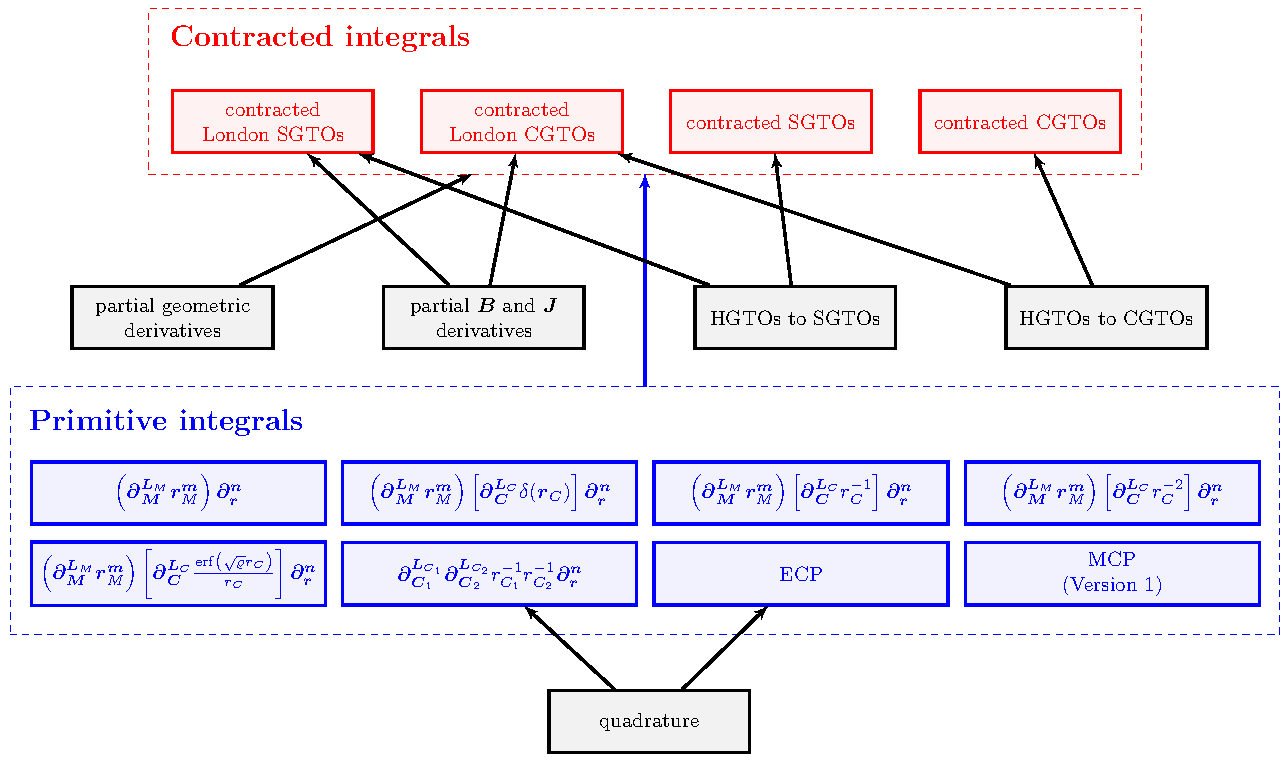
\includegraphics[width=15cm]{contrint.pdf}
  \caption{Illustration of the framework of \textsc{Gen1Int}.}
  \label{fig:framework}
\end{figure}

Last but not least, one of the most important part for a library is the test suite, we have prepared tests
(Fortran 90 and Python) for all the subroutines in \textsc{Gen1Int}. Please see Section~\ref{sect:test-suite}
for more details.

% data structure
\section{Data Structure in \textsc{Gen1Int}}
\label{sect:data-structure}

As aforementioned, we have divided \textsc{Gen1Int} into the following steps to get the contacted
integrals~(\ref{eq:oneint-init}). Before discussing the individual step in detail, we first consider one
of the most important left problem~---~the data structure in these steps. More explicitly, we need to
design the ordering of the returned contracted integrals, i.e., the angular parts (or $xyz$ powers),
sub-shells, the $xyz$ components of operators and different derivatives, which one is more
consecutive in memory? The factors affecting our choice are:
\begin{enumerate}
  \item complexity of the code by using the chosen data structure,
  \item efficiency of the code by the data structure and,
  \item complexity of further using the integrals by the data structure.
\end{enumerate}
As regards the third factor, it is apparent that we usually need to either contract these integrals with
density matrix, perform matrix operations with other integrals, or write them into file. Therefore,
the angular parts (or $xyz$ powers) and sub-shells should be the most consecutive ones. In \textsc{Gen1Int},
the final contracted integrals is hence always given in a five-dimensional array as
\begin{verbatim}
    contr_ints(num_gto_bra,num_contr_bra,num_gto_ket,num_contr_ket,num_opt)
\end{verbatim}
where the first and third dimensions are the angular parts (or $xyz$ powers) on bra and ket centers,
respectively. The second and fourth dimensions are respectively the sub-shells with the same
azimuthal quantum number (but different principal quantum numbers) on bra and ket centers.
The fifth dimension \verb|num_opt| represents all the $xyz$ components of different operators and
derivatives. In order to give a reasonable arrangement of these $xyz$ components, we consider
the steps of evaluating contracted integrals, where the ranks with underlines/overline are those
involved in current step\footnote{We would like to mention that there are usually nested loops
in the recurrence relations. It is said that it would be better make the number of iterations of outer
loop be fewer, whilst that of inner loop be more. This depends on the cache, pipelining and
predetermination of CPUs. However, the later two depend on specific CPUs. We therefore mainly
focus on increasing the CPU caching, i.e., we choose the data structure with more consecutive
data during each step.}:
\begin{enumerate}
  \item Recovering the total geometric derivatives
    \[
      \left\{\underbrace{\boldsymbol{l}_{\kappa},\text{contr}_{\text{bra}},%
      \boldsymbol{l}_{\lambda},\text{contr}_{\text{ket}},\boldsymbol{n},\boldsymbol{m},
      \boldsymbol{K}_{1},\boldsymbol{K}_{2},\boldsymbol{K}\mathrm{-}\boldsymbol{K}_{0},%
      \boldsymbol{L}_{1},\boldsymbol{L}_{2},\boldsymbol{L}\mathrm{-}\boldsymbol{L}_{0}}_{\text{consecutive}},%
      \overline{\boldsymbol{L}_{\kappa}},\overline{\boldsymbol{L}_{\lambda}},%
      \overline{\boldsymbol{L}_{\alpha}},\overline{\boldsymbol{L}_{\boldsymbol{M}}},%
      \overline{\boldsymbol{L}_{g}}\right\}
    \]
    from
    \[
      \left\{\underbrace{\boldsymbol{l}_{\kappa},\text{contr}_{\text{bra}},%
      \boldsymbol{l}_{\lambda},\text{contr}_{\text{ket}},\boldsymbol{n},\boldsymbol{m},
      \boldsymbol{K}_{1},\boldsymbol{K}_{2},\boldsymbol{K}\mathrm{-}\boldsymbol{K}_{0},%
      \boldsymbol{L}_{1},\boldsymbol{L}_{2},\boldsymbol{L}\mathrm{-}\boldsymbol{L}_{0}}_{\text{consecutive}},%
      \underline{\boldsymbol{L}_{\kappa}},\underline{\boldsymbol{L}_{\lambda}},%
      \underline{\boldsymbol{L}_{\alpha}},\underline{\boldsymbol{L}_{\boldsymbol{M}}}\right\};
    \]
%
  \item Recovering the geometric derivatives on dipole origin $\boldsymbol{r}_{M}$
    \[
      \left\{\underbrace{\boldsymbol{l}_{\kappa},\text{contr}_{\text{bra}},\boldsymbol{l}_{\lambda},%
      \text{contr}_{\text{ket}},\boldsymbol{n}}_{\text{consecutive}},\overline{\boldsymbol{m}},%
      \underbrace{\boldsymbol{K}_{1},\boldsymbol{K}_{2},\boldsymbol{K}\mathrm{-}\boldsymbol{K}_{0},%
      \boldsymbol{L}_{1},\boldsymbol{L}_{2},\boldsymbol{L}\mathrm{-}\boldsymbol{L}_{0},%
      \boldsymbol{L}_{\kappa},\boldsymbol{L}_{\lambda},\boldsymbol{L}_{\alpha}}_{\text{outer loop}},
      \overline{\boldsymbol{L}_{\boldsymbol{M}}}\right\}
    \]
    from
    \[
      \left\{\underbrace{\boldsymbol{l}_{\kappa},\text{contr}_{\text{bra}},\boldsymbol{l}_{\lambda},\text{contr}_{\text{ket}},%
      \boldsymbol{n}}_{\text{consecutive}},\underline{\boldsymbol{m}\mathrm{-}\boldsymbol{L}_{\boldsymbol{M}}},%
      \underbrace{\boldsymbol{K}_{1},\boldsymbol{K}_{2},\boldsymbol{K}\mathrm{-}\boldsymbol{K}_{0},%
      \boldsymbol{L}_{1},\boldsymbol{L}_{2},\boldsymbol{L}\mathrm{-}\boldsymbol{L}_{0},%
      \boldsymbol{L}_{\kappa},\boldsymbol{L}_{\lambda},\boldsymbol{L}_{\alpha}}_{\text{outer loop}}\right\};
    \]
%
  \item Recovering the total derivatives with respect to magnetic field and total rotational angular momentum by
    \begin{align}
      &\left\{\underbrace{\boldsymbol{l}_{\kappa},\text{contr}_{\text{bra}},%
      \boldsymbol{l}_{\lambda},\text{contr}_{\text{ket}},\boldsymbol{n},%
      \boldsymbol{m}\mathrm{-}\boldsymbol{L}_{\boldsymbol{M}}}_{\text{consecutive}},%
      \overline{\boldsymbol{K}_{1}},\overline{\boldsymbol{K}_{2}},%
      \overline{\boldsymbol{K}\mathrm{-}\boldsymbol{K}_{0}},%
      \overline{\boldsymbol{L}_{1}},\overline{\boldsymbol{L}_{2}},%
      \overline{\boldsymbol{L}\mathrm{-}\boldsymbol{L}_{0}},%
      \underbrace{\boldsymbol{L}_{\kappa},\boldsymbol{L}_{\lambda},%
      \boldsymbol{L}_{\alpha}}_{\text{outer loop}}\right\}\nonumber\\
      &\hspace{2em}=\sum_{\boldsymbol{K}'=\boldsymbol{0}}^{\boldsymbol{K}-\boldsymbol{K}_{0}}%
        \sum_{\boldsymbol{L}'=\boldsymbol{0}}^{\boldsymbol{L}-\boldsymbol{L}_{0}}%
        \binom{\boldsymbol{K}-\boldsymbol{K}_{0}}{\boldsymbol{K}'}%
        \binom{\boldsymbol{L}-\boldsymbol{L}_{0}}{\boldsymbol{L}'}\nonumber\\
      &\hspace{2em}\times\left\{\underbrace{\boldsymbol{l}_{\kappa},\text{contr}_{\text{bra}},%
      \boldsymbol{l}_{\lambda},\text{contr}_{\text{ket}},\boldsymbol{n},%
      \boldsymbol{m}\mathrm{-}\boldsymbol{L}_{\boldsymbol{M}}}_{\text{consecutive}},%
      \underline{\boldsymbol{K}_{1}\mathrm{+}\boldsymbol{K}'},%
      \underline{\boldsymbol{K}_{2}\mathrm{+}\boldsymbol{K}''},%
      \underline{\boldsymbol{L}_{1}\mathrm{+}\boldsymbol{L}'},%
      \underline{\boldsymbol{L}_{2}\mathrm{+}\boldsymbol{L}''},
      \underbrace{\boldsymbol{L}_{\kappa},\boldsymbol{L}_{\lambda},%
      \boldsymbol{L}_{\alpha}}_{\text{outer loop}}\right\};\nonumber
    \end{align}
%
  \item Recovering
    \[
      \left\{\underbrace{\boldsymbol{l}_{\kappa},\text{contr}_{\text{bra}},%
        \boldsymbol{l}_{\lambda},\text{contr}_{\text{ket}},\boldsymbol{n},%
        \boldsymbol{m}\mathrm{-}\boldsymbol{L}_{\boldsymbol{M}}}_{\text{consecutive}},%
        \overline{\boldsymbol{K}_{1}\mathrm{+}\boldsymbol{K}'},%
        \overline{\boldsymbol{K}_{2}\mathrm{+}\boldsymbol{K}''},%
        \overline{\boldsymbol{L}_{1}\mathrm{+}\boldsymbol{L}'},%
        \overline{\boldsymbol{L}_{2}\mathrm{+}\boldsymbol{L}''},%
        \overline{\boldsymbol{L}_{\kappa}},\overline{\boldsymbol{L}_{\lambda}},%
        \underbrace{\boldsymbol{L}_{\alpha}}_{\text{outer loop}}\right\}
    \]
    from
    \[
      \left\{\underbrace{\boldsymbol{l}_{\kappa},\text{contr}_{\text{bra}},%
        \boldsymbol{l}_{\lambda},\text{contr}_{\text{ket}},\boldsymbol{n},%
        \boldsymbol{m}\mathrm{-}\boldsymbol{L}_{\boldsymbol{M}}}_{\text{consecutive}},%
        \underline{\boldsymbol{N}_{1}},\underline{\boldsymbol{N}_{2}},%
        \underline{\boldsymbol{L}_{\kappa}},\underline{\boldsymbol{L}_{\lambda}},%
        \underbrace{\boldsymbol{L}_{\alpha}}_{\text{outer loop}}\right\};
      \]
%
  \item For contracted spherical Gaussians
    \begin{enumerate}
      \item Getting the contracted spherical Gaussian integrals from contracted Hermite Gaussian integrals by
        \[
          \sum_{|\boldsymbol{l}_{\kappa}|=l_{\kappa}}\sum_{|\boldsymbol{l}_{\lambda}|=l_{\lambda}}%
          S^{l_{\kappa}m_{\kappa}}_{\boldsymbol{l}_{\kappa}}S^{l_{\lambda}m_{\lambda}}_{\boldsymbol{l}_{\lambda}}%
          \sum_{ij}w_{i\kappa}w_{j\lambda}%
          \left\{\boldsymbol{l}_{\kappa},\boldsymbol{l}_{\lambda},\boldsymbol{n},%
          \boldsymbol{m}\mathrm{-}\boldsymbol{L}_{\boldsymbol{M}},%
          \boldsymbol{N}_{1},\boldsymbol{N}_{2},\boldsymbol{L}_{\kappa},%
          \boldsymbol{L}_{\lambda},\boldsymbol{L}_{\alpha},i,j\right\}_{\text{Herm}},
        \]
      \item Recovering primtive Hermite Gaussian integrals
        \[
          \left\{\overline{\boldsymbol{l}_{\kappa}},\overline{\boldsymbol{l}_{\lambda}},%
          \boldsymbol{n},\boldsymbol{m}\mathrm{-}\boldsymbol{L}_{\boldsymbol{M}},%
          \boldsymbol{N}_{1},\boldsymbol{N}_{2},%
          \overline{\boldsymbol{L}_{\kappa}},\overline{\boldsymbol{L}_{\lambda}},%
          \underbrace{\boldsymbol{L}_{\alpha},i,j}_{\text{outer loop}}\right\}_{\text{Herm}}
        \]
        from
        \[
          \left\{\overline{\boldsymbol{l}_{\kappa}\mathrm{+}\boldsymbol{L}_{\kappa}},%
          \overline{\boldsymbol{l}_{\lambda}\mathrm{+}\boldsymbol{L}_{\lambda}},%
          \boldsymbol{n},\boldsymbol{m}\mathrm{-}\boldsymbol{L}_{\boldsymbol{M}},%
          \boldsymbol{N}_{1},\boldsymbol{N}_{2},%
          \underbrace{\boldsymbol{L}_{\alpha},i,j}_{\text{outer loop}}\right\}_{\text{Herm}},
        \]
      \item Recovering
        \[
          \left\{\overline{\boldsymbol{l}_{\kappa}},\overline{\boldsymbol{l}_{\lambda}},%
          \boldsymbol{n},\boldsymbol{m}\mathrm{-}\boldsymbol{L}_{\boldsymbol{M}},%
          \overline{\boldsymbol{N}_{1}},\overline{\boldsymbol{N}_{2}},%
          \underbrace{\boldsymbol{L}_{\alpha},i,j}_{\text{outer loop}}\right\}_{\text{Herm}}
        \]
        from
        \[
          \left\{\underline{\boldsymbol{l}_{\kappa}},\underline{\boldsymbol{l}_{\lambda}},%
          \boldsymbol{n},\boldsymbol{m}\mathrm{-}\boldsymbol{L}_{\boldsymbol{M}},%
          \underbrace{\boldsymbol{L}_{\alpha},i,j}_{\text{outer loop}}\right\}_{\text{Herm}};
        \]
    \end{enumerate}
%
  \item For contracted Cartesian Gaussians
    \begin{enumerate}
      \item Recovering
        \[
          \left\{\overline{\boldsymbol{l}_{\kappa}},\text{contr}_{\text{bra}},%
          \overline{\boldsymbol{l}_{\lambda}},\text{contr}_{\text{ket}},%
          \boldsymbol{n},\boldsymbol{m}\mathrm{-}\boldsymbol{L}_{\boldsymbol{M}},%
          \overline{\boldsymbol{N}_{1}},\overline{\boldsymbol{N}_{2}},%
          \overline{\boldsymbol{L}_{\kappa}},\overline{\boldsymbol{L}_{\lambda}},%
          \underbrace{\boldsymbol{L}_{\alpha}}_{\text{outer loop}}\right\}
        \]
        from
        \begin{align}
          &\left\{\underline{\boldsymbol{l}_{\kappa}},\text{contr}_{\text{bra}},%
          \underline{\boldsymbol{l}_{\lambda}},\text{contr}_{\text{ket}},%
          \boldsymbol{n},\boldsymbol{m}\mathrm{-}\boldsymbol{L}_{\boldsymbol{M}},
          \underline{\boldsymbol{L}_{\kappa}},\underline{\boldsymbol{L}_{\lambda}},%
          \underbrace{\boldsymbol{L}_{\alpha}}_{\text{outer loop}}\right\}\nonumber\\
          &\hspace{2em}=\sum_{ij}w_{i\kappa}w_{j\lambda}%
          \left\{\boldsymbol{l}_{\kappa},\boldsymbol{l}_{\lambda},%
          \boldsymbol{n},\boldsymbol{m}\mathrm{-}\boldsymbol{L}_{\boldsymbol{M}},%
          \boldsymbol{L}_{\kappa},\boldsymbol{L}_{\lambda},\boldsymbol{L}_{\alpha},i,j\right\}_{\text{Cart}},\nonumber
        \end{align}
      \item Recovering primitive Cartesian Gaussian integrals
        \[
          \left\{\overline{\boldsymbol{l}_{\kappa}},\overline{\boldsymbol{l}_{\lambda}},%
          \boldsymbol{n},\boldsymbol{m}\mathrm{-}\boldsymbol{L}_{\boldsymbol{M}},
          \overline{\boldsymbol{L}_{\kappa}},\overline{\boldsymbol{L}_{\lambda}},%
          \underbrace{\boldsymbol{L}_{\alpha},i,j}_{\text{outer loop}}\right\}_{\text{Cart}}
        \]
        from primitive Hermite Gaussian integrals
        \[
          \left\{\underline{\boldsymbol{L}_{\kappa}},\underline{\boldsymbol{L}_{\lambda}},%
          \boldsymbol{n},\boldsymbol{m}\mathrm{-}\boldsymbol{L}_{\boldsymbol{M}},%
          \underbrace{\boldsymbol{L}_{\alpha},i,j}_{\text{outer loop}}\right\}_{\text{Herm}};
        \]
    \end{enumerate}
%
  \item Recovering different primitive Hermite Gausssin integrals %
    $\left\{\boldsymbol{l}_{\kappa},\boldsymbol{l}_{\lambda},\boldsymbol{n},%
      \boldsymbol{m}\mathrm{-}\boldsymbol{L}_{M},%
      \boldsymbol{L}_{\alpha},i,j\right\}_{\text{Herm}}$.
\end{enumerate}

Therefore, the fifth dimension is arranged in the order of
\begin{verbatim}
               num_elec, num_mom,
               num_mag_bra, num_mag_ket, num_mag_total,
               num_ram_bra, num_ram_ket, num_ram_total,
               num_geo_bra, num_geo_ket, num_geo_opt, num_geo_total,
\end{verbatim}
As regards the total geometric derivatives, the $xyz$ components of the first differentiated center
is the most consecutive part, followed by the second, third, ..., and the last differentiated center.

% geometric derivatives
\section{Geometric Derivatives}
\label{sect:geometric}

As mentioned previously, there are two tasks for geometric derivatives:
\begin{enumerate}
  \item Generating the total geometric derivatives
    $\prod^{N_{g}}\boldsymbol{\partial}_{\boldsymbol{R}_{g}}^{\boldsymbol{L}_{g}}$
    according to the given $N_{g}$ and number of atoms, avoiding
    repetition and omission, and arranging these geometric derivatives in a required sequence;
  \item Transferring the above generated total geometric derivatives to partial geometric derivatives
    on centers bra, ket, and/or centers in operator $\hat{O}_{\ell_{\beta}}^{\boldsymbol{K}_{0}\boldsymbol{L}_{0}}$.
\end{enumerate}

These questions will be addressed in the following two sections.

\subsection{Sequence of Total Geometric Derivatives}
\label{subsec:geom-total}

We first consider the question of generating all possible total geometric derivatives in a required
sequence. Let us consider the $g$-center $L$-th order total geometric derivatives (of an $N$-atom system)
\begin{equation}
  \label{eq:total-geom-derivatives}
  \boldsymbol{\partial}_{\boldsymbol{R}_{1}}^{\boldsymbol{L}_{1}}%
  \boldsymbol{\partial}_{\boldsymbol{R}_{2}}^{\boldsymbol{L}_{2}}\cdots%
  \boldsymbol{\partial}_{\boldsymbol{R}_{g}}^{\boldsymbol{L}_{g}}%
  \int\omega_{\kappa}^\ast(\boldsymbol{r};\boldsymbol{B},\boldsymbol{J})
  \hat{O}_{\ell_{\beta}}\left(\left\{\boldsymbol{r}_{C_{\alpha}}\right\},%
    \boldsymbol{\partial_{r}^{n}};\boldsymbol{B},\boldsymbol{J}\right)%
  \omega_{\lambda}(\boldsymbol{r};\boldsymbol{B},\boldsymbol{J})\mathrm{d}\boldsymbol{r},
\end{equation}
where
\begin{equation}
  \begin{cases}
    |\boldsymbol{L}_{g'}|\ge1,&(1\le g'\le g),\\
    \sum_{g'=1}^{g}|\boldsymbol{L}_{g'}|=L.
  \end{cases}
\end{equation}

The sequence of the total geometric derivatives represents by the sequence of the indices
(denoted as $\overline{R_{g'}}$, $1\le g'\le g$) of centers. We use an ascending order of the
indices in \textsc{Gen1Int}
\begin{equation}
  \label{eq:ascending-centers}
  1\le\overline{R_{1}}\le\overline{R_{2}}\le\dots\overline{R_{g}}\le N.
\end{equation}

In Ref.~\cite{bgkr}, we have developed a procedure to generate all the possible total geometric
derivatives by using the conception ``full arithmetic $N$-ary tree''. Taking fourth order total geometric
derivatives as an example, as shown in Fig. \ref{fig:n-ary-tree}, the task of finding required total
geometric derivatives could be done by the following steps:
\begin{enumerate}
  \item For a given path $\{\overline{R_{1}},\dots,\overline{R_{v-1}},\overline{R_{v}},%
    \overline{R_{v+1}},\dots,\overline{R_{L}}\}$ and ``height'' $v$\footnote{The height should be $v-1$.},
    we replace $\overline{R_{v}}$ with its sibling $\overline{R_{v}}+1$. Here $\overline{R_{v}}$
    should be the highest node which could be replaced, i.e., $\overline{R_{v+1}}=\dots=\overline{R_{L}}=N$.
  \item We then set $\overline{R_{v+1}}=\dots=\overline{R_{L}}=\overline{R_{v}}+1$. If the number of
    different centers in path\linebreak $\{\overline{R_{1}},\dots,\overline{R_{v-1}},\overline{R_{v}}+1, %
    \dots,\overline{R_{v}}+1\}$ is less than or equal to $N_{\alpha}+2$\footnote{$N_{\alpha}$
    is the number of centers in operator $\hat{O}_{\ell_{\beta}}^{\boldsymbol{K}_{0}\boldsymbol{L}_{0}}$.},
    we then choose this path\footnote{Differentiated centers are in the reverse order of this path.}
    and set $v=L$ ($\overline{R_{v}}+1<N$) or $v=v-1$ ($\overline{R_{v}}+1=N$);
    otherwise, we set $v=v-1$ and back to previous step to generate satisfied path.
\end{enumerate}
This procedure could start from the leftmost path $\{\underbrace{11\dots1}_{L}\}$ and $v=L$, and
end at the path $\{\underbrace{NN\dots N}_{L}\}$. All required total geometric derivatives could be
generated, without repetition and omission.
\begin{figure}[hbtp]
  \centering
  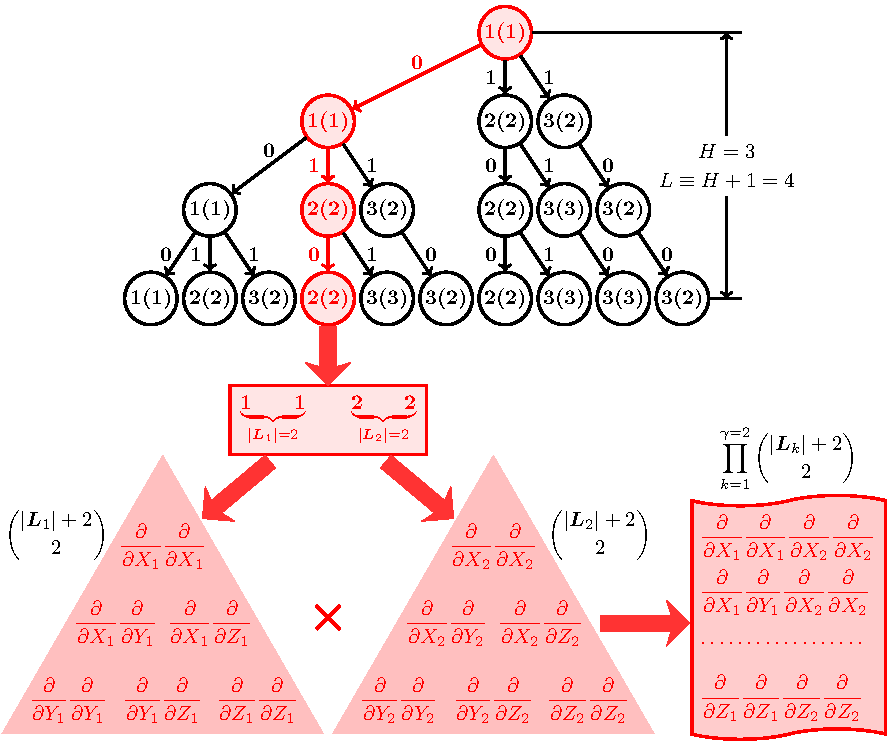
\includegraphics[width=12cm]{n_ary_tree.pdf}
  \caption{A typical ``full arithmetic $3$-ary tree'' with height $H=3$ started from the first atom. The numbers
  in the parentheses, and along with the arrows (paths between two nodes) are the weights of the corresponding
  node and path. The selected path from the ``root'' to the ``leaf'' node (denoted as red color) represents the
  generated differentiated geometric centers, while the red triangles and flag are the generated two center
  fourth order total geometric derivatives.}
  \label{fig:n-ary-tree}
\end{figure}

This procedure has been implemented in file \verb|geom_total.F90| with the subroutines detailed
in Table~\ref{tab:geom-total}, where ``\textbf{Public}'' subroutines could be called by users in their
own codes, and ``\textbf{Private}'' subroutines are usually not be called by the users.
\begin{center}
  \begin{longtable}{l|p{1.1cm}|p{2.3cm}p{7.6cm}}
    \caption{Subroutines of total geometric derivatives in \textsc{Gen1Int}.}
    \label{tab:geom-total}\\
    \hline\hline
    \endfirsthead
%
    \multicolumn{4}{c}{{\bfseries\tablename~\thetable{} -- continued from previous page}}\\
    \hline\hline
    \endhead
%
    \hline
    \multicolumn{4}{r}{{Continued on next page}}\\
    \hline
    \endfoot
%
    \hline\hline
    \endlastfoot
%
    \multicolumn{4}{l}{\textbf{Public}}\\
    \hline
    \verb|geom_total_tree_init|\index{\textsl{public} \texttt{geom\_total\_tree\_init}} & %
      \multicolumn{3}{p{11cm}}{Returns the total number of different paths, and generates the first path.}\\
    \cline{2-4}
    & \textbf{In} & \verb|num_atoms| & number of atoms ($N$)\\
    \cline{3-4}
    & & \verb|order_geo| & order of total geometric derivatives ($L$)\\
    \cline{3-4}
    & & \verb|max_num_cent| & maximum number of differentiated centers ($g$)\\
    \cline{2-4}
    & \textbf{Out} & \verb|num_paths| & total number of different paths\\
    \cline{3-4}
    & & \verb|visit_height| & ``height'' of atom to visit ($v$)\\
    \cline{3-4}
    & & \verb|idx_node| & indices of the selected atom nodes ($\{\overline{R_{1}},\overline{R_{2}},\dots,\overline{R_{L}}\}$)\\
    \cline{3-4}
    & & \verb|wt_node| & weights of the selected atom nodes\\
    \cline{3-4}
    & & \verb|idx_cent| & indices of generated differentiated centers\\
    \cline{3-4}
    & & \verb|order_cent| & order of derivatives of the differentiated centers\\
    \cline{3-4}
    & & \verb|num_geo_cent| & number of all geometric derivatives for this generated path %
      ($\prod_{g'=1}^{g}\binom{|\boldsymbol{L}_{g'}|+2}{2}$)\\
    \hline
    \verb|geom_total_tree_search|\index{\textsl{public} \texttt{geom\_total\_tree\_search}} & %
      \multicolumn{3}{p{11cm}}{Searches for the next satisfied path from a given path, could be called recursively.}\\
%
    \cline{2-4}
    & \textbf{In} & \verb|num_atoms| & number of atoms ($N$)\\
    \cline{3-4}
    & & \verb|order_geo| & order of total geometric derivatives ($L$)\\
    \cline{3-4}
    & & \verb|max_num_cent| & maximum number of differentiated centers ($g$)\\
    \cline{2-4}
    & \textbf{InOut} & \verb|visit_height| & ``height'' of atom to visit ($v$)\\
    \cline{3-4}
    & & \verb|idx_node| & indices of the selected atom nodes ($\{\overline{R_{1}},\overline{R_{2}},\dots,\overline{R_{L}}\}$)\\
    \cline{3-4}
    & & \verb|wt_node| & weights of the selected atom nodes\\
    \cline{3-4}
    & & \verb|idx_cent| & indices of generated differentiated centers\\
    \cline{3-4}
    & & \verb|order_cent| & order of derivatives of the differentiated centers\\
    \cline{2-4}
    & \textbf{Out} & \verb|num_geo_cent| & number of all geometric derivatives for this generated path %
      ($\prod_{g'=1}^{g}\binom{|\boldsymbol{L}_{g'}|+2}{2}$)\\
    \hline
    \multicolumn{4}{l}{\textbf{Private}}\\
    \hline
    \verb|geom_total_num_paths|\index{\textsl{private} \texttt{geom\_total\_num\_paths}} & %
      \multicolumn{3}{p{11cm}}{Computes the total number of different paths.}\\
    \cline{2-4}
    & \textbf{In} & \verb|num_atoms| & number of atoms ($N$)\\
    \cline{3-4}
    & & \verb|order_geo| & order of total geometric derivatives ($L$)\\
    \cline{3-4}
    & & \verb|max_num_cent| & maximum number of differentiated centers ($g$)\\
    \cline{2-4}
    & \textbf{Out} & \verb|num_paths| & total number of different paths %
      ($\sum_{g'=1}^{\min(N_{g},L)}\binom{N}{g'}\binom{L-1}{g'-1}$)\\
    \hline
    \verb|geom_total_new_path|\index{\textsl{private} \texttt{geom\_total\_new\_path}} & %
      \multicolumn{3}{p{11cm}}{Generates a new path of differentiated centers from a given path, %
        the first path will return for giving the last path.}\\
    \cline{2-4}
    & \textbf{In} & \verb|num_atoms| & number of atoms ($N$)\\
    \cline{3-4}
    & & \verb|order_geo| & order of total geometric derivatives ($L$)\\
    \cline{2-4}
    & \textbf{InOut} & \verb|visit_height| & ``height'' of atom to visit ($v$)\\
    \cline{3-4}
    & & \verb|idx_node| & indices of the selected atom nodes ($\{\overline{R_{1}},\overline{R_{2}},\dots,\overline{R_{L}}\}$)\\
    \cline{3-4}
    & & \verb|wt_node| & weights of the selected atom nodes\\
  \end{longtable}
\end{center}

Last but not least, the number of redundant total geometric derivatives for a given path
in Fig.~\ref{fig:n-ary-tree} could be calculated as
\begin{equation}
  3^{L}\prod_{g'=1}^{g}\binom{L-\sum_{n=1}^{g'-1}|\boldsymbol{L}_{n}|}{|\boldsymbol{L}_{g'}|},
\end{equation}
as implemented in subroutine \verb|geom_total_num_redunt|\index{\textsl{private} \texttt{geom\_total\_num\_redunt}}.

\subsection{Partial Geometric Derivatives}
\label{subsec:geom-part}

After generating the differentiated centers
$\left\{\boldsymbol{R}_{1},\boldsymbol{R}_{2},\cdots,\boldsymbol{R}_{g}\right\}$
and their orders of total geometric derivatives
$\left\{|\boldsymbol{L}_{1}|,|\boldsymbol{L}_{2}|,\cdots,|\boldsymbol{L}_{g}|\right\}$,
the left problems are
\begin{enumerate}
  \item transferring the generated total geometric derivatives to partial geometric derivatives
on centers of bra, ket and/or operator $\hat{O}_{\ell_{\beta}}^{\boldsymbol{K}_{0}\boldsymbol{L}_{0}}$;
  \item after calculations, retrieving the total geometric derivatives from these partial geometric derivatives.
\end{enumerate}

Suppose the centers of bra, ket and/or operator $\hat{O}_{\ell_{\beta}}^{\boldsymbol{K}_{0}\boldsymbol{L}_{0}}$
are $\left\{\boldsymbol{R}_{\kappa},\boldsymbol{R}_{\lambda},\boldsymbol{R}_{\alpha},\cdots\right\}$. In the first
step, we could compare the indices of these centers with those of differentiated centers
$\left\{\boldsymbol{R}_{1},\boldsymbol{R}_{2},\cdots,\boldsymbol{R}_{g}\right\}$ when $g\le N_{\alpha}+2$.
If there are identical centers in those of bra, ket and/or operator $\hat{O}_{\ell_{\beta}}^{\boldsymbol{K}_{0}\boldsymbol{L}_{0}}$,
let us say there are $N_{\beta}$ identical centers
$\left\{\boldsymbol{R}_{\beta_{1}},\boldsymbol{R}_{\beta_{2}},\cdots,\boldsymbol{R}_{\beta_{N_{\beta}}}\right\}$,
which are also identical with the differentiated center $\boldsymbol{R}_{\beta}$ in the total geometric derivatives,
and order $|\boldsymbol{L}_{\beta}|$. We then have, according to the multinomial theorem
(\url{http://en.wikipedia.org/wiki/Multinomial_theorem}), the following partial geometric derivatives
\begin{equation}
  \sum_{\sum_{k=1}^{N_{\beta}}|\boldsymbol{l}_{k}|=|\boldsymbol{L}_{\beta}|}%
    \binom{|\boldsymbol{L}_{\beta}|}{|\boldsymbol{l}_{1}|,|\boldsymbol{l}_{2}|,\cdots,|\boldsymbol{l}_{N_{\beta}}|}%
    \prod_{k=1}^{N_{\beta}}\boldsymbol{\partial}_{\boldsymbol{R}_{\beta_{k}}}^{\boldsymbol{l}_{k}},
\end{equation}
where
\begin{align}
  \binom{|\boldsymbol{L}_{\beta}|}{|\boldsymbol{l}_{1}|,|\boldsymbol{l}_{2}|,\cdots,|\boldsymbol{l}_{N_{\beta}}|}
  &=\frac{|\boldsymbol{L}_{\beta}|!}{|\boldsymbol{l}_{1}|!|\boldsymbol{l}_{2}|!\cdots|\boldsymbol{l}_{N_{\beta}}|!}\\
  &=\binom{|\boldsymbol{l}_{1}|}{|\boldsymbol{l}_{1}|}\binom{|\boldsymbol{l}_{1}|+|\boldsymbol{l}_{2}|}{|\boldsymbol{l}_{2}|}%
    \cdots\binom{|\boldsymbol{l}_{1}|+|\boldsymbol{l}_{2}|+\cdots+|\boldsymbol{l}_{N_{\beta}}|}{|\boldsymbol{l}_{N_{\beta}}|}\\
  &=\prod_{k=1}^{N_{\beta}}\binom{\sum_{k'=1}^{k}|\boldsymbol{l}_{k'}|}{|\boldsymbol{l}_{k}|},
\end{align}
is the multinomial coefficient. The sum of all multinomial coefficients is
\begin{equation}
  \sum_{\sum_{k=1}^{N_{\beta}}|\boldsymbol{l}_{k}|=|\boldsymbol{L}_{\beta}|}%
    \binom{|\boldsymbol{L}_{\beta}|}{|\boldsymbol{l}_{1}|,|\boldsymbol{l}_{2}|,\cdots,|\boldsymbol{l}_{N_{\beta}}|}%
  =N_{\beta}^{|\boldsymbol{L}_{\beta}|},
\end{equation}
and the number of multinomial coefficients (or the number of terms in multinomial sum)
$\#_{|\boldsymbol{L}_{\beta}|,N_{\beta}}$ is
\begin{equation}
  \#_{|\boldsymbol{L}_{\beta}|,N_{\beta}}
  =\binom{|\boldsymbol{L}_{\beta}|+N_{\beta}-1}{N_{\beta}-1}
  =\binom{|\boldsymbol{L}_{\beta}|+N_{\beta}-1}{|\boldsymbol{L}_{\beta}|}.
\end{equation}

As pointed out in our recent work~\cite{bgkr}, sometimes this expansion is however not efficient,
further simplifications could be made by using the translational invariance~\cite{Komornicki:CPL45:595,Kahn:JCP75:3962}.
In Ref.~\cite{bgkr}, we have given the possible partial geometric derivatives for operators with the
number of centers $N_{\alpha}\le2$ and in the case of $\overline{R_{\kappa}}=\overline{R_{\lambda}}$.
These results are also shown here in Table~\ref{tab:geometric-derivatives-op012}.
\begin{table}[hbtp]
  \centering
  \caption{Possible partial geometric derivatives for $\overline{R_{\kappa}}=\overline{R_{\lambda}}$ and
  the operator with the number of centers $N_{\alpha}\le2$.}
  \label{tab:geometric-derivatives-op012}
  \begin{tabular}{c|c|c}
    \hline\hline
    & Identical centers & Possible partial geometric derivatives\\
    \hline
    $N_{\alpha}=0$ & $\overline{R_{\kappa}}=\overline{R_{\lambda}}$ & $0$\\
    \hline
    $N_{\alpha}=1$ & $\overline{R_{\kappa}}=\overline{R_{\lambda}}=\overline{C_{1}}$ & $0$\\
                              & $\overline{R_{\kappa}}=\overline{R_{\lambda}}\ne\overline{C_{1}}$ &%
                                 $(-1)^{|\boldsymbol{L}_{\kappa}|}%
                                   \boldsymbol{\partial}_{\boldsymbol{C}_{1}}^{\boldsymbol{L}_{C_{1}}+\boldsymbol{L}_{\kappa}}$\\
    \hline
    $N_{\alpha}=2$ & $\overline{R_{\kappa}}=\overline{R_{\lambda}}=\overline{C_{1}}=\overline{C_{2}}$ & $0$\\
                              & $\overline{R_{\kappa}}=\overline{R_{\lambda}}=\overline{C_{1}}\ne\overline{C_{2}}$ &%
                                 $(-1)^{|\boldsymbol{L}_{\kappa}|}%
                                   \boldsymbol{\partial}_{\boldsymbol{C}_{2}}^{\boldsymbol{L}_{C_{2}}+\boldsymbol{L}_{\kappa}}$\\
                              & $(\overline{R_{\kappa}}=\overline{R_{\lambda}})\ne(\overline{C_{1}}=\overline{C_{2}})$ &%
                                 $(-1)^{|\boldsymbol{L}_{\kappa}|}%
                                   \sum_{\boldsymbol{l}_{1}=\boldsymbol{0}}^{\boldsymbol{L}_{\kappa}+\boldsymbol{L}_{C_{1}}}%
                                   \binom{\boldsymbol{L}_{\kappa}+\boldsymbol{L}_{C_{1}}}{\boldsymbol{l}_{1}}%
                                   \boldsymbol{\partial}_{\boldsymbol{C}_{1}}^{\boldsymbol{l}_{1}}%
                                   \boldsymbol{\partial}_{\boldsymbol{C}_{2}}^{\boldsymbol{L}_{\kappa}%
                                     +\boldsymbol{L}_{C_{1}}-\boldsymbol{l}_{1}}$\\
                              & $\overline{R_{\kappa}}=\overline{R_{\lambda}}\ne\overline{C_{1}}\ne\overline{C_{2}}$ &%
                                 $\sum_{\boldsymbol{l}_{\kappa}=\boldsymbol{0}}^{\boldsymbol{L}_{\kappa}}%
                                   \binom{\boldsymbol{L}_{\kappa}}{\boldsymbol{l}_{\kappa}}%
                                   \boldsymbol{\partial}_{\boldsymbol{R}_{\kappa}}^{\boldsymbol{l}_{\kappa}}%
                                   \boldsymbol{\partial}_{\boldsymbol{R}_{\lambda}}^{\boldsymbol{L}_{\kappa}-\boldsymbol{l}_{\kappa}}%
                                   \boldsymbol{\partial}_{\boldsymbol{C}_{1}}^{\boldsymbol{L}_{C_{1}}}%
                                   \boldsymbol{\partial}_{\boldsymbol{C}_{2}}^{\boldsymbol{L}_{C_{2}}}$\\
    \hline\hline
  \end{tabular}
\end{table}

Being aware of that most operators in one-electron integrals have two centers at maximum, we
therefore only consider the operators with $N_{\alpha}\le2$ centers in current version of
\textsc{Gen1Int} by hand coding implementation of Table~\ref{tab:geometric-derivatives-op012}.
The subroutines related to partial geometric derivatives are implemented in files \verb|geom_part_zero.F90|,
\verb|geom_part_one.F90| and \verb|geom_part_two.F90|.

\fixme{Describe} \verb|shell_scatter.F90| and \verb|shell_gather.F90| ...
\fixme{The procedure of scattering shells} is given in Fig.~\ref{fig:shell-scatter},
and implemented in file \verb|shell_scatter.F90| ...
\begin{figure}[hbtp]
  \centering
  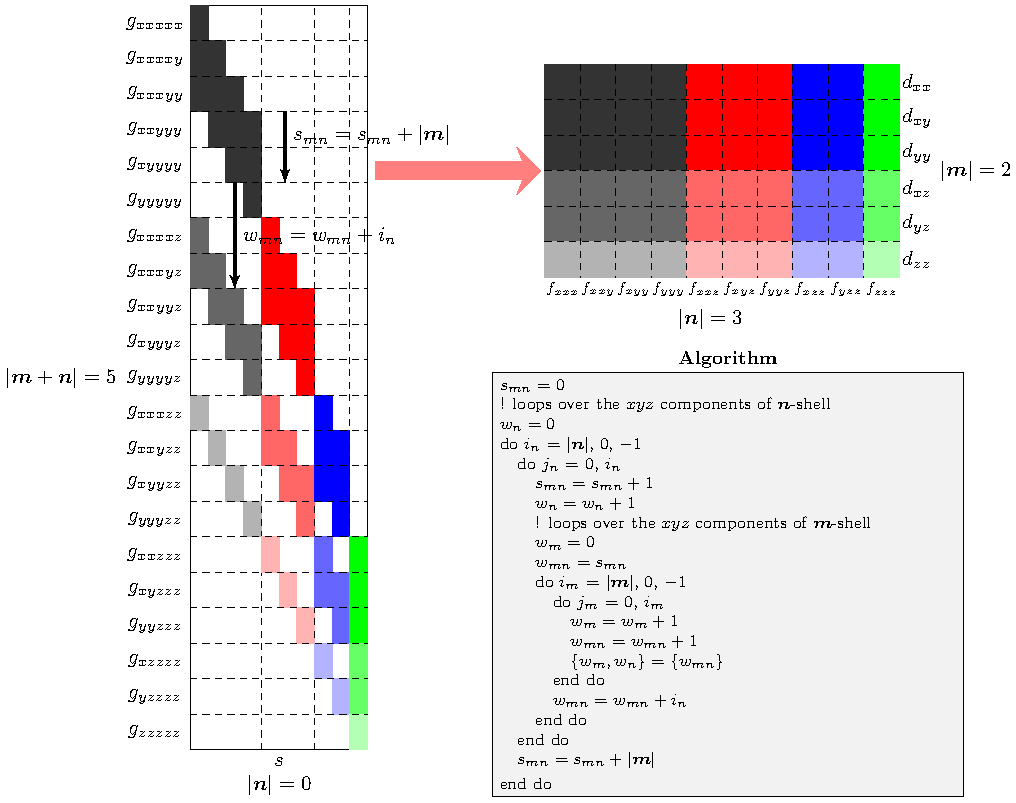
\includegraphics[width=6.5in]{shell_scatter.pdf}
  \caption{Procedure of scattering shells.}
  \label{fig:shell-scatter}
\end{figure}

\fixme{\begin{equation}
  |\boldsymbol{m}|+|\boldsymbol{n}|+1 %
    <(|\boldsymbol{n}|+1)\frac{(|\boldsymbol{m}|+1)(|\boldsymbol{m}|+2)}{2}
\end{equation}}

% magnetic and total rotational angular momentum derivatives
\section{Magnetic and Total Rotational Angular Momentum Derivatives}
\label{sect:magnetic}

\fixme{We assume that} $\boldsymbol{K}_{0}$ and $\boldsymbol{L}_{0}$ in the operator
$\hat{O}_{\ell_{\beta}}^{\boldsymbol{K}_{0}\boldsymbol{L}_{0}}$ could run all the
$xyz$ components in the triangle ...

In order to evaluate
\begin{equation}
  \boldsymbol{\partial}_{\boldsymbol{R}_{\kappa}}^{\boldsymbol{L}_{\kappa}}%
  \boldsymbol{\partial}_{\boldsymbol{R}_{\lambda}}^{\boldsymbol{L}_{\lambda}}%
  \int\left[\boldsymbol{\partial}_{\boldsymbol{B}}^{\boldsymbol{K}_{1}}%
      \omega_{\kappa}^{*}(\boldsymbol{r};\boldsymbol{B})\right]_{\boldsymbol{B}=\boldsymbol{0}}%
    \hat{O}\left(\left\{\boldsymbol{r}_{C_{\alpha}}\right\},\boldsymbol{\partial_{r}^{n}}\right)%
    \left[\boldsymbol{\partial}_{\boldsymbol{B}}^{\boldsymbol{K}_{2}}%
      \omega_{\lambda}(\boldsymbol{r};\boldsymbol{B})\right]_{\boldsymbol{B}=\boldsymbol{0}}\mathrm{d}\boldsymbol{r}
\end{equation}
to any order $\boldsymbol{K}_{1}$ and $\boldsymbol{K}_{2}$, we introduce the following auxiliary integral
\begin{equation}
  \boldsymbol{\partial}_{\boldsymbol{R}_{\kappa}}^{\boldsymbol{L}_{\kappa}}%
  \boldsymbol{\partial}_{\boldsymbol{R}_{\lambda}}^{\boldsymbol{L}_{\lambda}}%
  \int\boldsymbol{r}_{P}^{\boldsymbol{N}_{1}}%
    \left[\boldsymbol{\partial}_{\boldsymbol{B}}^{\boldsymbol{K}_{1}}%
      \omega_{\kappa}^{*}(\boldsymbol{r};\boldsymbol{B})\right]_{\boldsymbol{B}=\boldsymbol{0}}%
    \hat{O}\left(\left\{\boldsymbol{r}_{C_{\alpha}}\right\},\boldsymbol{\partial_{r}^{n}}\right)%
    \boldsymbol{r}_{P}^{\boldsymbol{N}_{2}}%
    \left[\boldsymbol{\partial}_{\boldsymbol{B}}^{\boldsymbol{K}_{2}}%
      \omega_{\lambda}(\boldsymbol{r};\boldsymbol{B})\right]_{\boldsymbol{B}=\boldsymbol{0}}\mathrm{d}\boldsymbol{r},
\end{equation}

\fixme{Describe} how to perform this recurrence relations and sum ....

\section{Contracted Integrals}
\label{sect:contr-ints}

\fixme{Describe} subroutine \verb|const_contr_ints| in file \verb|const_contr_ints.F90| which performs the
contractions~(\ref{eq:nonlao-aux-int-cart}) and (\ref{eq:nonlao-aux-int-herm}) ...

\fixme{Describe} all the subroutines related to contracted integrals ...

% implemented one-electron operators
\section{One-electron Operators in \textsc{Gen1Int}}
\label{sect:operators}

We first discuss the evaluation of basic integral $\left[\boldsymbol{l}_{\kappa}\boldsymbol{l}_{\lambda}\Big|%
\hat{O}_{\ell_{\beta}}^{\boldsymbol{K}_{0}\boldsymbol{L}_{0}}\right]_{ij}$ with the operator
$\hat{O}_{\ell_{\beta}}^{\boldsymbol{K}_{0}\boldsymbol{L}_{0}}$ being the form
$\hat{O}_{\ell_{\beta}}^{\boldsymbol{K}_{0}\boldsymbol{L}_{0}}%
\left(\left\{\boldsymbol{r}_{C_{\alpha}}\right\},\boldsymbol{\partial_{r}^{n}}\right)
=\bar{C}f\left(\left\{\boldsymbol{r}_{C_{\alpha}}\right\}\right)\boldsymbol{\partial}_{\boldsymbol{r}}^{\boldsymbol{n}}$.
The cases of effective core potential and model core potential (Version 1) could be
obtained in the similar way. By substituting the explicit form of the operator into the basic integral~(\ref{eq:basic-int}),
we get~\cite{Gao:IJQC:2010,bgkrth-a,bgkr}
\begin{align}
  \left[\boldsymbol{l}_{\kappa}\boldsymbol{l}_{\lambda}\Big|%
    \hat{O}_{\ell_{\beta}}^{\boldsymbol{K}_{0}\boldsymbol{L}_{0}}\right]_{ij}
  &=\bar{C}(-2b_{j\lambda})^{|\boldsymbol{n}|}%
    \frac{\boldsymbol{\partial}_{\boldsymbol{R}_{\kappa}}^{\boldsymbol{l}_{\kappa}}}%
      {(2a_{i\kappa})^{|\boldsymbol{l}_{\kappa}|}}%
    \frac{\boldsymbol{\partial}_{\boldsymbol{R}_{\lambda}}^{\boldsymbol{l}_{\lambda}\mathrm{+}\boldsymbol{n}}}%
      {(2b_{j\lambda})^{|\boldsymbol{l}_{\lambda}|\mathrm{+}|\boldsymbol{n}|}}%
    \left[\mathrm{e}^{-u_{ij}R_{\kappa\lambda}^2}\int%
      f\left(\left\{\boldsymbol{r}_{C_{\alpha}}\right\}\right)%
        \mathrm{e}^{-p_{ij}r_{\gamma}^2}\mathrm{d}\boldsymbol{r}\right]\\
  &\equiv\bar{C}(-2b_{j\lambda})^{|\boldsymbol{n}|}%
    \left[\boldsymbol{l}_{\kappa},\boldsymbol{l}_{\lambda}\mathrm{+}\boldsymbol{n}%
      \Big|f\left(\left\{\boldsymbol{r}_{C_{\alpha}}\right\}\right)\right]_{ij},\nonumber
\end{align}
where we have introduced the quantities 
\begin{align}
  \label{eq:prule}
  p_{ij}=a_{i\kappa}+b_{j\lambda}, \quad
  u_{ij}=\frac{a_{i\kappa}b_{j\lambda}}{p_{ij}}, \quad
  \boldsymbol{R}_{\gamma}=\frac{a_{i\kappa}\boldsymbol{R}_{\kappa}+b_{j\lambda}\boldsymbol{R}_{\lambda}}{p_{ij}}.
\end{align}

The recurrence relations of $\bar{C}(-2b_{j\lambda})^{|\boldsymbol{n}|}%
\left[\boldsymbol{l}_{\kappa},\boldsymbol{l}_{\lambda}\mathrm{+}\boldsymbol{n}%
\Big|f\left(\left\{\boldsymbol{r}_{C_{\alpha}}\right\}\right)\right]_{ij}$ for different $f\left(\left\{\boldsymbol{r}_{C_{\alpha}}\right\}\right)$
have been discussed in Ref.~\cite{Gao:IJQC:2010,bgkrth-a,bgkr}. We will, in the following sections, discuss
the implementation of these recurrence relations.

% electronic derivatives
\subsection{Electronic Derivatives}
\label{subsec:elec-deriv}

The electronic derivatives could be recovered through
\begin{equation}
  \bar{C}\left[\boldsymbol{l}_{\kappa}\boldsymbol{l}_{\lambda}\Big|%
    f\left(\left\{\boldsymbol{r}_{C_{\alpha}}\right\}\right)%
    \boldsymbol{\partial}_{\boldsymbol{r}}^{\boldsymbol{n}}\right]_{ij}
  \equiv\bar{C}(-2b_{j\lambda})^{|\boldsymbol{n}|}%
    \left[\boldsymbol{l}_{\kappa},\boldsymbol{l}_{\lambda}\mathrm{+}\boldsymbol{n}%
      \Big|f\left(\left\{\boldsymbol{r}_{C_{\alpha}}\right\}\right)\right]_{ij},
\end{equation}
or in a more compact form
\begin{equation}
  \left\{\boldsymbol{l}_{\lambda},\boldsymbol{n}\right\}
    =\left\{\boldsymbol{l}_{\lambda}\mathrm{+}\boldsymbol{n}\right\}.
\end{equation}

\fixme{The electronic derivatives could be recovered by} calling the subroutine \verb|shell_scatter|
(see Section~\ref{subsec:geom-part}) ...

% Cartesian multipole moments
\subsection{Cartesian Multipole Moments}
\label{subsec:carmom}

The operator of Cartesian multipole moments can be written as follows
\begin{equation}
  \hat{O}_{\ell_{\beta}}^{\boldsymbol{K}_{0}\boldsymbol{L}_{0}}%
    =\bar{C}\left(\boldsymbol{\partial}_{\boldsymbol{M}}^{\boldsymbol{L}_{M}}\boldsymbol{r}_{M}^{\boldsymbol{m}}\right)%
      \boldsymbol{\partial}_{\boldsymbol{r}}^{\boldsymbol{n}}.
\end{equation}

The electronic derivatives have been discussed in previous section~\ref{subsec:elec-deriv}.
We will, in current section, discuss in detail about the evaluation of the integrals of the operator
$\bar{C}(-2b_{j\lambda})^{|\boldsymbol{n}|}%
\left(\boldsymbol{\partial}_{\boldsymbol{M}}^{\boldsymbol{L}_{M}}\boldsymbol{r}_{M}^{\boldsymbol{m}}\right)$.

\fixme{By gluing the subroutines together}, we get the subroutine \verb|prim_hgto_carmom|
which returns the Cartesian multipole moment integrals of given primitive Hermite Gaussians on bra
and ket centers. Describe \verb|prim_hgto_carmom| in detail ...

\subsubsection{Geometric Derivatives of Dipole Origin}

The geometric derivatives of dipole origin $\boldsymbol{r}_{M}$ can be further written as
\begin{equation}
  \boldsymbol{\partial}_{\boldsymbol{M}}^{\boldsymbol{L}_{M}}\boldsymbol{r}_{M}^{\boldsymbol{m}} %
    =\frac{(-1)^{|\boldsymbol{L}_{M}|}\boldsymbol{m}!}{(\boldsymbol{m}-\boldsymbol{L}_{M})!} %
      \boldsymbol{r}_{M}^{\boldsymbol{m}-\boldsymbol{L}_{M}},
\end{equation}
where we have required that
\begin{equation}
  \boldsymbol{m}\ge\boldsymbol{L}_{M}.
\end{equation}

Therefore, the integrals of geometric derivatives of dipole origin
$\boldsymbol{\partial}_{\boldsymbol{M}}^{\boldsymbol{L}_{M}}\boldsymbol{r}_{M}^{\boldsymbol{m}}$
in a multi-dimensional array $\left\{1\mathrm{:}N_{\boldsymbol{L}_{M}},1\mathrm{:}N_{\boldsymbol{m}}\right\}$,
could be retrieved from the integrals of lower order Cartesian multipole moments
$\boldsymbol{r}_{M}^{\boldsymbol{m}-\boldsymbol{L}_{M}}$ in an array
$\left\{1\mathrm{:}N_{\boldsymbol{m}-\boldsymbol{L}_{M}}\right\}$, where
\begin{align}
  N_{\boldsymbol{L}_{M}}%
    &=\frac{(|\boldsymbol{L}_{M}|+1)(|\boldsymbol{L}_{M}|+2)}{2},\\
  N_{\boldsymbol{m}}%
    &=\frac{(|\boldsymbol{m}|+1)(|\boldsymbol{m}|+2)}{2},\\
  N_{\boldsymbol{m}-\boldsymbol{L}_{M}}%
    &=\frac{(|\boldsymbol{m}|-|\boldsymbol{L}_{M}|+1)(|\boldsymbol{m}|-|\boldsymbol{L}_{M}|+2)}{2},
\end{align}
as illustrated in Table~\ref{tab:geom-diporg}. The procedure of retrieving the integrals of geometric
derivatives of dipole origin $\boldsymbol{\partial}_{\boldsymbol{M}}^{\boldsymbol{L}_{M}}\boldsymbol{r}_{M}^{\boldsymbol{m}}$
has been implemented in file \verb|carmom_deriv.F90|.
\begin{table}[hbtp]
  \centering
  \caption{Retrieving integrals of $\boldsymbol{\partial}_{\boldsymbol{M}}^{\boldsymbol{3}}\boldsymbol{r}_{M}^{\boldsymbol{5}}$
    through those of $\boldsymbol{r}_{M}^{\boldsymbol{2}}$.}
  \label{tab:geom-diporg}
  \begin{tabular}{c||c|c|c|c||c|c|c||c|c||c}
    \hline
    & $\partial_{xxx}$ & $\partial_{xxy}$ & $\partial_{xyy}$ & $\partial_{yyy}$ & $\partial_{xxz}$ %
      & $\partial_{xyz}$ & $\partial_{yyz}$ & $\partial_{xzz}$ & $\partial_{yzz}$ & $\partial_{zzz}$\\
    \hline
    $r_{xxxxx}$ & $r_{xx}$ & 0 & 0 & 0 & 0 & 0 & 0 & 0 & 0 & 0\\
    \hline
    $r_{xxxxy}$ & $r_{xy}$ & $r_{xx}$ & 0 & 0 & 0 & 0 & 0 & 0 & 0 & 0\\
    \hline
    $r_{xxxyy}$ & $r_{yy}$ & $r_{xy}$ & $r_{xx}$ & 0 & 0 & 0 & 0 & 0 & 0 & 0\\
    \hline
    $r_{xxyyy}$ & 0 & $r_{yy}$ & $r_{xy}$ & $r_{xx}$ & 0 & 0 & 0 & 0 & 0 & 0\\
    \hline
    $r_{xyyyy}$ & 0 & 0 & $r_{yy}$ & $r_{xy}$ & 0 & 0 & 0 & 0 & 0 & 0\\
    \hline
    $r_{yyyyy}$ & 0 & 0 & 0 & $r_{yy}$ & 0 & 0 & 0 & 0 & 0 & 0\\
    \hline\hline
    $r_{xxxxz}$ & $r_{xz}$ & 0 & 0 & 0 & $r_{xx}$ & 0 & 0 & 0 & 0 & 0\\
    \hline
    $r_{xxxyz}$ & $r_{yz}$ & $r_{xz}$ & 0 & 0 & $r_{xy}$ & $r_{xx}$ & 0 & 0 & 0 & 0\\
    \hline
    $r_{xxyyz}$ & 0 & $r_{yz}$ & $r_{xz}$ & 0 & $r_{yy}$ & $r_{xy}$ & $r_{xx}$ & 0 & 0 & 0\\
    \hline
    $r_{xyyyz}$ & 0 & 0 & $r_{yz}$ & $r_{xz}$ & 0 & $r_{yy}$ & $r_{xy}$ & 0 & 0 & 0\\
    \hline
    $r_{yyyyz}$ & 0 & 0 & 0 & $r_{yz}$ & 0 & 0 & $r_{yy}$ & 0 & 0 & 0\\
    \hline\hline
    $r_{xxxzz}$ & $r_{zz}$ & 0 & 0 & 0 & $r_{xz}$ & 0 & 0 & $r_{xx}$ & 0 & 0\\
    \hline
    $r_{xxyzz}$ & 0 & $r_{zz}$ & 0 & 0 & $r_{yz}$ & $r_{xz}$ & 0 & $r_{xy}$ & $r_{xx}$ & 0\\
    \hline
    $r_{xyyzz}$ & 0 & 0 & $r_{zz}$ & 0 & 0 & $r_{yz}$ & $r_{xz}$ & $r_{yy}$ & $r_{xy}$ & 0\\
    \hline
    $r_{yyyzz}$ & 0 & 0 & 0 & $r_{zz}$ & 0 & 0 & $r_{yz}$ & 0 & $r_{yy}$ & 0\\
    \hline\hline
    $r_{xxzzz}$ & 0 & 0 & 0 & 0 & $r_{zz}$ & 0 & 0 & $r_{xz}$ & 0 & $r_{xx}$\\
    \hline
    $r_{xyzzz}$ & 0 & 0 & 0 & 0 & 0 & $r_{zz}$ & 0 & $r_{yz}$ & $r_{xz}$ & $r_{xy}$\\
    \hline
    $r_{yyzzz}$ & 0 & 0 & 0 & 0 & 0 & 0 & $r_{zz}$ & 0 & $r_{yz}$ & $r_{yy}$\\
    \hline\hline
    $r_{xzzzz}$ & 0 & 0 & 0 & 0 & 0 & 0 & 0 & $r_{zz}$ & 0 & $r_{xz}$\\
    \hline
    $r_{yzzzz}$ & 0 & 0 & 0 & 0 & 0 & 0 & 0 & 0 & $r_{zz}$ & $r_{yz}$\\
    \hline\hline
    $r_{zzzzz}$ & 0 & 0 & 0 & 0 & 0 & 0 & 0 & 0 & 0 & $r_{zz}$\\
    \hline\hline
  \end{tabular}
\end{table}

\subsubsection{Recovering the Cartesian Multipole Moments}

After removing the geometric derivatives on dipole origin, what left for us becomes
\begin{equation}
  \bar{C}(-2b_{j\lambda})^{|\boldsymbol{n}|}%
    \left[\boldsymbol{l}_{\kappa}\boldsymbol{l}_{\lambda}\boldsymbol{m}\right]_{ij}
  =\bar{C}(-2b_{j\lambda})^{|\boldsymbol{n}|}%
    \frac{\boldsymbol{\partial}_{\boldsymbol{R}_{\kappa}}^{\boldsymbol{l}_{\kappa}}}%
      {(2a_{i\kappa})^{|\boldsymbol{l}_{\kappa}|}}%
    \frac{\boldsymbol{\partial}_{\boldsymbol{R}_{\lambda}}^{\boldsymbol{l}_{\lambda}}}%
      {(2b_{j\lambda})^{|\boldsymbol{l}_{\lambda}|}}%
    \left[\mathrm{e}^{-u_{ij}R_{\kappa\lambda}^2}\int\boldsymbol{r}_{M}^{\boldsymbol{m}}%
        \mathrm{e}^{-p_{ij}r_{\gamma}^2}\mathrm{d}\boldsymbol{r}\right],
\end{equation}
the Cartesian multipole moments could be recovered through the following recurrence relation~\cite{Reine:PCCP9:4771}
\begin{align}
  \label{eq:multipole-moment-order}
  \left[\boldsymbol{l}_{\kappa}\boldsymbol{l}_{\lambda},\boldsymbol{m}\mathrm{+}\boldsymbol{e}_{\xi}\right]_{ij}
  =\,&(\boldsymbol{R}_{\gamma M})_{\xi}%
    \left[\boldsymbol{l}_{\kappa}\boldsymbol{l}_{\lambda}\boldsymbol{m}\right]_{ij}
  +\frac{1}{2p_{ij}}\biggl\{(\boldsymbol{l}_{\kappa})_{\xi}%
    \left[\boldsymbol{l}_{\kappa}\mathrm{-}\boldsymbol{e}_{\xi},\boldsymbol{l}_{\lambda}\boldsymbol{m}\right]_{ij}\\
  &+(\boldsymbol{l}_{\lambda})_{\xi}%
    \left[\boldsymbol{l}_{\kappa},\boldsymbol{l}_{\lambda}\mathrm{-}\boldsymbol{e}_{\xi},\boldsymbol{m}\right]_{ij}
  +m_{\xi}\left[\boldsymbol{l}_{\kappa}\boldsymbol{l}_{\lambda},%
    \boldsymbol{m}\mathrm{-}\boldsymbol{e}_{\xi}\right]_{ij}\biggr\},\nonumber
\end{align}
which has been implemented in file \verb|carmom_moment.F90|.

\subsubsection{Horizontal Recurrence Relation on Ket Center}

The HGTOs on ket center could be recovered by the ``horizontal'' recurrence relation (HRR)~\cite{Reine:PCCP9:4771}
\begin{equation}
  \label{eq:multipole-hrr}
  \left[\boldsymbol{l}_{\kappa},\boldsymbol{l}_{\lambda}\mathrm{+}\boldsymbol{e}_{\xi},%
    \boldsymbol{0}\right]_{ij}
  =-\frac{a_{i\kappa}}{b_{j\lambda}}\left[\boldsymbol{l}_{\kappa}\mathrm{+}\boldsymbol{e}_{\xi},%
    \boldsymbol{l}_{\lambda}\boldsymbol{0}\right]_{ij},
\end{equation}
which has been implemented in file \verb|carmom_hrr_ket.F90|.

\subsubsection{Recovering the HGTOs on Bra Center}

The HGTOs on bra center could be obtained through the following recurrence relation~\cite{Reine:PCCP9:4771}
\begin{equation}
  \label{eq:multipole-geo-bra}
  \left[\boldsymbol{l}_{\kappa}\mathrm{+}\boldsymbol{e}_{\xi},\boldsymbol{00}\right]_{ij}
  =(\boldsymbol{R}_{\gamma\kappa})_{\xi}\left[\boldsymbol{l}_{\kappa}\boldsymbol{00}\right]_{ij}
  -\frac{1}{2p_{ij}}
    \frac{(\boldsymbol{l}_{\kappa})_{\xi}b_{j\lambda}}{a_{i\kappa}}%
      \left[\boldsymbol{l}_{\kappa}\mathrm{-}\boldsymbol{e}_{\xi},\boldsymbol{00}\right]_{ij},
\end{equation}
starting from the integrals
\begin{equation}
  \bar{C}(-2b_{j\lambda})^{|\boldsymbol{n}|}\left[\boldsymbol{000}\right]_{ij}
  =\bar{C}(-2b_{j\lambda})^{|\boldsymbol{n}|}\mathrm{e}^{-u_{ij}R_{\kappa\lambda}^2}%
    \int\mathrm{e}^{-p_{ij}r_{\gamma}^2}\mathrm{d}\boldsymbol{r}
  =\bar{C}(-2b_{j\lambda})^{|\boldsymbol{n}|}\mathrm{e}^{-u_{ij}R_{\kappa\lambda}^2}%
    \left(\frac{\pi}{p_{ij}}\right)^{\frac{3}{2}}.
\end{equation}
The recurrence relation~(\ref{eq:multipole-geo-bra}) has been implemented in file \verb|carmom_hbra.F90|.

% Dirac delta function
\subsection[Dirac delta Function]{$\delta$-function}
\label{subsec:delta}

The operator of $\delta$-function takes the form
\begin{align}
  \hat{O}_{\ell_{\beta}}^{\boldsymbol{K}_{0}\boldsymbol{L}_{0}}%
  &=\bar{C}\left(\boldsymbol{\partial}_{\boldsymbol{M}}^{\boldsymbol{L}_{M}}\boldsymbol{r}_{M}^{\boldsymbol{m}}\right)%
      \left[\boldsymbol{\partial}_{\boldsymbol{C}}^{\boldsymbol{L}_{C}}\delta(\boldsymbol{r}_{C})\right]%
      \boldsymbol{\partial}_{\boldsymbol{r}}^{\boldsymbol{n}}\\
  &=\frac{(-1)^{|\boldsymbol{L}_{M}|}\boldsymbol{m}!}{(\boldsymbol{m}-\boldsymbol{L}_{M})!}%
    \bar{C}(-2b_{j\lambda})^{|\boldsymbol{n}|}%
    \boldsymbol{r}_{M}^{\boldsymbol{m}-\boldsymbol{L}_{M}}%
    \left(\boldsymbol{\partial}_{\boldsymbol{C}}^{\boldsymbol{L}_{C}}\delta(\boldsymbol{r}_{C})\right)%
    \frac{\boldsymbol{\partial}_{\boldsymbol{R}_{\lambda}}^{\boldsymbol{l}_{\lambda}}}%
      {(2b_{j\lambda})^{|\boldsymbol{l}_{\lambda}|}},\nonumber
\end{align}
such that
\begin{align}
  \left[\boldsymbol{l}_{\kappa}\boldsymbol{l}_{\lambda}\boldsymbol{L}_{C}%
    \boldsymbol{L}_{M}\boldsymbol{m}\boldsymbol{n}\Big|%
    \hat{O}_{\ell_{\beta}}^{\boldsymbol{K}_{0}\boldsymbol{L}_{0}}\right]_{ij}
  &=\frac{(-1)^{|\boldsymbol{L}_{M}|}\boldsymbol{m}!}{(\boldsymbol{m}-\boldsymbol{L}_{M})!}%
    \bar{C}(-2b_{j\lambda})^{|\boldsymbol{n}|}\\
  &\times\frac{\boldsymbol{\partial}_{\boldsymbol{R}_{\kappa}}^{\boldsymbol{l}_{\kappa}}}%
      {(2a_{i\kappa})^{|\boldsymbol{l}_{\kappa}|}}%
    \frac{\boldsymbol{\partial}_{\boldsymbol{R}_{\lambda}}^{\boldsymbol{l}_{\lambda}\mathrm{+}\boldsymbol{n}}}%
      {(2b_{j\lambda})^{|\boldsymbol{l}_{\lambda}|\mathrm{+}|\boldsymbol{n}|}}%
    \boldsymbol{\partial}_{\boldsymbol{C}}^{\boldsymbol{L}_{C}}%
    \left[\mathrm{e}^{-u_{ij}R_{\kappa\lambda}^2}\int%
      \boldsymbol{r}_{M}^{\boldsymbol{m}-\boldsymbol{L}_{M}}\delta(\boldsymbol{r}_{C})%
        \mathrm{e}^{-p_{ij}r_{\gamma}^2}\mathrm{d}\boldsymbol{r}\right]\nonumber\\
  &\equiv\frac{(-1)^{|\boldsymbol{L}_{M}|}\boldsymbol{m}!}{(\boldsymbol{m}-\boldsymbol{L}_{M})!}%
    \left[\boldsymbol{l}_{\kappa},\boldsymbol{l}_{\lambda}\mathrm{+}\boldsymbol{n},%
    \boldsymbol{L}_{C},\boldsymbol{m}\mathrm{-}\boldsymbol{L}_{M}\right]_{ij},\nonumber
\end{align}
where
\begin{align}
  \left[\boldsymbol{l}'_{\kappa}\boldsymbol{l}'_{\lambda}\boldsymbol{L}'_{C}\boldsymbol{m}'\right]_{ij}
  &=\bar{C}(-2b_{j\lambda})^{|\boldsymbol{n}|}%
    \frac{\boldsymbol{\partial}_{\boldsymbol{R}_{\kappa}}^{\boldsymbol{l}'_{\kappa}}}%
      {(2a_{i\kappa})^{|\boldsymbol{l}'_{\kappa}|}}%
    \frac{\boldsymbol{\partial}_{\boldsymbol{R}_{\lambda}}^{\boldsymbol{l}'_{\lambda}}}%
      {(2b_{j\lambda})^{|\boldsymbol{l}'_{\lambda}|}}%
    \boldsymbol{\partial}_{\boldsymbol{C}}^{\boldsymbol{L}'_{C}}%
    \left[\mathrm{e}^{-u_{ij}R_{\kappa\lambda}^2}\int%
      \boldsymbol{r}_{M}^{\boldsymbol{m}'}\delta(\boldsymbol{r}_{C})%
        \mathrm{e}^{-p_{ij}r_{\gamma}^2}\mathrm{d}\boldsymbol{r}\right]\\
  &=\bar{C}(-2b_{j\lambda})^{|\boldsymbol{n}|}%
    \frac{\boldsymbol{\partial}_{\boldsymbol{R}_{\kappa}}^{\boldsymbol{l}'_{\kappa}}}%
      {(2a_{i\kappa})^{|\boldsymbol{l}'_{\kappa}|}}%
    \frac{\boldsymbol{\partial}_{\boldsymbol{R}_{\lambda}}^{\boldsymbol{l}'_{\lambda}}}%
      {(2b_{j\lambda})^{|\boldsymbol{l}'_{\lambda}|}}%
    \boldsymbol{\partial}_{\boldsymbol{C}}^{\boldsymbol{L}'_{C}}%
    \left(\mathrm{e}^{-u_{ij}R_{\kappa\lambda}^2}\mathrm{e}^{-p_{ij}R_{C\gamma}^2}%
    \boldsymbol{R}_{CM}^{\boldsymbol{m}'}\right).\nonumber
\end{align}

Therefore, $\left[\boldsymbol{l}_{\kappa}\boldsymbol{l}_{\lambda}\boldsymbol{L}_{C}%
\boldsymbol{L}_{M}\boldsymbol{m}\boldsymbol{n}\Big|%
\hat{O}_{\ell_{\beta}}^{\boldsymbol{K}_{0}\boldsymbol{L}_{0}}\right]_{ij}$
will be zero if centers $\boldsymbol{C}$ and $\boldsymbol{M}$ are the same.

\subsubsection{Recovering the Cartesian Multipole Moments}

The Cartesian multipole moments could be easily recovered (if there is any) via~\cite{Gao:IJQC:2010}
\begin{align}
  \label{eq:delta-multipole-order}
  \left[\boldsymbol{l}'_{\kappa}\boldsymbol{l}'_{\lambda}\boldsymbol{L}'_{C},%
    \boldsymbol{m}'\mathrm{+}\boldsymbol{e}_{\xi}\right]_{ij}
  =\,&(\boldsymbol{R}_{CM})_{\xi}%
      \left[\boldsymbol{l}'_{\kappa}\boldsymbol{l}'_{\lambda}\boldsymbol{L}'_{C}\boldsymbol{m}'\right]_{ij}
  +(\boldsymbol{L}'_{C})_{\xi}%
    \left[\boldsymbol{l}'_{\kappa}\boldsymbol{l}'_{\lambda},%
      \boldsymbol{L}'_{C}\mathrm{-}\boldsymbol{e}_{\xi},\boldsymbol{m}'\right]_{ij},
\end{align}
by starting from $\left[\boldsymbol{l}'_{\kappa}\boldsymbol{l}'_{\lambda}\boldsymbol{L}'_{C}\boldsymbol{0}\right]_{ij}$,
and implemented in file \verb|delta_moment.F90|.

\subsubsection{Recovering the HGTOs on Bra and Ket Centers}

The recurrence relations of $\boldsymbol{l}'_{\kappa}$ and $\boldsymbol{l}'_{\lambda}$ take the same form~\cite{Gao:IJQC:2010}
\begin{align}
  \label{eq:delta-geo-bra}
  \left[\boldsymbol{l}'_{\kappa}\mathrm{+}\boldsymbol{e}_{\xi},%
    \boldsymbol{l}'_{\lambda}\boldsymbol{L}'_{C}\boldsymbol{0}\right]_{ij}
  =\,&(\boldsymbol{R}_{C\kappa})_{\xi}%
      \left[\boldsymbol{l}'_{\kappa}\boldsymbol{l}'_{\lambda}\boldsymbol{L}'_{C}\boldsymbol{0}\right]_{ij}
  +(\boldsymbol{L}'_{C})_{\xi}%
    \left[\boldsymbol{l}'_{\kappa}\boldsymbol{l}'_{\lambda},%
      \boldsymbol{L}'_{C}\mathrm{-}\boldsymbol{e}_{\xi},\boldsymbol{0}\right]_{ij}\\
  &-\frac{(\boldsymbol{l}'_{\kappa})_{\xi}}{2a_{i\kappa}}%
    \left[\boldsymbol{l}'_{\kappa}\mathrm{-}\boldsymbol{e}_{\xi},\boldsymbol{l}'_{\lambda}%
      \boldsymbol{L}'_{C}\boldsymbol{0}\right]_{ij},\nonumber\\
  \label{eq:delta-geo-ket}
  \left[\boldsymbol{l}'_{\kappa},\boldsymbol{l}'_{\lambda}\mathrm{+}\boldsymbol{e}_{\xi},%
    \boldsymbol{L}'_{C}\boldsymbol{0}\right]_{ij}
  =\,&(\boldsymbol{R}_{C\lambda})_{\xi}%
      \left[\boldsymbol{l}'_{\kappa}\boldsymbol{l}'_{\lambda}\boldsymbol{L}'_{C}\boldsymbol{0}\right]_{ij}
  +(\boldsymbol{L}'_{C})_{\xi}%
    \left[\boldsymbol{l}'_{\kappa}\boldsymbol{l}'_{\lambda},%
      \boldsymbol{L}'_{C}\mathrm{-}\boldsymbol{e}_{\xi},\boldsymbol{0}\right]_{ij}\\
  &-\frac{(\boldsymbol{l}'_{\lambda})_{\xi}}{2b_{j \lambda}}%
    \left[\boldsymbol{l}'_{\kappa},\boldsymbol{l}'_{\lambda}\mathrm{-}\boldsymbol{e}_{\xi},%
      \boldsymbol{L}'_{C}\boldsymbol{0}\right]_{ij},\nonumber
\end{align}
and implemented in \verb|delta_hket.F90|.

\subsubsection[Recovering the Geometric Derivatives of Dirac delta Function]%
  {Recovering the Geometric Derivatives of $\delta$-function}

The recurrence relation of geometric derivatives of Dirac delta function could be easily obtained from
\begin{equation}
  \left[\boldsymbol{00}\boldsymbol{L}'_{C}\boldsymbol{0}\right]_{ij}
  =\bar{C}(-2b_{j\lambda})^{|\boldsymbol{n}|}%
    \boldsymbol{\partial}_{\boldsymbol{C}}^{\boldsymbol{L}'_{C}}%
    \left(\mathrm{e}^{-u_{ij}R_{\kappa\lambda}^2}\mathrm{e}^{-p_{ij}R_{C\gamma}^2}\right),
\end{equation}
as
\begin{equation}
  \label{eq:delta-geo-c}
  \left[\boldsymbol{00},\boldsymbol{L}'_{C}\mathrm{+}\boldsymbol{e}_{\xi},\boldsymbol{0}\right]_{ij}
  =-2p_{ij}\left\{(\boldsymbol{R}_{C\gamma})_{\xi}%
    \left[\boldsymbol{00}\boldsymbol{L}'_{C}\boldsymbol{0}\right]_{ij}%
  +(\boldsymbol{L}'_{C})_{\xi}%
    \left[\boldsymbol{00},\boldsymbol{L}'_{C}\mathrm{-}\boldsymbol{e}_{\xi},\boldsymbol{0}\right]_{ij}\right\},
\end{equation}
and
\begin{equation}
  \left[\boldsymbol{0000}\right]_{ij}
  =\bar{C}(-2b_{j\lambda})^{|\boldsymbol{n}|}%
    \mathrm{e}^{-u_{ij}R_{\kappa\lambda}^2}\mathrm{e}^{-p_{ij}R_{C\gamma}^2},
%  =\bar{C}(-2b_{j\lambda})^{|\boldsymbol{n}|}%
%    \mathrm{e}^{-a_{i\kappa}R_{C\kappa}^2}\mathrm{e}^{-b_{j\lambda}R_{C\lambda}^2},
\end{equation}
which is implemented in \verb|delta_geom.F90|.

% nuclear attraction potential
\subsection{Nuclear Attraction Potential}
\label{subsec:nucpot}

The operator involved in nuclear attraction potential is
\begin{align}
  \hat{O}_{\ell_{\beta}}^{\boldsymbol{K}_{0}\boldsymbol{L}_{0}}%
  &=\bar{C}\left(\boldsymbol{\partial}_{\boldsymbol{M}}^{\boldsymbol{L}_{M}}\boldsymbol{r}_{M}^{\boldsymbol{m}}\right)%
    \left(\boldsymbol{\partial}_{\boldsymbol{C}}^{\boldsymbol{L}_{C}}r_{C}^{-1}\right)%
    \boldsymbol{\partial}_{\boldsymbol{r}}^{\boldsymbol{n}}\\
  &=\frac{(-1)^{|\boldsymbol{L}_{M}|}\boldsymbol{m}!}{(\boldsymbol{m}-\boldsymbol{L}_{M})!}%
    \bar{C}(-2b_{j\lambda})^{|\boldsymbol{n}|}%
    \boldsymbol{r}_{M}^{\boldsymbol{m}-\boldsymbol{L}_{M}}%
    \left(\boldsymbol{\partial}_{\boldsymbol{C}}^{\boldsymbol{L}_{C}}r_{C}^{-1}\right)%
    \frac{\boldsymbol{\partial}_{\boldsymbol{R}_{\lambda}}^{\boldsymbol{l}_{\lambda}}}%
      {(2b_{j\lambda})^{|\boldsymbol{l}_{\lambda}|}},\nonumber
\end{align}
such that
\begin{align}
  \left[\boldsymbol{l}_{\kappa}\boldsymbol{l}_{\lambda}\boldsymbol{L}_{C}%
    \boldsymbol{L}_{M}\boldsymbol{m}\boldsymbol{n}\Big|%
    \hat{O}_{\ell_{\beta}}^{\boldsymbol{K}_{0}\boldsymbol{L}_{0}}\right]_{ij}
  &=\frac{(-1)^{|\boldsymbol{L}_{M}|}\boldsymbol{m}!}{(\boldsymbol{m}-\boldsymbol{L}_{M})!}%
    \bar{C}(-2b_{j\lambda})^{|\boldsymbol{n}|}\\
  &\times\frac{\boldsymbol{\partial}_{\boldsymbol{R}_{\kappa}}^{\boldsymbol{l}_{\kappa}}}%
      {(2a_{i\kappa})^{|\boldsymbol{l}_{\kappa}|}}%
    \frac{\boldsymbol{\partial}_{\boldsymbol{R}_{\lambda}}^{\boldsymbol{l}_{\lambda}\mathrm{+}\boldsymbol{n}}}%
      {(2b_{j\lambda})^{|\boldsymbol{l}_{\lambda}|\mathrm{+}|\boldsymbol{n}|}}%
    \boldsymbol{\partial}_{\boldsymbol{C}}^{\boldsymbol{L}_{C}}%
    \left[\mathrm{e}^{-u_{ij}R_{\kappa\lambda}^2}\int%
      \frac{\boldsymbol{r}_{M}^{\boldsymbol{m}-\boldsymbol{L}_{M}}}{r_{C}}%
        \mathrm{e}^{-p_{ij}r_{\gamma}^2}\mathrm{d}\boldsymbol{r}\right]\nonumber\\
  &\equiv\frac{(-1)^{|\boldsymbol{L}_{M}|}\boldsymbol{m}!}{(\boldsymbol{m}-\boldsymbol{L}_{M})!}%
    \left[\boldsymbol{l}_{\kappa},\boldsymbol{l}_{\lambda}\mathrm{+}\boldsymbol{n},%
    \boldsymbol{L}_{C},\boldsymbol{m}\mathrm{-}\boldsymbol{L}_{M};0\right]_{ij},\nonumber
\end{align}
where
\begin{equation}
  \left[\boldsymbol{l}'_{\kappa}\boldsymbol{l}'_{\lambda}\boldsymbol{L}'_{C}\boldsymbol{m}';0\right]_{ij}
  =\bar{C}(-2b_{j\lambda})^{|\boldsymbol{n}|}%
    \frac{\boldsymbol{\partial}_{\boldsymbol{R}_{\kappa}}^{\boldsymbol{l}'_{\kappa}}}%
      {(2a_{i\kappa})^{|\boldsymbol{l}'_{\kappa}|}}%
    \frac{\boldsymbol{\partial}_{\boldsymbol{R}_{\lambda}}^{\boldsymbol{l}'_{\lambda}}}%
      {(2b_{j\lambda})^{|\boldsymbol{l}'_{\lambda}|}}%
    \boldsymbol{\partial}_{\boldsymbol{C}}^{\boldsymbol{L}'_{C}}%
    \left[\mathrm{e}^{-u_{ij}R_{\kappa\lambda}^2}\int%
      \frac{\boldsymbol{r}_{M}^{\boldsymbol{m}'}}{r_{C}}%
        \mathrm{e}^{-p_{ij}r_{\gamma}^2}\mathrm{d}\boldsymbol{r}\right].
\end{equation}

\subsubsection{Recovering the Cartesian Multipole Moments}

\fixme{The recrement in Cartesian multipole moments is}
\begin{align}
  \left[\boldsymbol{l}'_{\kappa}\boldsymbol{l}'_{\lambda}\boldsymbol{L}'_{C},%
    \boldsymbol{m}'\mathrm{+}\boldsymbol{e}_{\xi};0\right]_{ij}
  &=\bar{C}(-2b_{j\lambda})^{|\boldsymbol{n}|}%
    \frac{\boldsymbol{\partial}_{\boldsymbol{R}_{\kappa}}^{\boldsymbol{l}'_{\kappa}}}%
      {(2a_{i\kappa})^{|\boldsymbol{l}'_{\kappa}|}}%
    \frac{\boldsymbol{\partial}_{\boldsymbol{R}_{\lambda}}^{\boldsymbol{l}'_{\lambda}}}%
      {(2b_{j\lambda})^{|\boldsymbol{l}'_{\lambda}|}}%
    \boldsymbol{\partial}_{\boldsymbol{C}}^{\boldsymbol{L}'_{C}}%
    \left[\mathrm{e}^{-u_{ij}R_{\kappa\lambda}^2}\int%
      \frac{\boldsymbol{r}_{M}^{\boldsymbol{m}'+\boldsymbol{e}_{\xi}}}{r_{C}}%
        \mathrm{e}^{-p_{ij}r_{\gamma}^2}\mathrm{d}\boldsymbol{r}\right]\\
  &=\bar{C}(-2b_{j\lambda})^{|\boldsymbol{n}|}%
    \frac{\boldsymbol{\partial}_{\boldsymbol{R}_{\kappa}}^{\boldsymbol{l}'_{\kappa}}}%
      {(2a_{i\kappa})^{|\boldsymbol{l}'_{\kappa}|}}%
    \frac{\boldsymbol{\partial}_{\boldsymbol{R}_{\lambda}}^{\boldsymbol{l}'_{\lambda}}}%
      {(2b_{j\lambda})^{|\boldsymbol{l}'_{\lambda}|}}%
    \boldsymbol{\partial}_{\boldsymbol{C}}^{\boldsymbol{L}'_{C}}%
    \left[\mathrm{e}^{-u_{ij}R_{\kappa\lambda}^2}\int%
      \frac{\boldsymbol{r}_{M}^{\boldsymbol{m}'}(\boldsymbol{R}_{\gamma M}+\boldsymbol{r}_{\gamma})_{\xi}}{r_{C}}%
        \mathrm{e}^{-p_{ij}r_{\gamma}^2}\mathrm{d}\boldsymbol{r}\right]\nonumber\\
  &=\bar{C}(-2b_{j\lambda})^{|\boldsymbol{n}|}%
    \frac{\boldsymbol{\partial}_{\boldsymbol{R}_{\kappa}}^{\boldsymbol{l}'_{\kappa}}}%
      {(2a_{i\kappa})^{|\boldsymbol{l}'_{\kappa}|}}%
    \frac{\boldsymbol{\partial}_{\boldsymbol{R}_{\lambda}}^{\boldsymbol{l}'_{\lambda}}}%
      {(2b_{j\lambda})^{|\boldsymbol{l}'_{\lambda}|}}%
    \boldsymbol{\partial}_{\boldsymbol{C}}^{\boldsymbol{L}'_{C}}\nonumber\\
  &\times\Biggl[(\boldsymbol{R}_{\gamma M})_{\xi}\mathrm{e}^{-u_{ij}R_{\kappa\lambda}^2}%
    \int\frac{\boldsymbol{r}_{M}^{\boldsymbol{m}'}}{r_{C}}%
    \mathrm{e}^{-p_{ij}r_{\gamma}^2}\mathrm{d}\boldsymbol{r}%
    -\mathrm{e}^{-u_{ij}R_{\kappa\lambda}^2}%
      \int\frac{\boldsymbol{r}_{M}^{\boldsymbol{m}'}}{r_{C}}%
      \left(\frac{\boldsymbol{\partial}_{\boldsymbol{r}}^{\boldsymbol{e}_{\xi}}}{2p_{ij}}
        \mathrm{e}^{-p_{ij}r_{\gamma}^2}\right)\mathrm{d}\boldsymbol{r}\Biggr],\nonumber
\end{align}
by taking $(\boldsymbol{R}_{\gamma M})_{\xi}$ outside and noticing that
\begin{equation}
  \int f(x)g'(x)\mathrm{d}x=f(x)g(x)-\int f'(x)g(x)\mathrm{d}x,
\end{equation}
we get the following recurrence relation to recover the Cartesian multipole moments
\begin{align}
  \label{eq:r-1-multipole-order}
  \left[\boldsymbol{l}'_{\kappa}\boldsymbol{l}'_{\lambda}\boldsymbol{L}'_{C},%
    \boldsymbol{m}'\mathrm{+}\boldsymbol{e}_{\xi};0\right]_{ij}
  &=(\boldsymbol{R}_{\gamma M})_{\xi}\left[\boldsymbol{l}'_{\kappa}\boldsymbol{l}'_{\lambda}%
    \boldsymbol{L}'_{C}\boldsymbol{m}';0\right]_{ij}%
  +\frac{1}{2p_{ij}}\Bigl\{(\boldsymbol{l}'_{\kappa})_{\xi}\left[\boldsymbol{l}'_{\kappa}\mathrm{-}\boldsymbol{e}_{\xi},%
    \boldsymbol{l}'_{\lambda}\boldsymbol{L}'_{C}\boldsymbol{m}';0\right]_{ij}\\
  &+(\boldsymbol{l}'_{\lambda})_{\xi}\left[\boldsymbol{l}'_{\kappa},%
    \boldsymbol{l}'_{\lambda}\mathrm{-}\boldsymbol{e}_{\xi},%
    \boldsymbol{L}'_{C}\boldsymbol{m}';0\right]_{ij}
  +m'_{\xi}\left[\boldsymbol{l}'_{\kappa}\boldsymbol{l}'_{\lambda}\boldsymbol{L}'_{C},%
    \boldsymbol{m}'\mathrm{-}\boldsymbol{e}_{\xi};0\right]_{ij}
  -\left[\boldsymbol{l}'_{\kappa}\boldsymbol{l}'_{\lambda},%
    \boldsymbol{L}'_{C}\mathrm{+}\boldsymbol{e}_{\xi},\boldsymbol{m}';0\right]_{ij}\Bigr\},\nonumber
\end{align}
where we require a range of different orders HGTOs on bra and ket centers returned.

\subsubsection{Recovering the HGTOs on Bra and Ket Centers}

The recurrence relation of $\boldsymbol{l}'_{\kappa}$ is~\cite{Gao:IJQC:2010}
\begin{align}
  \label{eq:r-1-geo-bra}
  \left[\boldsymbol{l}'_{\kappa}\mathrm{+}\boldsymbol{e}_{\xi},\boldsymbol{l}'_{\lambda}%
    \boldsymbol{L}'_{C}\boldsymbol{0};0\right]_{ij}
  &=(\boldsymbol{R}_{\gamma\kappa})_{\xi}\left[\boldsymbol{l}'_{\kappa}\boldsymbol{l}'_{\lambda}%
      \boldsymbol{L}'_{C}\boldsymbol{0};0\right]_{ij}%
    -\frac{1}{2p_{ij}}\biggl\{\frac{(\boldsymbol{l}'_{\kappa})_{\xi}b_{j\lambda}}{a_{i\kappa}}%
      \left[\boldsymbol{l}'_{\kappa}\mathrm{-}\boldsymbol{e}_{\xi},\boldsymbol{l}'_{\lambda}%
      \boldsymbol{L}'_{C}\boldsymbol{0};0\right]_{ij}\\
  &-(\boldsymbol{l}'_{\lambda})_{\xi}\left[\boldsymbol{l}'_{\kappa},%
    \boldsymbol{l}'_{\lambda}\mathrm{-}\boldsymbol{e}_{\xi},\boldsymbol{L}'_{C}\boldsymbol{0};0\right]_{ij}
    +\left[\boldsymbol{l}'_{\kappa}\boldsymbol{l}'_{\lambda},%
      \boldsymbol{L}'_{C}\mathrm{+}\boldsymbol{e}_{\xi},\boldsymbol{0};0\right]_{ij}\biggr\},\nonumber
\end{align}
and that of $\boldsymbol{l}'_{\lambda}$~\cite{Gao:IJQC:2010}
\begin{align}
  \label{eq:r-1-geo-ket}
  \left[\boldsymbol{0},\boldsymbol{l}'_{\lambda}\mathrm{+}\boldsymbol{e}_{\xi},%
    \boldsymbol{L}'_{C}\boldsymbol{0};0\right]_{ij}
  &=(\boldsymbol{R}_{\gamma\lambda})_{\xi}\left[\boldsymbol{0}\boldsymbol{l}'_{\lambda}%
      \boldsymbol{L}'_{C}\boldsymbol{0};0\right]_{ij}%
    -\frac{1}{2p_{ij}}\biggl\{\frac{(\boldsymbol{l}'_{\lambda})_{\xi}a_{i\kappa}}{b_{j\lambda}}%
      \left[\boldsymbol{0},\boldsymbol{l}'_{\lambda}\mathrm{-}\boldsymbol{e}_{\xi},%
      \boldsymbol{L}'_{C}\boldsymbol{0};0\right]_{ij}\\
  &+\left[\boldsymbol{0}\boldsymbol{l}'_{\lambda},%
      \boldsymbol{L}'_{C}\mathrm{+}\boldsymbol{e}_{\xi},\boldsymbol{0};0\right]_{ij}\biggr\},\nonumber
\end{align}
which are implemented in file \verb|nucpot_hbra.F90| and \verb|nucpot_hket.F90|, respectively.

\subsubsection{Recovering the Geometric Derivatives of Nuclear Potential Center}

Finally, the geometric derivatives on operator center $\boldsymbol{C}$
\begin{align}
  \left[\boldsymbol{00}\boldsymbol{L}'_{C}\boldsymbol{0};0\right]_{ij}
  &=\bar{C}(-2b_{j\lambda})^{|\boldsymbol{n}|}%
    \boldsymbol{\partial}_{\boldsymbol{C}}^{\boldsymbol{L}'_{C}}%
    \left[\mathrm{e}^{-u_{ij}R_{\kappa\lambda}^2}%
      \int\frac{\mathrm{e}^{-p_{ij}r_{\gamma}^2}}{r_{C}}\mathrm{d}\boldsymbol{r}\right]\\
  &=\bar{C}(-2b_{j\lambda})^{|\boldsymbol{n}|}\mathrm{e}^{-u_{ij}R_{\kappa\lambda}^2}\frac{2\pi}{p_{ij}}%
    \boldsymbol{\partial}_{\boldsymbol{C}}^{\boldsymbol{L}'_{C}}F_{0}\left(p_{ij}R_{C\gamma}^2\right),\nonumber
\end{align}
and
\begin{equation}
  \boldsymbol{\partial}_{\boldsymbol{C}}^{\boldsymbol{e}_{\xi}}F_{n_{0}}\left(p_{ij}R_{C\gamma}^2\right)
  =(\boldsymbol{R}_{C\gamma})_{\xi}(-2p_{ij})F_{n_{0}+1}\left(p_{ij}R_{C\gamma}^2\right),
\end{equation}
so that
\begin{equation}
  \label{eq:r-1-geo-c}
  \left[\boldsymbol{00},\boldsymbol{L}'_{C}\mathrm{+}\boldsymbol{e}_{\xi},\boldsymbol{0};n_{0}\right]_{ij}
  =(\boldsymbol{R}_{C\gamma})_{\xi}\left[\boldsymbol{00}\boldsymbol{L}'_{C}\boldsymbol{0};n_{0}\mathrm{+}1\right]_{ij}%
  +(\boldsymbol{L}'_{C})_{\xi}\left[\boldsymbol{00},\boldsymbol{L}_{C}'\mathrm{-}\boldsymbol{e}_{\xi},%
    \boldsymbol{0};n_{0}\mathrm{+}1\right]_{ij},
\end{equation}
and
\begin{equation}
  \label{eq:r-1-aux-ints}
  \left[\boldsymbol{0000};n_{0}\right]_{ij}
  =\bar{C}(-2b_{j\lambda})^{|\boldsymbol{n}|}\mathrm{e}^{-u_{ij}R_{\kappa\lambda}^2}%
    \frac{2\pi}{p_{ij}}(-2p_{ij})^{n_{0}}F_{n_{0}}\left(p_{ij}R_{C\gamma}^2\right),
\end{equation}
where $F_{n_{0}}(T)$ is the $n_{0}$th order Boys function.

The recurrence relation~(\ref{eq:r-1-geo-c}) could be performed in a similar manner to those in
Fig.~\ref{fig:hgto-to-cgto} and \ref{fig:recurr-dim2-type1}, what we need to take into account is that
recurrence relations for odd and even $|\boldsymbol{L}'_{C}|_{\min}$ are a bit different at
$n_0+1=\frac{|\boldsymbol{L}'_{C}|_{\min}+\mod(|\boldsymbol{L}'_{C}|_{\min},2)}{2}$, as shown in
Fig.~\ref{fig:nucpot-nderv}.
\begin{figure}[hbtp]
  \centering
  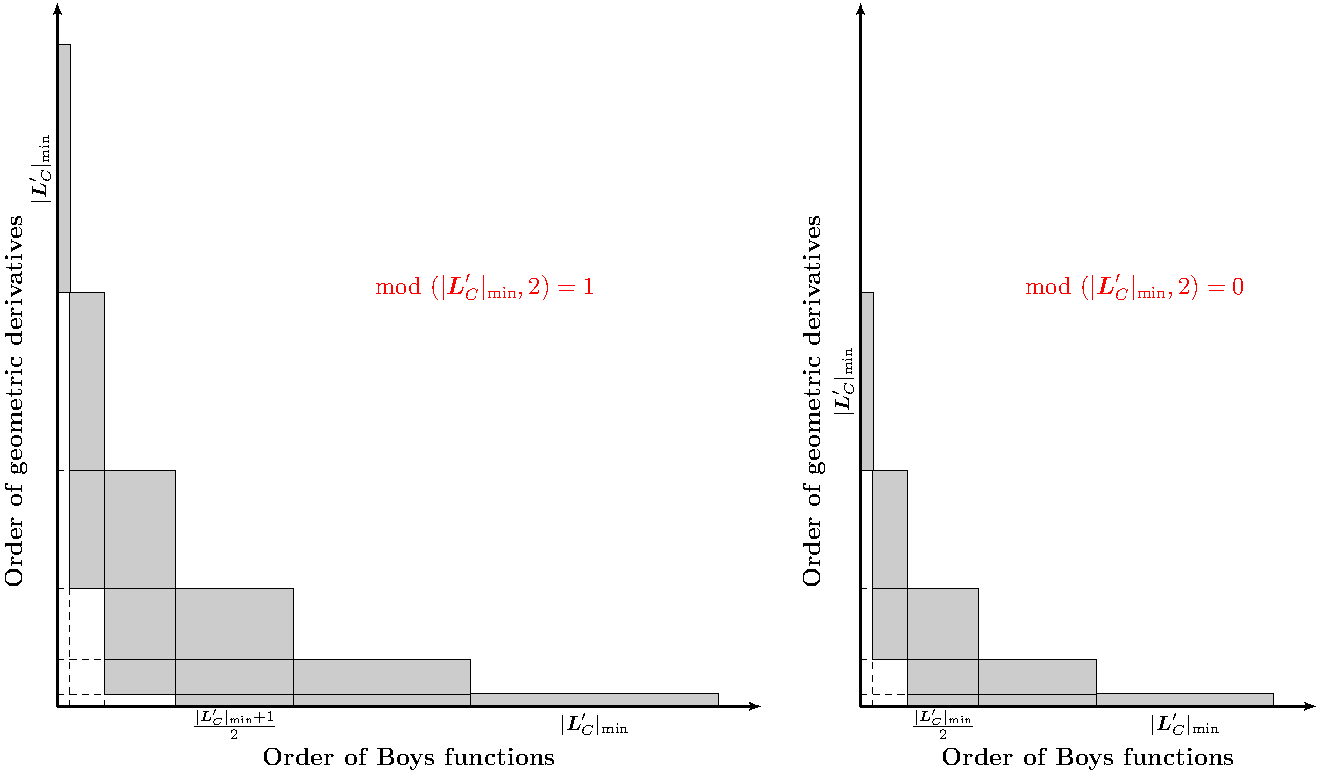
\includegraphics[width=5.5in]{nucpot_geom.pdf}
  \caption{Procedure of recurrence relation~(\ref{eq:r-1-geo-c}) for odd and even $|\boldsymbol{L}'_{C}|_{\min}$.}
  \label{fig:nucpot-nderv}
\end{figure}
Such a recurrence relation~(\ref{eq:r-1-geo-c}) has been implemented in \verb|nucpot_geom.F90|.

% inverse square distance potential
\subsection{Inverse Square Distance Potential}
\label{subsec:isdpot}

\begin{equation}
  \hat{O}_{\ell_{\beta}}^{\boldsymbol{K}_{0}\boldsymbol{L}_{0}}%
    =\bar{C}\left(\boldsymbol{\partial}_{\boldsymbol{M}}^{\boldsymbol{L}_{M}}\boldsymbol{r}_{M}^{\boldsymbol{m}}\right)%
      \left(\boldsymbol{\partial}_{\boldsymbol{C}}^{\boldsymbol{L}_{C}}r_{C}^{-2}\right)%
      \boldsymbol{\partial}_{\boldsymbol{r}}^{\boldsymbol{n}}
\end{equation}

% Gaussian charge potential
\subsection{Gaussian Charge Potential}
\label{subsec:gaupot}

The operator involved in Gaussian charge potential is
\begin{align}
  \hat{O}_{\ell_{\beta}}^{\boldsymbol{K}_{0}\boldsymbol{L}_{0}}%
  &=\bar{C}\left(\boldsymbol{\partial}_{\boldsymbol{M}}^{\boldsymbol{L}_{M}}\boldsymbol{r}_{M}^{\boldsymbol{m}}\right)%
    \left[\boldsymbol{\partial}_{\boldsymbol{C}}^{\boldsymbol{L}_{C}}\frac{\mathrm{erf}\left(\sqrt{\varrho}r_{C}\right)}{r_{C}}\right]%
    \boldsymbol{\partial}_{\boldsymbol{r}}^{\boldsymbol{n}}\\
  &=\frac{(-1)^{|\boldsymbol{L}_{M}|}\boldsymbol{m}!}{(\boldsymbol{m}-\boldsymbol{L}_{M})!}%
    \bar{C}(-2b_{j\lambda})^{|\boldsymbol{n}|}%
    \boldsymbol{r}_{M}^{\boldsymbol{m}-\boldsymbol{L}_{M}}%
    \left[\boldsymbol{\partial}_{\boldsymbol{C}}^{\boldsymbol{L}_{C}}\frac{\mathrm{erf}\left(\sqrt{\varrho}r_{C}\right)}{r_{C}}\right]%
    \frac{\boldsymbol{\partial}_{\boldsymbol{R}_{\lambda}}^{\boldsymbol{l}_{\lambda}}}%
      {(2b_{j\lambda})^{|\boldsymbol{l}_{\lambda}|}},\nonumber
\end{align}
such that
\begin{align}
  \left[\boldsymbol{l}_{\kappa}\boldsymbol{l}_{\lambda}\boldsymbol{L}_{C}%
    \boldsymbol{L}_{M}\boldsymbol{m}\boldsymbol{n}\Big|%
    \hat{O}_{\ell_{\beta}}^{\boldsymbol{K}_{0}\boldsymbol{L}_{0}}\right]_{ij}
  &=\frac{(-1)^{|\boldsymbol{L}_{M}|}\boldsymbol{m}!}{(\boldsymbol{m}-\boldsymbol{L}_{M})!}%
    \bar{C}(-2b_{j\lambda})^{|\boldsymbol{n}|}\\
  &\times\frac{\boldsymbol{\partial}_{\boldsymbol{R}_{\kappa}}^{\boldsymbol{l}_{\kappa}}}%
      {(2a_{i\kappa})^{|\boldsymbol{l}_{\kappa}|}}%
    \frac{\boldsymbol{\partial}_{\boldsymbol{R}_{\lambda}}^{\boldsymbol{l}_{\lambda}\mathrm{+}\boldsymbol{n}}}%
      {(2b_{j\lambda})^{|\boldsymbol{l}_{\lambda}|\mathrm{+}|\boldsymbol{n}|}}%
    \boldsymbol{\partial}_{\boldsymbol{C}}^{\boldsymbol{L}_{C}}%
    \left[\mathrm{e}^{-u_{ij}R_{\kappa\lambda}^2}\int%
      \frac{\boldsymbol{r}_{M}^{\boldsymbol{m}-\boldsymbol{L}_{M}}\mathrm{erf}\left(\sqrt{\varrho}r_{C}\right)}{r_{C}}%
        \mathrm{e}^{-p_{ij}r_{\gamma}^2}\mathrm{d}\boldsymbol{r}\right]\nonumber\\
  &\equiv\frac{(-1)^{|\boldsymbol{L}_{M}|}\boldsymbol{m}!}{(\boldsymbol{m}-\boldsymbol{L}_{M})!}%
    \left[\boldsymbol{l}_{\kappa},\boldsymbol{l}_{\lambda}\mathrm{+}\boldsymbol{n},%
    \boldsymbol{L}_{C},\boldsymbol{m}\mathrm{-}\boldsymbol{L}_{M};0\right]_{ij},\nonumber
\end{align}
where
\begin{equation}
  \left[\boldsymbol{l}'_{\kappa}\boldsymbol{l}'_{\lambda}\boldsymbol{L}'_{C}\boldsymbol{m}';0\right]_{ij}
  =\bar{C}(-2b_{j\lambda})^{|\boldsymbol{n}|}%
    \frac{\boldsymbol{\partial}_{\boldsymbol{R}_{\kappa}}^{\boldsymbol{l}'_{\kappa}}}%
      {(2a_{i\kappa})^{|\boldsymbol{l}'_{\kappa}|}}%
    \frac{\boldsymbol{\partial}_{\boldsymbol{R}_{\lambda}}^{\boldsymbol{l}'_{\lambda}}}%
      {(2b_{j\lambda})^{|\boldsymbol{l}'_{\lambda}|}}%
    \boldsymbol{\partial}_{\boldsymbol{C}}^{\boldsymbol{L}'_{C}}%
    \left[\mathrm{e}^{-u_{ij}R_{\kappa\lambda}^2}\int%
      \frac{\boldsymbol{r}_{M}^{\boldsymbol{m}'}\mathrm{erf}\left(\sqrt{\varrho}r_{C}\right)}{r_{C}}%
        \mathrm{e}^{-p_{ij}r_{\gamma}^2}\mathrm{d}\boldsymbol{r}\right].
\end{equation}

The evaluation of $\left[\boldsymbol{l}'_{\kappa}\boldsymbol{l}'_{\lambda}\boldsymbol{L}'_{C}\boldsymbol{m}';0\right]_{ij}$
could be performed as the case of nuclear attraction potential in Section~\ref{subsec:nucpot}, and we finally need to
consider the geometric derivatives on operator center $\boldsymbol{C}$
\begin{equation}
  \left[\boldsymbol{00}\boldsymbol{L}'_{C}\boldsymbol{0};0\right]_{ij}
  =\bar{C}(-2b_{j\lambda})^{|\boldsymbol{n}|}%
    \boldsymbol{\partial}_{\boldsymbol{C}}^{\boldsymbol{L}'_{C}}%
    \left[\mathrm{e}^{-u_{ij}R_{\kappa\lambda}^2}%
      \int\frac{\mathrm{e}^{-p_{ij}r_{\gamma}^2}\mathrm{erf}\left(\sqrt{\varrho}r_{C}\right)}{r_{C}}\mathrm{d}\boldsymbol{r}\right].
\end{equation}
By noticing that
\begin{equation}
  \mathrm{erf}\left(\sqrt{\varrho}r_{C}\right)=\frac{2}{\sqrt{\pi}}\int_{0}^{\sqrt{\varrho}r_{C}}\mathrm{e}^{-t^{2}}\mathrm{d}t,
\end{equation}
we get
\begin{equation}
  \int\frac{\mathrm{e}^{-p_{ij}r_{\gamma}^2}\mathrm{erf}\left(\sqrt{\varrho}r_{C}\right)}{r_{C}}\mathrm{d}\boldsymbol{r}
  =\frac{2\pi}{\varrho}\tilde{F}_{0}\left(\frac{p_{ij}}{\varrho},p_{ij}R_{C\gamma}^2\right),
\end{equation}
where we have introduced $(n_{0}\ge0,\tau>0,T\ge0)$
\begin{align}
  \tilde{F}_{n_{0}}\left(\tau,T\right)
  &=\int_{0}^{1}\frac{u^{2n_{0}}}{(\tau+u^{2})^{n_{0}+\frac{3}{2}}}%
    \mathrm{e}^{-T\frac{u^{2}}{\tau+u^{2}}}\mathrm{d}u\\
  &=\frac{1}{\tau\sqrt{1+\tau}(1+\tau)^{n_{0}}}F_{n_{0}}\left(\frac{T}{1+\tau}\right)\nonumber
\end{align}
with $F_{n_{0}}(T)$ being the $n_{0}$th order Boys function.

We notice the same relation of $\tilde{F}_{n_{0}}\left(\tau,T\right)$ as that of Boys function
\begin{equation}
  \boldsymbol{\partial}_{\boldsymbol{C}}^{\boldsymbol{e}_{\xi}}\tilde{F}_{n_{0}}\left(\frac{p_{ij}}{\varrho},p_{ij}R_{C\gamma}^2\right)
  =(\boldsymbol{R}_{C\gamma})_{\xi}(-2p_{ij})\tilde{F}_{n_{0}+1}\left(\frac{p_{ij}}{\varrho},p_{ij}R_{C\gamma}^2\right),
\end{equation}
so that
\begin{equation}
  \label{eq:gaupot-geo-c}
  \left[\boldsymbol{00},\boldsymbol{L}'_{C}\mathrm{+}\boldsymbol{e}_{\xi},\boldsymbol{0};n_{0}\right]_{ij}
  =(\boldsymbol{R}_{C\gamma})_{\xi}\left[\boldsymbol{00}\boldsymbol{L}'_{C}\boldsymbol{0};n_{0}\mathrm{+}1\right]_{ij}%
  +(\boldsymbol{L}'_{C})_{\xi}\left[\boldsymbol{00},\boldsymbol{L}_{C}'\mathrm{-}\boldsymbol{e}_{\xi},%
    \boldsymbol{0};n_{0}\mathrm{+}1\right]_{ij},
\end{equation}
and
\begin{align}
  \left[\boldsymbol{0000};n_{0}\right]_{ij}
  &=\bar{C}(-2b_{j\lambda})^{|\boldsymbol{n}|}\mathrm{e}^{-u_{ij}R_{\kappa\lambda}^2}%
    \frac{2\pi}{\varrho}(-2p_{ij})^{n_{0}}\tilde{F}_{n_{0}}\left(\frac{p_{ij}}{\varrho},p_{ij}R_{C\gamma}^2\right)\\
  &=\bar{C}(-2b_{j\lambda})^{|\boldsymbol{n}|}\mathrm{e}^{-u_{ij}R_{\kappa\lambda}^2}%
    \frac{2\pi}{p_{ij}}\sqrt{\frac{\varrho}{\varrho+p_{ij}}}%
    \left(-2\frac{\varrho p_{ij}}{\varrho+p_{ij}}\right)^{n_{0}}%
    F_{n_{0}}\left(\frac{\varrho p_{ij}}{\varrho+p_{ij}}R_{C\gamma}^2\right).\nonumber
\end{align}

% diamagnetic spin-orbit coupling
\subsection{Diamagnetic Spin-Orbit Coupling}
\label{subsec:dso}

\begin{equation}
  \hat{O}_{\ell_{\beta}}^{\boldsymbol{K}_{0}\boldsymbol{L}_{0}}%
    =\bar{C}\left(\boldsymbol{\partial}_{\boldsymbol{C}_{1}}^{\boldsymbol{L}_{C_{1}}}r_{C_{1}}^{-1}\right)%
      \left(\boldsymbol{\partial}_{\boldsymbol{C}_{2}}^{\boldsymbol{L}_{C_{2}}}r_{C_{2}}^{-1}\right)%
      \boldsymbol{\partial}_{\boldsymbol{r}}^{\boldsymbol{n}}
\end{equation}

% effective core potential
\subsection{Effective Core Potential}
\label{subsec:ecp}

Effective core potential
\begin{equation}
  \label{eq:ecp-op1}
  \hat{O}_{\ell_{\beta}}^{\boldsymbol{K}_{0}\boldsymbol{L}_{0}}
  =U_{L}(r_C)+\sum_{l=0}^{L-1}\sum_{m=-l}^{l}|Y_{lm}\rangle[U_l(r_C)-U_{L}(r_C)]\langle Y_{lm}|,
\end{equation}
where $Y_{lm}(\theta_C,\varphi_C)$ are real spherical harmonics centered on $\boldsymbol{C}$,
$U_L(r_C)$ and $U_l(r_C)-U_{L}(r_C)$ ($l=0,\dots,L-1$) are expressed as combinations of Gaussians
\begin{align}
  U_L(r_C)&=\frac{N_\text{core}}{r_C}+\sum_{k}d_{kL}r_{C}^{n_{kL}}\mathrm{e}^{-c_{kL}r_{C}^{2}},\\
  U_l(r_C)-U_L(r_C)&=\sum_{k}d_{kl}r_{C}^{n_{kl}}\mathrm{e}^{-c_{kl}r_{C}^{2}}.  
\end{align}

The evaluation of integral over $\frac{N_\text{core}}{r_C}$ has been discussed in our recent
work~\cite{Gao:IJQC:2010}. Therefore, the new types of integrals arising from the geometric
derivative of integral (\ref{eq:basic-int}) over the ECP operator (\ref{eq:ecp-op1}) are~\cite{McMurchie:JCP44:289,Flores-Moreno:JCC27:1009}
\begin{equation}
  \chi_{\kappa\lambda}=4\pi\int_{0}^{+\infty}\sum_{k}d_{kL}%
    \left\langle\boldsymbol{l}_{\kappa}\boldsymbol{l}_{\lambda}%
      \boldsymbol{L}_{C};n_{kL}\mathrm{+}2,0\right\rangle\mathrm{d}{r},
\end{equation}
and
\begin{equation}
  \gamma_{\kappa\lambda}=4\pi\sum_{l=0}^{L-1}\sum_{m=-l}^{l}\sum_{\mu_1,\mu_2=-l}^{l}%
    \left(\sum_{|\boldsymbol{l}_1|,|\boldsymbol{l}_2|=l}%
    u_{\boldsymbol{l}_1}^{l\mu_1}u_{\boldsymbol{l}_2}^{l\mu_2}%
    v_{\boldsymbol{l}_1}^{lm}v_{\boldsymbol{l}_2}^{lm}\right)%
    \int_{0}^{+\infty}\sum_{k}d_{kl}%
    \left\langle\boldsymbol{l}_{\kappa}\boldsymbol{l}_{\lambda}%
      \boldsymbol{L}_{C};ll,n_{kl}\mathrm{+}2\right\rangle\mathrm{d}{r},
\end{equation}
where
\begin{align}
  \left\langle\boldsymbol{l}_{\kappa}\boldsymbol{l}_{\lambda}\boldsymbol{L}_{C};nn'\right\rangle
  &=\frac{\boldsymbol{\partial}_{\boldsymbol{R}_{\kappa}}^{\boldsymbol{l}_{\kappa}}}%
      {(2a_{\kappa})^{|\boldsymbol{l}_{\kappa}|}}%
    \frac{\boldsymbol{\partial}_{\boldsymbol{R}_{\lambda}}^{\boldsymbol{l}_{\lambda}}}%
      {(2b_{\lambda})^{|\boldsymbol{l}_{\lambda}|}}%
    \boldsymbol{\partial}_{\boldsymbol{C}}^{\boldsymbol{L}_{C}}%
    \left[\mathrm{e}^{-a_{\kappa}R_{C\kappa}^{2}-b_{\lambda}R_{C\lambda}^{2}}%
    r^{n'+n}\mathrm{e}^{-\alpha_{kL}r^2}\frac{M_{n}(R_{S}r)}{(R_{S}r)^{n}}\right],\\
  \boldsymbol{R}_{S}&=-2(a_{\kappa}\boldsymbol{R}_{C\kappa}+b_{\lambda}\boldsymbol{R}_{C\lambda}),\\
  \alpha_{kL}&=a_{\kappa}+b_{\lambda}+c_{kL},
\end{align}
and
\begin{align}
%  \Omega_{l\mu,lm}^{000}
%  &=\int_{0}^{2\pi}\int_{0}^{\pi}Y_{l\mu}(\theta,\varphi)Y_{lm}(\theta,\varphi)\sin{\theta}\mathrm{d}{\theta}\mathrm{d}{\varphi},
%    \;(\mu=\mu_1\text{ or }\mu_2),\\
  \left\langle\boldsymbol{l}_{\kappa}\boldsymbol{l}_{\lambda}\boldsymbol{L}_{C};n_{1}n_{2}n'\right\rangle
  &=4\pi\frac{\boldsymbol{\partial}_{\boldsymbol{R}_{\kappa}}^{\boldsymbol{l}_{\kappa}}}%
      {(2a_{\kappa})^{|\boldsymbol{l}_{\kappa}|}}%
    \frac{\boldsymbol{\partial}_{\boldsymbol{R}_{\lambda}}^{\boldsymbol{l}_{\lambda}}}%
      {(2b_{\lambda})^{|\boldsymbol{l}_{\lambda}|}}%
    \boldsymbol{\partial}_{\boldsymbol{C}}^{\boldsymbol{L}_{C}}%
    \Bigl[\mathrm{e}^{-a_{\kappa}R_{C\kappa}^{2}-b_{\lambda}R_{C\lambda}^{2}}%
    Y_{n_{1}\mu_1}\left(\theta_{R_{S_{\kappa}}},\varphi_{R_{S_{\kappa}}}\right)\\
  &\times Y_{n_{2}\mu_2}\left(\theta_{R_{S_{\lambda}}},\varphi_{R_{S_{\lambda}}}\right)%
    r^{n'}\mathrm{e}^{-\alpha_{kl}r^2}M_{n_1}(R_{S_{\kappa}}r)M_{n_2}(R_{S_{\lambda}}r)\Bigr],\nonumber\\
  \boldsymbol{R}_{S_{\kappa}}&=-2a_{\kappa}\boldsymbol{R}_{C\kappa},\\
  \boldsymbol{R}_{S_{\lambda}}&=-2b_{\lambda}\boldsymbol{R}_{C\lambda},\\
  \alpha_{kl}&=a_{\kappa}+b_{\lambda}+c_{kl}.
\end{align}
$u_{\boldsymbol{l}_1}^{l\mu_1}$, $u_{\boldsymbol{l}_2}^{l\mu_2}$, $v_{\boldsymbol{l}_1}^{lm}$
and $v_{\boldsymbol{l}_2}^{lm}$ in the integral $\gamma_{\kappa\lambda}$ are the transform
coefficients between real spherical harmonics and unitary sphere polynomials, and could be
evaluated analytically~\cite{Flores-Moreno:JCC27:1009}.
%\fixme{\begin{align}
%  u_{\boldsymbol{l}}^{l\mu}
%    &=\sqrt{\frac{2l+1}{2\pi}\frac{(l-|\mu|)!}{(l+|\mu|)!}}\frac{1}{2^{l}l!}%
%      \sum_{i=j}^{(l-|\mu|)/2}\binom{l}{i}\binom{i}{j}\frac{(-1)^i(2l-2i)!}{(l-|\mu|-2i)!},\\
%  v_{\boldsymbol{l}}^{lm}
%    &=.
%\end{align}}

The function $M_{n}(x)$ in the integrands $\left\langle\boldsymbol{l}_{\kappa}\boldsymbol{l}_{\lambda}\boldsymbol{L}_{C};nn'\right\rangle$
and $\left\langle\boldsymbol{l}_{\kappa}\boldsymbol{l}_{\lambda}\boldsymbol{L}_{C};n_{1}n_{2}n'\right\rangle$
is a modified spherical Bessel function of the first kind
\begin{equation}
  M_{n}(x)=x^{n}\left(\frac{1}{x}\frac{\mathrm{d}}{\mathrm{d}x}\right)^{n}\frac{\sinh x}{x}.
%  =\text{i}^{n}j_{n}(-\text{i}x),
\end{equation}
%where $j_{n}(z)$ is the spherical Bessel function of the first kind.

Notice the relationship between the real solid-harmonics $S_{lm}(r,\theta,\varphi)$ and
real spherical harmonics~\cite{Helgaker:2000}
\begin{equation}
  S_{lm}(r,\theta,\varphi)=(-1)^{m}\sqrt{\frac{4\pi}{2l+1}}r^{l}Y_{lm}(\theta,\varphi),
\end{equation}
the function $\mathrm{e}^{-a_{\kappa}R_{C\kappa}^{2}}Y_{n_1\mu_1}\left(\theta_{R_{S_{\kappa}}},\varphi_{R_{S_{\kappa}}}\right)$
in the integrand $\left\langle\boldsymbol{l}_{\kappa}\boldsymbol{l}_{\lambda}\boldsymbol{L}_{C};n_{1}n_{2}n'\right\rangle$,
for instance, could be written as
\begin{align}
  \mathrm{e}^{-a_{\kappa}R_{C\kappa}^{2}}Y_{n_1\mu_1}\left(\theta_{R_{S_{\kappa}}},\varphi_{R_{S_{\kappa}}}\right)
  &=(-1)^{\mu_{1}}\sqrt{\frac{2n_{1}+1}{4\pi}}\frac{1}{R_{S_{\kappa}}^{n_{1}}}%
    S_{n_{1}\mu_{1}}(\boldsymbol{R}_{S_{\kappa}})\mathrm{e}^{-\frac{1}{4a_{\kappa}}R_{S_{\kappa}}^{2}}\\
  &=(-1)^{n_{1}+\mu_{1}}\sqrt{\frac{2n_{1}+1}{4\pi}}\frac{1}{R_{S_{\kappa}}^{n_{1}}}%
    \sum_{|\boldsymbol{n}'_{1}|=n_{1}}S_{\boldsymbol{n}'_{1}}^{n_{1}\mu_{1}}%
    \left(\boldsymbol{\partial}_{\boldsymbol{R}_{\kappa}}^{\boldsymbol{n}'_{1}}%
      \mathrm{e}^{-a_{\kappa}R_{C\kappa}^{2}}\right),\nonumber
\end{align}
where we have transformed the real solid-harmonics to the sum of Hermite Gaussians,
and $S_{\boldsymbol{n}'_{1}}^{n_{1}\mu_{1}}$ are the the transformation coefficients
between Cartesian and real solid-harmonic Gaussians~\cite{Reine:PCCP9:4771}.
Therefore, we could rewrite $\left\langle\boldsymbol{l}_{\kappa}\boldsymbol{l}_{\lambda}\boldsymbol{L}_{C};n_{1}n_{2}n'\right\rangle$ as
\begin{align}
  \left\langle\boldsymbol{l}_{\kappa}\boldsymbol{l}_{\lambda}\boldsymbol{L}_{C};n_{1}n_{2}n'\right\rangle
  &=(-1)^{n_{1}+\mu_{1}+n_{2}+\mu_{2}}\sqrt{(2n_{1}+1)(2n_{2}+1)}\\
  &\times\sum_{|\boldsymbol{n}'_{1}|=n_{1}}\sum_{|\boldsymbol{n}'_{2}|=n_{2}}%
    S_{\boldsymbol{n}'_{1}}^{n_{1}\mu_{1}}S_{\boldsymbol{n}'_{2}}^{n_{2}\mu_{2}}%
    \left\langle\boldsymbol{l}_{\kappa}\boldsymbol{l}_{\lambda}\boldsymbol{L}_{C}%
      \boldsymbol{n}'_{1}\boldsymbol{n}'_{2};n_{1}n_{2}n'\right\rangle,\nonumber
\end{align}
where
\begin{align}
  \left\langle\boldsymbol{l}_{\kappa}\boldsymbol{l}_{\lambda}\boldsymbol{L}_{C}%
    \boldsymbol{n}'_{1}\boldsymbol{n}'_{2};n_{1}n_{2}n'\right\rangle
  &=\frac{\boldsymbol{\partial}_{\boldsymbol{R}_{\kappa}}^{\boldsymbol{l}_{\kappa}}}%
      {(2a_{\kappa})^{|\boldsymbol{l}_{\kappa}|}}%
    \frac{\boldsymbol{\partial}_{\boldsymbol{R}_{\lambda}}^{\boldsymbol{l}_{\lambda}}}%
      {(2b_{\lambda})^{|\boldsymbol{l}_{\lambda}|}}%
    \boldsymbol{\partial}_{\boldsymbol{C}}^{\boldsymbol{L}_{C}}\Biggl[%
      \left(\boldsymbol{\partial}_{\boldsymbol{R}_{\kappa}}^{\boldsymbol{n}'_{1}}%
        \mathrm{e}^{-a_{\kappa}R_{C\kappa}^{2}}\right)%
    \left(\boldsymbol{\partial}_{\boldsymbol{R}_{\lambda}}^{\boldsymbol{n}'_{2}}%
      \mathrm{e}^{-b_{\lambda}R_{C\lambda}^{2}}\right)\\
  &\times r^{n'+n_1+n_2}\mathrm{e}^{-\alpha_{kl}r^2}%
    \frac{M_{n_1}(R_{S_{\kappa}}r)}{(R_{S_{\kappa}}r)^{n_1}}%
    \frac{M_{n_2}(R_{S_{\lambda}}r)}{(R_{S_{\lambda}}r)^{n_2}}\Biggr].\nonumber
\end{align}

We next discuss the evaluation of the integrands $\left\langle\boldsymbol{l}_{\kappa}\boldsymbol{l}_{\lambda}\boldsymbol{L}_{C};nn'\right\rangle$
and $\left\langle\boldsymbol{l}_{\kappa}\boldsymbol{l}_{\lambda}\boldsymbol{L}_{C}%
\boldsymbol{n}'_{1}\boldsymbol{n}'_{2};n_{1}n_{2}n'\right\rangle$. Notice that~\cite{Abramowitz:1972}
\begin{equation}
  \left(\frac{1}{x}\frac{\mathrm{d}}{\mathrm{d}{x}}\right)^{m}\frac{M_{n}(x)}{x^n}
  =\frac{M_{n+m}(x)}{x^{n+m}},
\end{equation}
we have, for instance
\begin{equation}
  \label{eq:modified-spherical-bessel-derivative}
  \boldsymbol{\partial}_{\boldsymbol{R}_{\kappa}}^{\boldsymbol{e}_{\xi}}\left[\frac{M_{n}(R_{S}r)}{(R_{S}r)^{n}}\right]
  =a_{\kappa}r^2(\boldsymbol{R}_{S})_{\xi}\frac{M_{n+1}(R_{S}r)}{(R_{S}r)^{n+1}}.
\end{equation}
The recurrence relations of $\left\langle\boldsymbol{l}_{\kappa}\boldsymbol{l}_{\lambda}\boldsymbol{L}_{C};nn'\right\rangle$
and $\left\langle\boldsymbol{l}_{\kappa}\boldsymbol{l}_{\lambda}\boldsymbol{L}_{C}%
\boldsymbol{n}'_{1}\boldsymbol{n}'_{2};n_{1}n_{2}n'\right\rangle$ could thus be obtained using
the translational invariance~\cite{Komornicki:CPL45:595,Kahn:JCP75:3962}, Eq.~(\ref{eq:r-HGTO}),
Eqs.~(\ref{eq:modified-spherical-bessel-derivative}) and (\ref{eq:multi-partial-R})
\begin{align}
  \left\langle\boldsymbol{l}_{\kappa}\boldsymbol{l}_{\lambda},%
    \boldsymbol{L}_{C}\mathrm{+}\boldsymbol{e}_{\xi};nn'\right\rangle
  &=-2a_{\kappa}\left\langle\boldsymbol{l}_{\kappa}\mathrm{+}\boldsymbol{e}_{\xi},%
    \boldsymbol{l}_{\lambda}\boldsymbol{L}_{C};nn'\right\rangle%
  -2b_{\lambda}\left\langle\boldsymbol{l}_{\kappa},%
    \boldsymbol{l}_{\lambda}\mathrm{+}\boldsymbol{e}_{\xi},\boldsymbol{L}_{C};nn'\right\rangle,
\end{align}
%
\begin{align}
  \left\langle\boldsymbol{l}_{\kappa}\mathrm{+}\boldsymbol{e}_{\xi},%
    \boldsymbol{l}_{\lambda}\boldsymbol{L}_{C};nn'\right\rangle
  =\,&\left\langle\boldsymbol{l}_{\kappa},%
    \boldsymbol{l}_{\lambda}\mathrm{+}\boldsymbol{e}_{\xi},\boldsymbol{L}_{C};nn'\right\rangle
  -(\boldsymbol{R}_{\kappa\lambda})_{\xi}%
    \left\langle\boldsymbol{l}_{\kappa}\boldsymbol{l}_{\lambda}\boldsymbol{L}_{C};nn'\right\rangle\\
  &-\frac{(\boldsymbol{l}_{\kappa})_{\xi}}{2a_{\kappa}}%
    \left\langle\boldsymbol{l}_{\kappa}\mathrm{-}\boldsymbol{e}_{\xi},%
    \boldsymbol{l}_{\lambda}\boldsymbol{L}_{C};nn'\right\rangle
  +\frac{(\boldsymbol{l}_{\lambda})_{\xi}}{2b_{\lambda}}%
    \left\langle\boldsymbol{l}_{\kappa},\boldsymbol{l}_{\lambda}\mathrm{-}\boldsymbol{e}_{\xi},%
    \boldsymbol{L}_{C};nn'\right\rangle,\nonumber
\end{align}
%
\begin{align}
  \left\langle\boldsymbol{l}_{\kappa},%
    \boldsymbol{l}_{\lambda}\mathrm{+}\boldsymbol{e}_{\xi},\boldsymbol{L}_{C};nn'\right\rangle
  =\,&(\boldsymbol{R}_{C\lambda})_{\xi}%
    \left\langle\boldsymbol{l}_{\kappa}\boldsymbol{l}_{\lambda}\boldsymbol{L}_{C};nn'\right\rangle
  -\frac{(\boldsymbol{l}_{\lambda})_{\xi}}{2b_{\lambda}}%
    \left\langle\boldsymbol{l}_{\kappa},%
    \boldsymbol{l}_{\lambda}\mathrm{-}\boldsymbol{e}_{\xi},\boldsymbol{L}_{C};nn'\right\rangle\\
  &+(\boldsymbol{L}_{C})_{\xi}%
    \left\langle\boldsymbol{l}_{\kappa}\boldsymbol{l}_{\lambda},%
    \boldsymbol{L}_{C}\mathrm{-}\boldsymbol{e}_{\xi};nn'\right\rangle%
  +\frac{(\boldsymbol{R}_S)_{\xi}}{2}%
    \left\langle\boldsymbol{l}_{\kappa}\boldsymbol{l}_{\lambda}%
      \boldsymbol{L}_{C};n\mathrm{+}1,n'\mathrm{+}1\right\rangle\nonumber\\
  &+\frac{(\boldsymbol{l}_{\kappa})_{\xi}}{2}%
    \left\langle\boldsymbol{l}_{\kappa}\mathrm{-}\boldsymbol{e}_{\xi},\boldsymbol{l}_{\lambda}%
      \boldsymbol{L}_{C};n\mathrm{+}1,n'\mathrm{+}1\right\rangle
  +\frac{(\boldsymbol{l}_{\lambda})_{\xi}}{2}%
    \left\langle\boldsymbol{l}_{\kappa},\boldsymbol{l}_{\lambda}\mathrm{-}\boldsymbol{e}_{\xi},%
      \boldsymbol{L}_{C};n\mathrm{+}1,n'\mathrm{+}1\right\rangle\nonumber\\
  &-(\boldsymbol{L}_{C})_{\xi}(a_{\kappa}+b_{\lambda})%
    \left\langle\boldsymbol{l}_{\kappa}\boldsymbol{l}_{\lambda},%
      \boldsymbol{L}_{C}\mathrm{-}\boldsymbol{e}_{\xi};n\mathrm{+}1,n'\mathrm{+}1\right\rangle,\nonumber
\end{align}
and
\begin{align}
  \left\langle\boldsymbol{l}_{\kappa}\boldsymbol{l}_{\lambda},%
    \boldsymbol{L}_{C}\mathrm{+}\boldsymbol{e}_{\xi},%
    \boldsymbol{n}'_{1}\boldsymbol{n}'_{2};n_{1}n_{2}n'\right\rangle
  =\,&-2a_{\kappa}\left\langle\boldsymbol{l}_{\kappa}\mathrm{+}\boldsymbol{e}_{\xi},%
    \boldsymbol{l}_{\lambda}\boldsymbol{L}_{C}%
    \boldsymbol{n}'_{1}\boldsymbol{n}'_{2};n_{1}n_{2}n'\right\rangle\\
  &-2b_{\lambda}\left\langle\boldsymbol{l}_{\kappa},%
    \boldsymbol{l}_{\lambda}\mathrm{+}\boldsymbol{e}_{\xi},%
    \boldsymbol{L}_{C}\boldsymbol{n}'_{1}\boldsymbol{n}'_{2};n_{1}n_{2}n'\right\rangle,\nonumber
\end{align}
%
\begin{align}
  \left\langle\boldsymbol{l}_{\kappa}\mathrm{+}\boldsymbol{e}_{\xi},%
    \boldsymbol{l}_{\lambda}\boldsymbol{L}_{C}%
    \boldsymbol{n}'_{1}\boldsymbol{n}'_{2};n_{1}n_{2}n'\right\rangle
  =\,&\frac{1}{2a_{\kappa}}%
    \left\langle\boldsymbol{l}_{\kappa}\boldsymbol{l}_{\lambda}\boldsymbol{L}_{C},%
    \boldsymbol{n}'_{1}\mathrm{+}\boldsymbol{e}_{\xi},\boldsymbol{n}'_{2};n_{1}n_{2}n'\right\rangle\\
  &+\frac{(\boldsymbol{R}_{S_{\kappa}})_{\xi}}{2}%
    \left\langle\boldsymbol{l}_{\kappa}\boldsymbol{l}_{\lambda}\boldsymbol{L}_{C}%
    \boldsymbol{n}'_{1}\boldsymbol{n}'_{2};n_{1}\mathrm{+}1,n_{2},n'\mathrm{+}1\right\rangle\nonumber\\
  &+(\boldsymbol{l}_{\kappa})_{\xi}%
    \left\langle\boldsymbol{l}_{\kappa}\mathrm{-}\boldsymbol{e}_{\xi},\boldsymbol{l}_{\lambda}\boldsymbol{L}_{C}%
    \boldsymbol{n}'_{1}\boldsymbol{n}'_{2};n_{1}\mathrm{+}1,n_{2},n'\mathrm{+}1\right\rangle\nonumber\\
  &-2a_{\kappa}(\boldsymbol{L}_{C})_{\xi}%
    \left\langle\boldsymbol{l}_{\kappa}\boldsymbol{l}_{\lambda},\boldsymbol{L}_{C}\mathrm{-}\boldsymbol{e}_{\xi},%
    \boldsymbol{n}'_{1}\boldsymbol{n}'_{2};n_{1}\mathrm{+}1,n_{2},n'\mathrm{+}1\right\rangle,\nonumber
\end{align}
%
\begin{align}
  \left\langle\boldsymbol{l}_{\kappa},\boldsymbol{l}_{\lambda}\mathrm{+}\boldsymbol{e}_{\xi},%
    \boldsymbol{L}_{C}\boldsymbol{n}'_{1}\boldsymbol{n}'_{2};n_{1}n_{2}n'\right\rangle
  =\,&\frac{1}{2b_{\lambda}}%
    \left\langle\boldsymbol{l}_{\kappa}\boldsymbol{l}_{\lambda}\boldsymbol{L}_{C},%
    \boldsymbol{n}'_{1},\boldsymbol{n}'_{2}\mathrm{+}\boldsymbol{e}_{\xi};n_{1}n_{2}n'\right\rangle\\
  &+\frac{(\boldsymbol{R}_{S_{\lambda}})_{\xi}}{2}%
    \left\langle\boldsymbol{l}_{\kappa}\boldsymbol{l}_{\lambda}\boldsymbol{L}_{C}%
    \boldsymbol{n}'_{1}\boldsymbol{n}'_{2};n_{1},n_{2}\mathrm{+}1,n'\mathrm{+}1\right\rangle\nonumber\\
  &+(\boldsymbol{l}_{\lambda})_{\xi}%
    \left\langle\boldsymbol{l}_{\kappa},\boldsymbol{l}_{\lambda}\mathrm{-}\boldsymbol{e}_{\xi},\boldsymbol{L}_{C}%
    \boldsymbol{n}'_{1}\boldsymbol{n}'_{2};n_{1},n_{2}\mathrm{+}1,n'\mathrm{+}1\right\rangle\nonumber\\
  &-2b_{\lambda}(\boldsymbol{L}_{C})_{\xi}%
    \left\langle\boldsymbol{l}_{\kappa}\boldsymbol{l}_{\lambda},\boldsymbol{L}_{C}\mathrm{-}\boldsymbol{e}_{\xi},%
    \boldsymbol{n}'_{1}\boldsymbol{n}'_{2};n_{1},n_{2}\mathrm{+}1,n'\mathrm{+}1\right\rangle,\nonumber
\end{align}
%
\begin{align}
  \left\langle\boldsymbol{l}_{\kappa}\boldsymbol{l}_{\lambda}\boldsymbol{L}_{C},%
    \boldsymbol{n}'_{1}\mathrm{+}\boldsymbol{e}_{\xi},\boldsymbol{n}'_{2};n_{1}n_{2}n'\right\rangle
  =\,&2a_{\kappa}(\boldsymbol{R}_{C\kappa})_{\xi}%
    \left\langle\boldsymbol{l}_{\kappa}\boldsymbol{l}_{\lambda}\boldsymbol{L}_{C}%
    \boldsymbol{n}'_{1}\boldsymbol{n}'_{2};n_{1}n_{2}n'\right\rangle\\
  &-(\boldsymbol{l}_{\kappa})_{\xi}%
    \left\langle\boldsymbol{l}_{\kappa}\mathrm{-}\boldsymbol{e}_{\xi},\boldsymbol{l}_{\lambda}\boldsymbol{L}_{C}%
    \boldsymbol{n}'_{1}\boldsymbol{n}'_{2};n_{1}n_{2}n'\right\rangle\nonumber\\
  &+2(\boldsymbol{L}_{C})_{\xi}a_{\kappa}%
    \left\langle\boldsymbol{l}_{\kappa}\boldsymbol{l}_{\lambda},\boldsymbol{L}_{C}\mathrm{-}\boldsymbol{e}_{\xi},%
    \boldsymbol{n}'_{1}\boldsymbol{n}'_{2};n_{1}n_{2}n'\right\rangle\nonumber\\
  &-2(\boldsymbol{n}'_{1})_{\xi}a_{\kappa}%
    \left\langle\boldsymbol{l}_{\kappa}\boldsymbol{l}_{\lambda}\boldsymbol{L}_{C},%
    \boldsymbol{n}'_{1}\mathrm{-}\boldsymbol{e}_{\xi},\boldsymbol{n}'_{2};n_{1}n_{2}n'\right\rangle,\nonumber
\end{align}
%
\begin{align}
  \left\langle\boldsymbol{l}_{\kappa}\boldsymbol{l}_{\lambda}\boldsymbol{L}_{C},%
    \boldsymbol{n}'_{1},\boldsymbol{n}'_{2}\mathrm{+}\boldsymbol{e}_{\xi};n_{1}n_{2}n'\right\rangle
  =\,&2b_{\lambda}(\boldsymbol{R}_{C\lambda})_{\xi}%
    \left\langle\boldsymbol{l}_{\kappa}\boldsymbol{l}_{\lambda}\boldsymbol{L}_{C}%
    \boldsymbol{n}'_{1}\boldsymbol{n}'_{2};n_{1}n_{2}n'\right\rangle\\
  &-(\boldsymbol{l}_{\lambda})_{\xi}%
    \left\langle\boldsymbol{l}_{\kappa},\boldsymbol{l}_{\lambda}\mathrm{-}\boldsymbol{e}_{\xi},\boldsymbol{L}_{C}%
    \boldsymbol{n}'_{1}\boldsymbol{n}'_{2};n_{1}n_{2}n'\right\rangle\nonumber\\
  &+2(\boldsymbol{L}_{C})_{\xi}b_{\lambda}%
    \left\langle\boldsymbol{l}_{\kappa}\boldsymbol{l}_{\lambda},\boldsymbol{L}_{C}\mathrm{-}\boldsymbol{e}_{\xi},%
    \boldsymbol{n}'_{1}\boldsymbol{n}'_{2};n_{1}n_{2}n'\right\rangle\nonumber\\
  &-2(\boldsymbol{n}'_{2})_{\xi}b_{\lambda}%
    \left\langle\boldsymbol{l}_{\kappa}\boldsymbol{l}_{\lambda}\boldsymbol{L}_{C},%
    \boldsymbol{n}'_{1},\boldsymbol{n}'_{2}\mathrm{-}\boldsymbol{e}_{\xi};n_{1}n_{2}n'\right\rangle.\nonumber
\end{align}

The integrals $\chi_{\kappa\lambda}$ and $\gamma_{\kappa\lambda}$ could finally be evaluated
using adaptive quadrature with the knowledge of the values of integrands
\begin{align}
  \left\langle\boldsymbol{000};nn'\right\rangle
  &=\mathrm{e}^{-a_{\kappa}R_{C\kappa}^{2}-b_{\lambda}R_{C\lambda}^{2}}%
    r^{n'+n}\mathrm{e}^{-\alpha_{kL}r^2}\frac{M_{n}(R_{S}r)}{(R_{S}r)^{n}}\\
  &=\frac{r^{n'}\left(R_{S}^{-1}\right)^{n}}%
    {\mathrm{e}^{a_{\kappa}(r-R_{C\kappa})^2+b_{\lambda}(r-R_{C\lambda})^2+c_{kL}r^2}%
      \mathrm{e}^{(R_{S_{\kappa}}+R_{S_{\lambda}}-R_{S})r}}%
    M_{n}(R_{S}r)\mathrm{e}^{-R_{S}r}\nonumber
\end{align}
and
\begin{align}
  \left\langle\boldsymbol{00000};n_{1}n_{2}n'\right\rangle
  &=\mathrm{e}^{-a_{\kappa}R_{C\kappa}^{2}-b_{\lambda}R_{C\lambda}^{2}}%
    r^{n'+n_1+n_2}\mathrm{e}^{-\alpha_{kl}r^2}%
    \frac{M_{n_1}(R_{S_{\kappa}}r)}{(R_{S_{\kappa}}r)^{n_1}}%
    \frac{M_{n_2}(R_{S_{\lambda}}r)}{(R_{S_{\lambda}}r)^{n_2}}\\
  &=\frac{r^{n'}\left(R_{S_{\kappa}}^{-1}\right)^{n_1}\left(R_{S_{\lambda}}^{-1}\right)^{n_2}}%
    {\mathrm{e}^{a_{\kappa}(r-R_{C\kappa})^2+b_{\lambda}(r-R_{C\lambda})^2+c_{kl}r^2}}%
    M_{n_1}(R_{S_{\kappa}}r)\mathrm{e}^{-R_{S_{\kappa}}r}%
    M_{n_2}(R_{S_{\lambda}}r)\mathrm{e}^{-R_{S_{\lambda}}r}\nonumber
\end{align}
at quadrature points~\cite{Flores-Moreno:JCC27:1009}. The evaluation of the scaled modified
spherical Bessel function of the first kind $M_{n}(z)\mathrm{e}^{-z}$ has been discussed
in Ref.~\cite{Flores-Moreno:JCC27:1009}.

% model core potential (Version 1)
\subsection{Model Core Potential (Version 1)}
\label{subsec:mcp1}

Model core potential (Version 1)
\begin{equation}
  \label{eq:mcp-op1}
  \hat{O}_{\ell_{\beta}}^{\boldsymbol{K}_{0}\boldsymbol{L}_{0}}
  =V_\text{mp}(r_C)+\hat{\Omega},
\end{equation}
where
\begin{equation}
  \label{eq:V-core}
  V_\text{mp}(r_C)=-\frac{Z-N_\text{core}}{r_C}\sum_{l}A_{l}r_{C}^{n_l}\mathrm{e}^{-\alpha_{l}r_{C}^{2}},
\end{equation}
and
\begin{equation}
  \label{eq:shift-op}
  \hat{\Omega}
  =-\sum_{k}f_k\epsilon_k\left|\varphi_k(\boldsymbol{r}_C)\right\rangle\left\langle\varphi_k(\boldsymbol{r}_C)\right|,
\end{equation}
with $1\le f_k\le 2$ being adjustable parameters, and $\epsilon_k$ the eigenvalue of the
$k$'th core orbital. $\varphi_k(\boldsymbol{r}_C)$ is the $k$'th core orbital,
represented by real solid-harmonic Gaussian functions.

% overlap distribution
\subsection{Overlap Distribution}
\label{subsec:odist}

Starting from Eq.~(\ref{eq:oneint-binom}), we could get the total and/or partial derivatives (evaluated
at zero fields) of overlap distribution of two contracted rotational LAOs (\ref{eq:LAO}) as

\begin{align}
  \Omega_{\kappa\lambda}(\boldsymbol{r})
  &=\sum_{\boldsymbol{K}'=\boldsymbol{0}}^{\boldsymbol{K}}%
    \sum_{\boldsymbol{L}'=\boldsymbol{0}}^{\boldsymbol{L}}%
    \binom{\boldsymbol{K}}{\boldsymbol{K}'}%
    \binom{\boldsymbol{L}}{\boldsymbol{L}'}%
    \prod^{N_{g}}\boldsymbol{\partial}_{\boldsymbol{R}_{g}}^{\boldsymbol{L}_{g}}%
    \biggl\{\boldsymbol{\partial}_{\boldsymbol{R}_{\kappa}}^{\boldsymbol{L}_{\kappa}}%
      \left[\boldsymbol{\partial}_{\boldsymbol{B}}^{\boldsymbol{K}_{1}+\boldsymbol{K}'}%
        \boldsymbol{\partial}_{\boldsymbol{J}}^{\boldsymbol{L}_{1}+\boldsymbol{L}'}%
        \omega_{\kappa}^\ast(\boldsymbol{r};\boldsymbol{B},%
          \boldsymbol{J})\right]_{\boldsymbol{B},\boldsymbol{J}=\boldsymbol{0}}\\
  &\times\boldsymbol{\partial}_{\boldsymbol{R}_{\lambda}}^{\boldsymbol{L}_{\lambda}}%
      \left[\boldsymbol{\partial}_{\boldsymbol{B}}^{\boldsymbol{K}_{2}+\boldsymbol{K}''}%
        \boldsymbol{\partial}_{\boldsymbol{J}}^{\boldsymbol{L}_{2}+\boldsymbol{L}''}%
        \omega_{\lambda}(\boldsymbol{r};\boldsymbol{B},\boldsymbol{J})\right]_{\boldsymbol{B},\boldsymbol{J}=\boldsymbol{0}}\biggr\},\nonumber\\
%
  &=\sum_{\boldsymbol{K}'=\boldsymbol{0}}^{\boldsymbol{K}}%
    \sum_{\boldsymbol{L}'=\boldsymbol{0}}^{\boldsymbol{L}}
    \binom{\boldsymbol{K}}{\boldsymbol{K}'}%
    \binom{\boldsymbol{L}}{\boldsymbol{L}'}%
    \prod^{N_{g}}\boldsymbol{\partial}_{\boldsymbol{R}_{g}}^{\boldsymbol{L}_{g}}%
    \left(\tfrac{\text{i}}{2}\right)^{|\boldsymbol{K}_{1}|+|\boldsymbol{K}'|}%
    \left(-\text{i}\right)^{|\boldsymbol{L}_{1}|+|\boldsymbol{L}'|}%
    \left(-\tfrac{\text{i}}{2}\right)^{|\boldsymbol{K}_{2}|+|\boldsymbol{K}''|}%
    \text{i}^{|\boldsymbol{L}_{2}|+|\boldsymbol{L}''|}\nonumber\\
  &\times\boldsymbol{\partial}_{\boldsymbol{R}_{\kappa}}^{\boldsymbol{L}_{\kappa}}%
    \boldsymbol{\partial}_{\boldsymbol{R}_{\lambda}}^{\boldsymbol{L}_{\lambda}}%
    \Bigl\{(\boldsymbol{R}_{\kappa G}\times\boldsymbol{r}_{P})^{\boldsymbol{K}_{1}+\boldsymbol{K}'}%
    \left[\mathbf{I}^{-T}(\boldsymbol{R}_{\kappa O}\times\boldsymbol{r}_{P})\right]^{\boldsymbol{L}_{1}+\boldsymbol{L}'}%
    \chi_{\kappa}(\boldsymbol{r})\nonumber\\
  &\times(\boldsymbol{R}_{\lambda G}\times\boldsymbol{r}_{P})^{\boldsymbol{K}_{2}+\boldsymbol{K}''}%
    \left[\mathbf{I}^{-T}(\boldsymbol{R}_{\lambda O}\times\boldsymbol{r}_{P})\right]^{\boldsymbol{L}_{2}+\boldsymbol{L}''}%
    \chi_{\lambda}(\boldsymbol{r})\Bigr\},\nonumber
\end{align}
which, by applying the recurrence relations~(\ref{eq:recurrence-mag-bra})-(\ref{eq:recurrence-phase-herm-ket}),
could be obtained from the product of two Hermite Gaussians 
\begin{equation}
  \left[\boldsymbol{l}_{\kappa}\boldsymbol{l}_{\lambda}\Big|\Omega\right]_{ij}
  =\frac{\boldsymbol{\partial}_{\boldsymbol{R}_{\kappa}}^{\boldsymbol{l}_{\kappa}}}%
      {(2a_{i\kappa})^{|\boldsymbol{l}_{\kappa}|}}%
    \frac{\boldsymbol{\partial}_{\boldsymbol{R}_{\lambda}}^{\boldsymbol{l}_{\lambda}}}%
      {(2b_{j\lambda})^{|\boldsymbol{l}_{\lambda}|}}%
    \left[\exp(-a_{i\kappa}r_{\kappa}^2)\exp(-b_{j\lambda}r_{\lambda}^2)\right]%
  =H_{i\kappa}^{\boldsymbol{l}_{\kappa}}(\boldsymbol{r})H_{j\lambda}^{\boldsymbol{l}_{\lambda}}(\boldsymbol{r}).
\end{equation}

The recurrence relations of $H_{i\kappa}^{\boldsymbol{l}_{\kappa}}(\boldsymbol{r})$ and
$H_{j\lambda}^{\boldsymbol{l}_{\lambda}}(\boldsymbol{r})$ are trivial~\cite{Reine:PCCP9:4771}
\begin{align}
  H_{i\kappa}^{\boldsymbol{l}_{\kappa}\mathrm{+}\boldsymbol{e}_{\xi}}(\boldsymbol{r})
  &=(\boldsymbol{r}_{\kappa})_{\xi}H_{i\kappa}^{\boldsymbol{l}_{\kappa}}(\boldsymbol{r})%
  -\frac{(\boldsymbol{l}_{\kappa})_{\xi}}{2a_{i\kappa}}%
    H_{i\kappa}^{\boldsymbol{l}_{\kappa}\mathrm{-}\boldsymbol{e}_{\xi}}(\boldsymbol{r}),\\
  H_{j\lambda}^{\boldsymbol{l}_{\lambda}\mathrm{+}\boldsymbol{e}_{\xi}}(\boldsymbol{r})
  &=(\boldsymbol{r}_{\lambda})_{\xi}H_{j\lambda}^{\boldsymbol{l}_{\lambda}}(\boldsymbol{r})%
  -\frac{(\boldsymbol{l}_{\lambda})_{\xi}}{2b_{j\lambda}}%
    H_{j\lambda}^{\boldsymbol{l}_{\lambda}\mathrm{-}\boldsymbol{e}_{\xi}}(\boldsymbol{r}),
\end{align}
which are implemented in \verb|prim_hgto_odist.F90| by starting from
\begin{equation}
  H_{i\kappa}^{\boldsymbol{0}}(\boldsymbol{r})H_{j\lambda}^{\boldsymbol{0}}(\boldsymbol{r})%
    =\exp(-a_{i\kappa}r_{\kappa}^2)\exp(-b_{j\lambda}r_{\lambda}^2).
\end{equation}

The value of individual HGTOs could also be easily evaluated from above recurrence relation,
which is implemented in \verb|prim_hgto_value.F90|.

% quadrature
\section{Quadrature in \textsc{Gen1Int}}
\label{sect:quadrature}

\fixme{Quadrature is used by diamagnetic spin-orbit coupling, and effective core potential ...}

% basis sets
\section{Basis Sets in \textsc{Gen1Int}}
\label{sect:basis}

% normalization of SGTOs
\subsection{Normalization of Contracted Spherical Gaussians}
\label{subsec:norm-sgto}

\fixme{Change the notations later on and adds a table for the subroutine ...}

\begin{equation}
  \chi_{\kappa}(\boldsymbol{r})=\theta_{\kappa}(\boldsymbol{r}_{\kappa})\rho_{\kappa}(r_{\kappa}),
\end{equation}
where $\rho_{\kappa}(r_{\kappa})$ is a contracted Gaussian
\begin{equation}
  \rho_{\kappa}(r_{\kappa})=\sum_{i}w_{i\kappa}\exp(-a_{i\kappa}r_{\kappa}^{2}),
\end{equation}

This section mainly follows the book~\cite{Helgaker:2000}. We rewrite the spherical Gaussian as
\begin{align}
  \chi_{\alpha_{nl}lm}&=R_{\alpha_{nl}l}(r)Y_{lm}(\theta,\phi),\\
  R_{\alpha_{nl}l}(r)&=N_{\alpha_{nl}l}(\sqrt{2\alpha_{nl}}r)^{l}\exp(-\alpha_{nl}r^2),
\end{align}
where $R_{\alpha_{nl}l}(r)$ is the radial function. $Y_{lm}$ are spherical-harmonic
angular functions, with $l$ and $m$ the total- and $z$-projected angular momentum quantum numbers,
respectively
\begin{equation}
    Y_{lm}(\theta,\phi)=\sqrt{\frac{2l+1}{4\pi}\frac{(l-m)!}{(l+m)!}}P_{l}^{m}(\cos{\theta})\exp(\text{i}m\phi)
\end{equation}
which are orthonormal
\begin{equation}
  \int_{\theta=0}^{\pi}\int_{\phi=0}^{2\pi}Y_{lm}Y_{l'm'}^{*}\sin{\theta}\mathrm{d}\theta\mathrm{d}\phi=\delta_{ll'}\delta_{mm'}, 
\end{equation}

The complex solid harmonics in Racah's normalization
\begin{equation}
    C_{lm}(r,\theta,\phi)=\sqrt{\frac{4\pi}{2l+1}}r^{l}Y_{lm}(\theta,\phi),
\end{equation}
and
\begin{equation}
    \int_{\theta=0}^{\pi}\int_{\phi=0}^{2\pi}C_{lm}C_{lm}^{*}\sin{\theta}\mathrm{d}\theta\mathrm{d}\phi=\frac{4\pi}{2l+1}r^{2l} 
\end{equation}


The following expression defines the real-valued solid harmonics
\begin{equation}
  \begin{pmatrix}
    S_{lm}\\
    S_{l,-m}
  \end{pmatrix}
  =\frac{1}{\sqrt{2}}
    \begin{pmatrix}
      (-1)^m & 1\\
      -(-1)^m\text{i} & \text{i}
    \end{pmatrix}
    \begin{pmatrix}
      C_{lm}\\
      C_{l,-m}
    \end{pmatrix},
    \qquad m>0,
\end{equation}
and for $m=0$
\begin{equation}
  S_{l0}=C_{l0}. 
\end{equation}

Therefore, the normalization constant of real-valued solid harmonics is $\frac{1}{2}\sqrt{\frac{2l+1}{\pi}}$.

The normalization constant $N_{\alpha_{nl}l}$ is
\begin{equation}
  N_{\alpha_{nl}l}=\frac{2(2\alpha_{nl})^{3/4}}{\pi^{1/4}}\sqrt{\frac{2^{l}}{(2l+1)!!}}.
\end{equation}

For contracted spherical Gaussians, we have
\begin{equation}
  R_{l}^\text{contr}(r)=\sum_{\alpha_{nl}}N_{\alpha_{nl}l}(\sqrt{2\alpha_{nl}}r)^{l}C(\alpha_{nl})\exp(-\alpha_{nl}r^2),
\end{equation}
where the summation runs over the set of (primitive) Gaussian exponents
$\alpha_{nl}$, and $C(\alpha_{nl})$ is the corresponding contraction coefficient.

The radial overlap between two spherical Gaussians is
\begin{equation}
  S_{\alpha_{1}\alpha_{2}l}
  =\int_{0}^{\infty}R_{\alpha_{1}l}(r)R_{\alpha_{2}l}(r)r^2\mathrm{d}r%
  =\left(\frac{\sqrt{4\alpha_{1}\alpha_{2}}}{\alpha_{1}+\alpha_{2}}\right)^{l+3/2},
\end{equation}
we then get the norm of $R_{l}^\text{contr}(r)$ as
\begin{equation}
  \sqrt{\int_{0}^{\infty}[R_{l}^\text{contr}(r)]^2r^2\mathrm{d}r}
  =\sqrt{\sum_{\alpha_{i},\alpha_{j}}C(\alpha_{i})C(\alpha_{j})%
    \left(\frac{\sqrt{4\alpha_{i}\alpha_{j}}}{\alpha_{i}+\alpha_{j}}\right)^{l+3/2}}.
\end{equation}

Therefore, the normalized radical part is
\begin{equation}
  \bar{R}_{l}^\text{contr}(r)=\sum_{\alpha_{nl}}%
  \frac{N_{\alpha_{nl}l}(\sqrt{2\alpha_{nl}}r)^{l}C(\alpha_{nl})} %
    {\sqrt{\sum_{\alpha_{i},\alpha_{j}}C(\alpha_{i})C(\alpha_{j})%
  \left(\frac{\sqrt{4\alpha_{i}\alpha_{j}}}{\alpha_{i}+\alpha_{j}}\right)^{l+3/2}}}\exp(-\alpha_{nl}r^2).
\end{equation}

In other words, the normalized contraction coefficient is
\begin{align}
  \bar{C}(\alpha_{nl})
  \label{eq:norm-SGTO}
  &=\frac{N_{\alpha_{nl}l}(\sqrt{2\alpha_{nl}})^{l}C(\alpha_{nl})} %
    {\sqrt{\sum_{\alpha_{i},\alpha_{j}}C(\alpha_{i})C(\alpha_{j})%
    \left(\frac{\sqrt{4\alpha_{i}\alpha_{j}}}{\alpha_{i}+\alpha_{j}}\right)^{l+3/2}}}\\
  &=\left(\frac{2}{\pi}\right)^{1/4}\frac{(4\alpha_{nl})^{l/2+3/4}}{\sqrt{(2l+1)!!}} %
    \frac{C(\alpha_{nl})}{\sqrt{\sum_{\alpha_{i},\alpha_{j}}C(\alpha_{i})C(\alpha_{j})%
    \left(\frac{\sqrt{4\alpha_{i}\alpha_{j}}}{\alpha_{i}+\alpha_{j}}\right)^{l+3/2}}}.
\end{align}

The normalization of contracted spherical Gaussians has been implemented in subroutine\linebreak
\verb|norm_contr_sgto|\index{\textsl{public} \texttt{norm\_contr\_sgto}}.

% normalization of CGTOs
\subsection{Normalization of Contracted Cartesian Gaussians}
\label{subsec:norm-cgto}

\fixme{Change the notations later on and adds a table for the subroutine ...}

In subroutine \verb|norm_contr_cgto|\index{\textsl{public} \texttt{norm\_contr\_cgto}}, we have provided
the normalization of contracted Cartesian Gaussians following the same procedure in \textsc{Dalton}
subroutine \verb|NRMORB| (so that the diagonal elements of overlap matrix scales as $(2l+1)!!$).
After that, the normalized contraction coefficient of contracted Cartesian Gaussians is
\begin{equation}
  \bar{C}(\alpha_{nl})=\left(\frac{1}{2\pi}\right)^{3/4}(4\alpha_{nl})^{l/2+3/4}%
    \frac{C(\alpha_{nl})}{\sqrt{\sum_{\alpha_{i},\alpha_{j}}C(\alpha_{i})C(\alpha_{j})%
    \left(\frac{\sqrt{4\alpha_{i}\alpha_{j}}}{\alpha_{i}+\alpha_{j}}\right)^{l+3/2}}},
\end{equation}
seems to replace $N_{\alpha_{nl}l}(\sqrt{2\alpha_{nl}})^{l}$ with
$(\frac{2\alpha_{nl}}{\pi})^{3/4}(4\alpha_{nl})^{l/2}$ in Eq. (\ref{eq:norm-SGTO}).

% HGTOs to SGTOs
\subsection{Transformation between Spherical and Hermite Gaussians}
\label{subsec:hgto-to-sgto}

\fixme{This section is not readable yet ...}

\fixme{Describe} subroutine \verb|hgto_to_sgto| ...

solid harmonics (or harmonic polynomials)
\begin{equation}
  \mathcal{Y}_{lm}(r,\theta,\phi)=r^{l}Y_{lm}(\theta,\phi)
\end{equation}
as the product of spherical harmonics with the monomials $r^{l}$.

Email from Andreas ...
\begin{verbatim}
They were no easy task, I remember. I think I eventually figured them out
by inspecting Mathematica's SphericalHarmonicY (t=theta, p=phi):

       Ylm(t,p) = sqrt[(2l+1)/4pi * (l-m)!/(l+m)!] Plm(cos(t)) exp(imp)

where the first factor is the normalization constant, Plm is the 
"associated Legendre function", and the replacements cos(t) => 
z/sqrt(xx+yy+zz), exp(imp) => (x+iy)^m. I've attached the Mathematica 
"notebook" I worked in back then (warning: very messy).
\end{verbatim}
and
\begin{verbatim}
There *may* be some tric involved, yes, because the spherical harmonic
polynomials satisfy
 
   (d2/dx2 + d2/dy2 + d2/dz2) r^l Ylm(r/|r|) = 0,
 
thus that contribution to <a|E_kin|b> disappears (There will still be
contributions involing the radial factor exp(-a r^2)).
\end{verbatim}

The transformation of kinetic energy integrals need special consideration ...

% HGTOs to geometric derivatives
\subsection{Recovering Partial Geometric Derivatives from Hermite Gaussians}
\label{subsec:hgto-to-geo}

\fixme{Describe} how to perform Eqs.~(\ref{eq:recurrence-geo-herm-bra}) and (\ref{eq:recurrence-geo-herm-ket}) as ...
\begin{align}
  \left\{\boldsymbol{L}_{\kappa}\boldsymbol{l}_{\kappa}\right\}_{\boldsymbol{K}_{0}\boldsymbol{L}_{0}/ij,\text{Herm}}
  &=(2a_{i\kappa})^{|\boldsymbol{L}_{\kappa}|}%
    \{\boldsymbol{0},\boldsymbol{l}_{\kappa}\mathrm{+}\boldsymbol{L}_{\kappa}\}_{\boldsymbol{K}_{0}\boldsymbol{L}_{0}/ij,\text{Herm}},\\
%
  \left\{\boldsymbol{L}_{\lambda}\boldsymbol{l}_{\lambda}\right\}_{\boldsymbol{K}_{0}\boldsymbol{L}_{0}/ij,\text{Herm}}
  &=(2b_{j\lambda})^{|\boldsymbol{L}_{\lambda}|}%
    \{\boldsymbol{0},\boldsymbol{l}_{\lambda}\mathrm{+}\boldsymbol{L}_{\lambda}\}_{\boldsymbol{K}_{0}\boldsymbol{L}_{0}/ij,\text{Herm}}.
\end{align}

% HGTOs to CGTOs
\subsection{Transformation between Cartesian and Hermite Gaussians}
\label{subsec:hgto-to-cgto}

The integrals using primitive Cartesian Gaussians (\ref{eq:prim-cgto-ints}) could be
recovered using Eqs.~(\ref{eq:recurrence-angular-cart-bra}) and (\ref{eq:recurrence-angular-cart-ket}),
which could be written as the following general form
\begin{equation}
 \{\boldsymbol{i}\mathrm{+}\boldsymbol{e}_{\xi},\boldsymbol{j}\}%
   =a\left(\{\boldsymbol{i},\boldsymbol{j}\mathrm{+}\boldsymbol{e}_{\xi}\}%
    +\boldsymbol{i}_{\xi}\{\boldsymbol{i}\mathrm{-}\boldsymbol{e}_{\xi},\boldsymbol{j}\}\right).
\end{equation}

The procedure of evaluating the above recurrence relation is given in Fig.~\ref{fig:hgto-to-cgto}, in which
(\textit{a}) describes the procedure of returning a specific order Cartesian and Hermite Gaussians (geometric
derivative), while (\textit{b}) depicts the procedure for a range of orders of Cartesian and Hermite Gaussians.
These two different procedures are respectively used for non London atomic orbitals (non-LAOs) and LAOs,
and implemented in files \verb|hgto_to_cgto.F90| and \verb|hgto_to_lcgto.F90|.
\begin{figure}[hbtp]
  \centering
  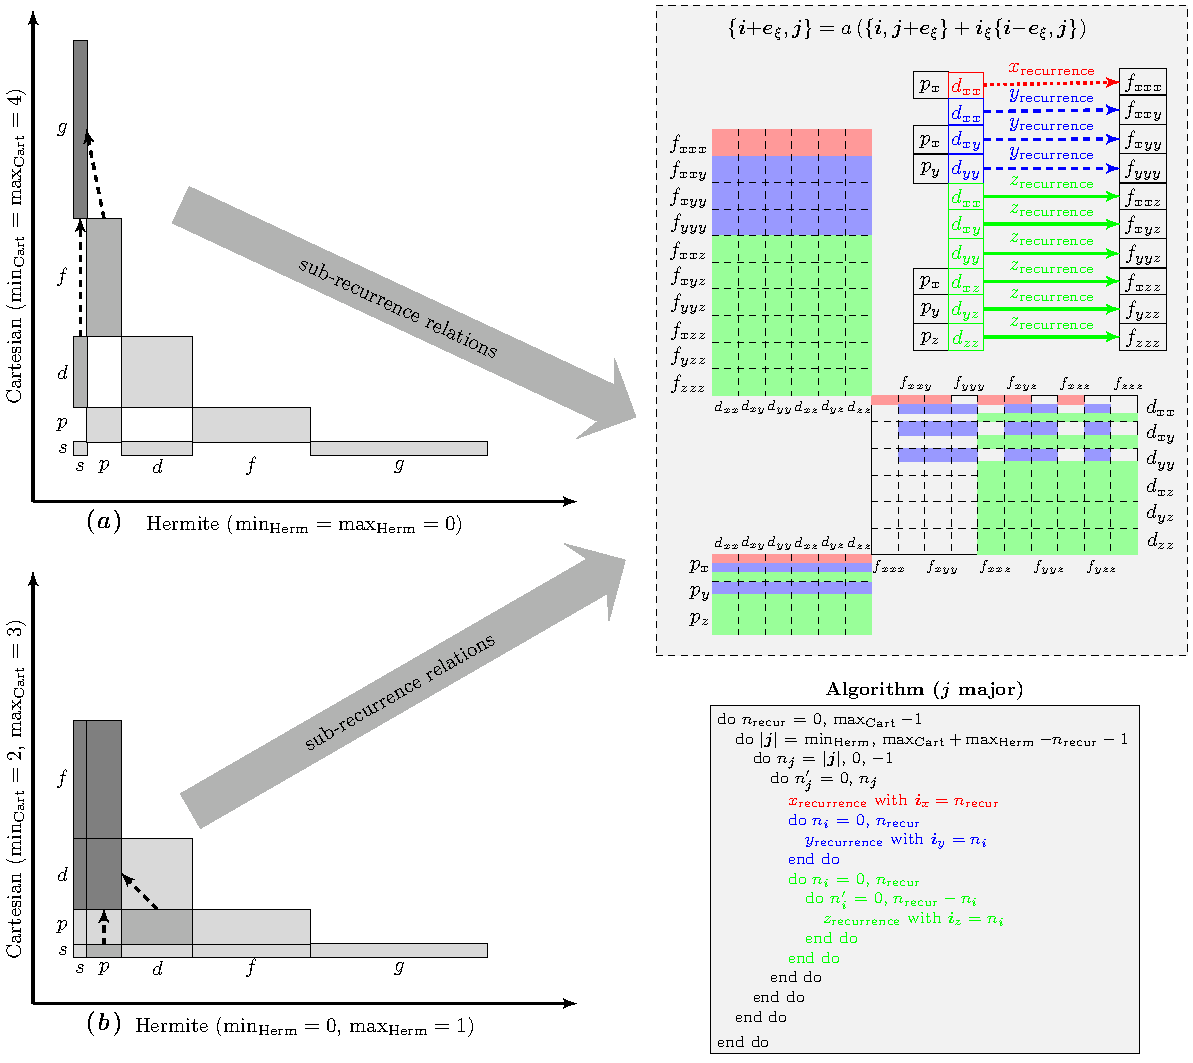
\includegraphics[width=6.8in]{hgto_to_cgto.pdf}
  \caption{Procedure of transformation between Cartesian and Hermite Gaussians.}
  \label{fig:hgto-to-cgto}
\end{figure}

Furthermore, a more detailed version of $\{\boldsymbol{i},\boldsymbol{j}\mathrm{+}\boldsymbol{e}_{\xi}\}%
\Rightarrow\{\boldsymbol{i}\mathrm{+}\boldsymbol{e}_{\xi},\boldsymbol{j}\}$ is given in Fig.~\ref{fig:recurr-dim2-type1}.
\begin{figure}[hbtp]
  \centering
  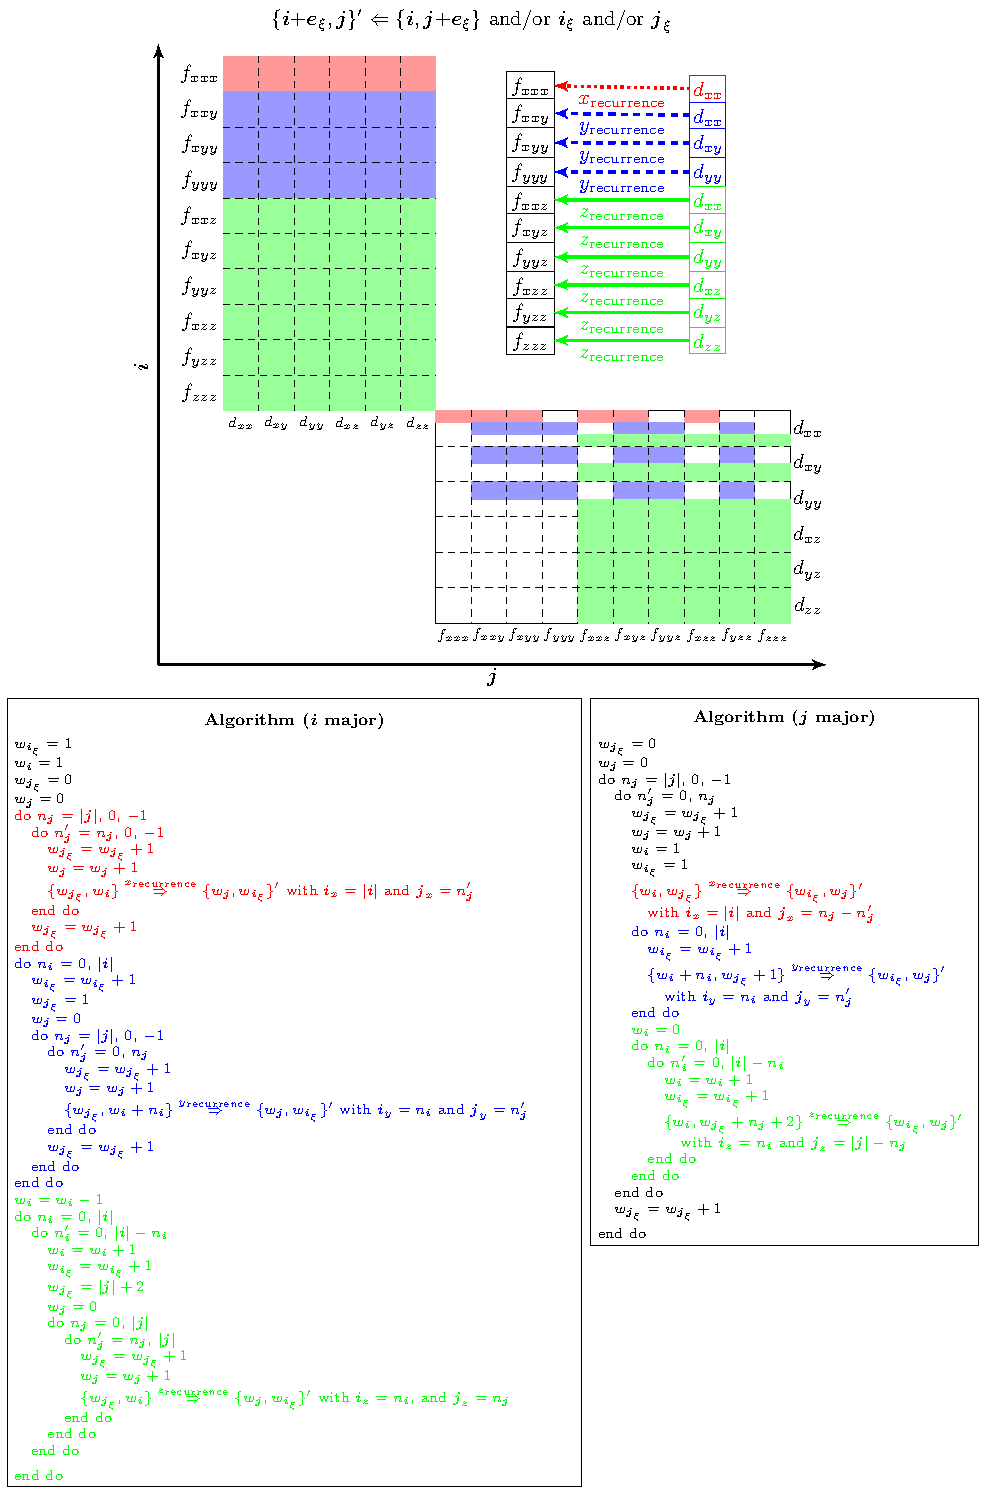
\includegraphics[width=5.2in]{recurr_dim2_type1.pdf}
  \caption{Procedure of $\{\boldsymbol{i},\boldsymbol{j}\mathrm{+}\boldsymbol{e}_{\xi}\}%
\Rightarrow\{\boldsymbol{i}\mathrm{+}\boldsymbol{e}_{\xi},\boldsymbol{j}\}$.}
  \label{fig:recurr-dim2-type1}
\end{figure}

% auxiliary functions
\section{Auxiliary Functions in \textsc{Gen1Int}}
\label{sect:auxfun}

As shown in Section~\ref{sect:operators}, the integrals of some operators needs the knowledge of
special functions. We will therefore focus on the evaluation of auxiliary functions in \textsc{Gen1Int}.
In particular, we will also discuss the limitations of current routines in \textsc{Gen1Int}, which may
point out further development.

% Boys function
\subsection{Boys function}
\label{subsec:boys}

Boys function is defined as
\begin{equation}
  \label{eq:boys-definition}
  F_{n}(T)=\int_0^1\exp[-Tu^2]u^{2n}\mathrm{d}u,
\end{equation}
which is used for nuclear attraction potential, Gaussian charge potential, diamagnetic spin-orbit coupling,
and model core potential (Version 1) ...

\fixme{Describe} subroutines in \verb|aux_boys_vec.F90| ...

% G function
\subsection{Function $G_{n}(T)$}
\label{subsec:gfunc}

The function $G_{n}(T)$ ($n\ge0$, $T\ge0$) is defined as
\begin{equation}
  \label{eq:gfunc-definition}
  G_{n}(T)=\int_0^1\exp[-T(1-u^2)]u^{2n}\mathrm{d}u,
\end{equation}
which is used for inverse square distance potential ...

\fixme{Describe} subroutines in \verb|aux_boys_gfun.F90| ...

% scaled modified spherical Bessel function of the first kind
\subsection{Scaled Modified Spherical Bessel Function of the First Kind}
\label{subsec:bessel}

The scaled modified spherical Bessel function of the first kind is defined as
\begin{equation}
  \mathrm{e}^{-x}M_{n}(x)=\mathrm{e}^{-x}x^{n}\left(\frac{1}{x}\frac{\mathrm{d}}{\mathrm{d}x}\right)^{n}\frac{\sinh x}{x},
\end{equation}
where $M_{n}(x)$ is the so-called modified spherical Bessel function of the first kind.
The scaled modified spherical Bessel function of the first kind is used when calculating
the integrals of effective core potential. Its evaluation has been discussed in
Ref.~\cite{Flores-Moreno:JCC27:1009} ...

\fixme{Describe} subroutines in \verb|aux_msphi_vec.F90| ...

% test suite
\section{Test Suite of \textsc{Gen1Int}}
\label{sect:test-suite}

There are around 30,000 lines source code in \textsc{Gen1Int}, and most of them are designed for
different recurrence relations. Therefore, a ``complete'' and ``thorough'' test suite of all the subroutines
is vital for \textsc{Gen1Int}. The source codes of Fortran 90 test suite are in the directory \verb|test_f90|,
and those of Python test suite are in \verb|tests|. The tests of recurrence relations are usually performed
by comparing the results from \textsc{Gen1Int} and those from recursive functions in Fortran 90 and Python.
Other tests are normally carried out by comparing with the predefined referenced results. Please see the
comments of individual source code for further details.

Fortran 90 test suite will generate an HTML log file called \verb|test_gen1int.html|, please check it carefully
if there is any error (marked in red color). You could also report the errors together with the information of
operating system and compilers to the authors.

We should however emphasize that we release \textsc{Gen1Int} WITHOUT ANY WARRANTY as claimed
in the copyright page. We will nonetheless do our best to make \textsc{Gen1Int} be useful and the functionalities
have been tested to the best of our ability.

\fixme{Adding finite difference tests (order by order to 10?) using primitive and contracted GTOs (moving bra and operator center),
with different situations: (1) bra, ket, operator centers are quite close, (2) bra center is far away from the other
two, (3) ket center is far away from the other two, (4) operator center is far away from the other two,
(5) all of them are far away from each other.}

\subsection{Testing Dashboard of \textsc{Gen1Int}}
\label{sect:CDash}

\begin{enumerate}
  \item Create a file \verb|cmake/Tests.cmake| in which \verb|tools/runtest.sh| returns a 0 if the test passes
    and 1 (or something nonzero) if it fails;
  \item Create \verb|CTestConfig.cmake|;
  \item Set up CDash and CTest in \verb|CMakeLists.txt|;
  \item Try \verb|make test|, \verb|make Experimental| or \verb|make Nightly| (put it into \verb|crontab|);
  \item Check \url{http://repo.ctcc.no/CDash/index.php?project=Gen1Int}.
\end{enumerate}

% Gen1Int subroutines
\chapter{\textsc{Gen1Int} Subroutines}
\label{sect:subroutines}

In this section, we give the list of all public and private \textsc{Gen1Int} subroutines according to
their categories. \fixme{need to add more implemented subroutines ...}

% public subroutines
\section{Public \textsc{Gen1Int} Subroutines}
\label{sect:public-sub}

``\textbf{Public}'' subroutines are those that could be called by users in their own codes.

\begin{enumerate}
  \item Utilities
    \begin{enumerate}
      \item \verb|norm_contr_cgto|, see Table~;
      \item \verb|norm_contr_sgto|, see Table~;
      \item \verb|reorder_sgtos|, see Table~\ref{tab:gen1int-reorder};
      \item \verb|reorder_sgto_ints|, see Table~\ref{tab:gen1int-reorder};
      \item \verb|reorder_cgtos|, see Table~\ref{tab:gen1int-reorder};
      \item \verb|reorder_cgto_ints|, see Table~\ref{tab:gen1int-reorder};
      \item \verb|trace_sgto_ints|, see Table~;
      \item \verb|trace_cgto_ints|, see Table~;
      \item \verb|trace_gto_ints|, see Table~;
    \end{enumerate}
%
  \item Geometric derivatives
  \begin{enumerate}
    \item \verb|geom_total_tree_init|, see Table~\ref{tab:geom-total};
    \item \verb|geom_total_tree_search|, see Table~\ref{tab:geom-total};
  \end{enumerate}
%
  \item Contracted integrals with Cartesian or spherical Gaussians
  \begin{enumerate}
    \item Cartesian multipole moments
    \begin{enumerate}
      \item \verb|contr_cgto_carmom|, see Table~;
      \item \verb|contr_sgto_carmom|, see Table~;
    \end{enumerate}
    \item $\delta$-function
    \begin{enumerate}
      \item \verb|contr_cgto_delta|, see Table~;
      \item \verb|contr_sgto_delta|, see Table~;
    \end{enumerate}
    \item nuclear attraction potential
    \begin{enumerate}
      \item \verb|contr_cgto_nucpot|, see Table~;
      \item \verb|contr_sgto_nucpot|, see Table~;
    \end{enumerate}
    \item inverse square distance potential
    \begin{enumerate}
      \item \verb|contr_cgto_isdpot|, see Table~;
      \item \verb|contr_sgto_isdpot|, see Table~;
    \end{enumerate}
    \item Gaussian charge potential
    \begin{enumerate}
      \item \verb|contr_cgto_gaupot|, see Table~;
      \item \verb|contr_sgto_gaupot|, see Table~;
    \end{enumerate}
    \item diamagnetic spin-orbit coupling
    \begin{enumerate}
      \item \verb|contr_cgto_dso|, see Table~;
      \item \verb|contr_sgto_dso|, see Table~;
    \end{enumerate}
    \item effective core potential
    \begin{enumerate}
      \item \verb|contr_cgto_ecp_local|, see Table~;
      \item \verb|contr_cgto_ecp_non|, see Table~;
      \item \verb|contr_sgto_ecp_local|, see Table~;
      \item \verb|contr_sgto_ecp_non|, see Table~;
    \end{enumerate}
    \item model core potential (Version 1)
    \begin{enumerate}
      \item \verb|contr_cgto_mcp1_pot|, see Table~;
      \item \verb|contr_cgto_mcp1_core|, see Table~;
      \item \verb|contr_sgto_mcp1_pot|, see Table~;
      \item \verb|contr_sgto_mcp1_core|, see Table~;
    \end{enumerate}  
  \end{enumerate}
%
  \item Contracted integrals with rotational London atomic orbitals 
  \begin{enumerate}
    \item Cartesian multipole moments
    \begin{enumerate}
      \item \verb|lcgto_zero_carmom|, see Table~;
      \item \verb|lsgto_zero_carmom|, see Table~;
    \end{enumerate}
    \item $\delta$-function
    \begin{enumerate}
      \item \verb|lcgto_zero_delta|, see Table~;
      \item \verb|lsgto_zero_delta|, see Table~;
    \end{enumerate}
    \item nuclear attraction potential
    \begin{enumerate}
      \item \verb|lcgto_zero_nucpot|, see Table~;
      \item \verb|lsgto_zero_nucpot|, see Table~;
    \end{enumerate}
    \item inverse square distance potential
    \begin{enumerate}
      \item \verb|lcgto_zero_isdpot|, see Table~;
      \item \verb|lsgto_zero_isdpot|, see Table~;
    \end{enumerate}
    \item Gaussian charge potential
    \begin{enumerate}
      \item \verb|lcgto_zero_gaupot|, see Table~;
      \item \verb|lsgto_zero_gaupot|, see Table~;
    \end{enumerate}
    \item diamagnetic spin-orbit coupling
    \begin{enumerate}
      \item \verb|lcgto_zero_dso|, see Table~;
      \item \verb|lsgto_zero_dso|, see Table~;
    \end{enumerate}
    \item effective core potential
    \begin{enumerate}
      \item \verb|lcgto_zero_ecp_local|, see Table~;
      \item \verb|lcgto_zero_ecp_non|, see Table~;
      \item \verb|lsgto_zero_ecp_local|, see Table~;
      \item \verb|lsgto_zero_ecp_non|, see Table~;
    \end{enumerate}
    \item model core potential (Version 1)
    \begin{enumerate}
      \item \verb|lcgto_zero_mcp1_pot|, see Table~;
      \item \verb|lcgto_zero_mcp1_core|, see Table~;
      \item \verb|lsgto_zero_mcp1_pot|, see Table~;
      \item \verb|lsgto_zero_mcp1_core|, see Table~;
    \end{enumerate}  
  \end{enumerate}
\end{enumerate}

% private subroutines
\section{Private \textsc{Gen1Int} Subroutines}
\label{sect:private-sub}

``\textbf{Private}'' subroutines are usually not be called by the users, but used inside \textsc{Gen1Int}.

\begin{enumerate}
  \item Utilities
  \begin{enumerate}
    \item subroutines \verb|xtimer_set| and \verb|xtimer_view| in file \verb|xtimer.F90|, print the CPU
      elapsed time of individual \textsc{Gen1Int} subroutine\footnote{The CPU elapsed time is got from
      the intrinsic function \texttt{cpu}\_\texttt{time}.}, enabled by \verb|-DXTIME| in compiler option;
    \item subroutines \verb|dump_gto_deriv|, \verb|dump_gen_opt|, \verb|dump_ecp|, \verb|dump_mcp1_pot|,
      and \verb|dump_mcp1_core| in file \verb|dump_info.F90| print the information of basis sets,
      operators and derivatives during calculations, enabled by \verb|-DDEBUG| in compiler option;
    \item subroutines \verb|dbinom_coeff| and \verb|pascal_triangle|\footnote{The numbers of Pascal's triangle
      are real type.} in file \verb|binom_coeff.F90| computes the binomial coefficient and Pascal's triangle, respectively;
    \item subroutines \verb|sort_gen_cents| and \verb|sort_atom_cents| in file \verb|sort_cents.F90|
      sort the given centers in descending order, \verb|sort_gen_cents| accepts non-atomc centers (such as dipole origin)
      whose indices are greater than defined variable \verb|MAX_IDX_NON| ($=0$) in \verb|max_idx_non.h|;
    \item \verb|shell_scatter|, see Section~\ref{subsec:geom-part};
    \item \verb|shell_gather|, see Section~\ref{subsec:geom-part};
    \item subroutine \verb|const_contr_ints| in file \verb|const_contr_ints.F90| performs the contractions~(\ref{eq:nonlao-aux-int-cart})
      and (\ref{eq:nonlao-aux-int-herm});
  \end{enumerate}
%
  \item Basis sets transformations
  \begin{enumerate}
    \item \verb|hgto_to_cgto|, see Section~\ref{subsec:hgto-to-cgto};
    \item \verb|hgto_to_cgto_p|, see Section~\ref{subsec:hgto-to-cgto};
    \item \verb|hgto_to_cgto_d|, see Section~\ref{subsec:hgto-to-cgto};
    \item \verb|sub_hgto_to_cgto|, see Section~\ref{subsec:hgto-to-cgto};
    \item \verb|hgto_to_lcgto|, see Section~\ref{subsec:hgto-to-cgto};
  \end{enumerate}
%
  \item Geometric derivatives
  \begin{enumerate}
    \item \verb|geom_total_num_paths|, see Table~\ref{tab:geom-total};
    \item \verb|geom_total_new_path|, see Table~\ref{tab:geom-total};
    \item \verb|geom_part_zero_param|, see Section~\ref{subsec:geom-part};
    \item \verb|geom_part_zero_scatter|, see Section~\ref{subsec:geom-part};
    \item \verb|geom_part_one_param|, see Section~\ref{subsec:geom-part};
    \item \verb|geom_part_one_scatter|, see Section~\ref{subsec:geom-part};
    \item \verb|geom_part_two_param|, see Section~\ref{subsec:geom-part};
  \end{enumerate}
%
  \item Geometric derivatives of dipole origin, \verb|carmom_deriv|, see Section~\ref{subsec:carmom};
%
  \item Cartesian multipole moment integrals
  \begin{enumerate}
    \item \verb|contr_cgto_carmom_recurr|, see Table~;
    \item \verb|prim_hgto_carmom|, see Table~;
    \item \verb|carmom_hrr_ket|, see Section~\ref{subsec:carmom};
    \item \verb|sub_carmom_hrr_ket|, see Section~\ref{subsec:carmom};
    \item \verb|carmom_hbra|, see Section~\ref{subsec:carmom};
    \item \verb|carmom_moment|, see Section~\ref{subsec:carmom};
    \item \verb|carmom_moment_p|, see Section~\ref{subsec:carmom};
    \item \verb|sub_carmom_moment|, see Section~\ref{subsec:carmom};
  \end{enumerate}
%
  \item $\delta$-function
  \begin{enumerate}
    \item \verb|xxxx|, see Table~;
    \item \verb|xxxx|, see Table~;
  \end{enumerate}
%
  \item Nuclear attraction potential
  \begin{enumerate}
    \item \verb|nucpot_geom|, see Section~\ref{subsec:nucpot};
    \item \verb|sub_nucpot_geom_d|, see Section~\ref{subsec:nucpot};
  \end{enumerate}
%
  \item Inverse square distance potential
  \begin{enumerate}
    \item \verb|xxxx|, see Table~;
    \item \verb|xxxx|, see Table~;
  \end{enumerate}
%
  \item Gaussian charge potential
  \begin{enumerate}
    \item \verb|xxxx|, see Table~;
    \item \verb|xxxx|, see Table~;
  \end{enumerate}
%
  \item Diamagnetic spin-orbit coupling
  \begin{enumerate}
    \item \verb|xxxx|, see Table~;
    \item \verb|xxxx|, see Table~;
  \end{enumerate}
%
  \item Effective core potential
  \begin{enumerate}
    \item \verb|xxxx|, see Table~;
    \item \verb|xxxx|, see Table~;
  \end{enumerate}
%
  \item Model core potential (Version 1)
  \begin{enumerate}
    \item \verb|xxxx|, see Table~;
    \item \verb|xxxx|, see Table~;
  \end{enumerate}
%
  \item Quadrature
  \begin{enumerate}
    \item \verb|xxxx|, see Table~;
    \item \verb|xxxx|, see Table~;
  \end{enumerate}
%
  \item Auxiliary functions
  \begin{enumerate}
    \item Boys function
    \begin{enumerate}
      \item \verb|xxxx|, see Table~;
      \item \verb|xxxx|, see Table~;
    \end{enumerate}
    \item Function $G_{n}(T)$
    \begin{enumerate}
      \item \verb|xxxx|, see Table~;
      \item \verb|xxxx|, see Table~;
    \end{enumerate}
    \item Scaled Modified Spherical Bessel Function of the First Kind
    \begin{enumerate}
      \item \verb|xxxx|, see Table~;
      \item \verb|xxxx|, see Table~;
    \end{enumerate}
  \end{enumerate}
\end{enumerate}

% files and directories of Gen1Int
\chapter{Files and Directories of \textsc{Gen1Int}}
\label{chap:gen1int-files}

\fixme{We will list all the files and directories} of \textsc{Gen1Int}, with a brief description ...

% header files
\section{Header Files in \textsc{Gen1Int}}
\label{sect:header-files}

\fixme{We will describe} the header files in directory \verb|src|, some of them may be modified to
satisfy the requirement of users ...

\begin{enumerate}
  \item \verb|xkind.h|: kind type parameter of real numbers
  \item \verb|stdout.h|: IO unit of standard output
  \item \verb|pi.h|: constant $\pi$
  \item \verb|tag_cent.h|: marking the sequence of bra, ket and operator centers
  \item \verb|hgto_to_sgto.h|: parameters related to the transformation between HGTOs and SGTOs
  \item \verb|max_idx_non.h|: maximum index of non-atomic centers
  \item \verb|boys_power.h|: used by power series expansion of Boys function (generated by \verb|tools/GenHeader.py|)
  \item \verb|max_gen_order.h|: maximum order for \textsc{Gen1Int} (generated by \verb|tools/GenHeader.py|)
  \item \verb|tab_boys.h|: pretabulated Boys functions (generated by \verb|tools/GenHeader.py|)
\end{enumerate}

% limitations
\chapter{Limitations of \textsc{Gen1Int}}
\label{chap:limitations}

\fixme{The limitations} of \textsc{Gen1Int} may come from the accuracy of auxiliary functions,
the huge number of derivatives (lots of memory consumed), the accuracy due to large distance
between basis set centers and operator center (will it be a problem?) ...

\textsc{Gen1Int} might not be efficient ...

We describe our future long- and short-term developments in file \verb|TODO| ...

\fixme{When $C$ is far away from $P$, Eq.~(\ref{eq:r-1-aux-ints}) are really some small numbers (unless we have large total exponent), positive and negative, one by one. Therefore, we might have two small number subtraction in Eq.~(\ref{eq:r-1-geo-c}) (remind that Boys function decays quickly, so multiplied by a large $X_{CP}$ might still result in a small number), which as you know may be unstable.}

\fixme{Another thing is related to the evaluation of Boys function, for the time being, Gen1Int provides the Boys function with accuracy, at least, around $10^{-12}$ or $10^{-13}$ (for some arguments it might be even better). For your information, although we have encountered such problem, Gen1Int will stop with error message if the argument and order of Boys function can not be calculated with required accuracy.}

\fixme{Therefore, based on the above two points (small numbers in recurrence relations and the accuracy of Boys functions), Gen1Int might have problem to give accurate enough results when EFG center is far away from the product center.}

\fixme{Instead of first recovering derivatives on EFG center $C$, we could also first recover GTOs on bra and ket center, and get the derivatives on EFG center at last. However, this is more or less the same as what is implemented in Dalton now. And, we can say it is not stable from your tests.}

\fixme{Therefore, to summarize, although Gen1Int might have problem but its current solution is better than EFGINT in Dalton, and we have to trust it ;-)}

\fixme{P.S: Further improvement of Gen1Int could be:}

\fixme{(1) return zero integrals when bra and ket centers are far away;}

\fixme{(2) improve the accuracy of Boys functions, which could be done, and I also have some idea (for instance, increasing the accuracy of pretabulated table of Boys functions, improve the accuracy of modified asymptotic series expansion and upward recurrence relation--which is the key point);}

\fixme{(3) uses more stable recurrence relations or reduce the chance of two small or two big number operations, which I have no idea for the time being.}

% back end
\backmatter

% references
\begin{small}
  \bibliographystyle{unsrt}
%  \bibliographystyle{abbrv}
  \bibliography{refs}
\end{small}

% index
\printindex

\end{document}
